\documentclass[12pt]{niuthesis}
% \documentclass[12pt,singlespacing]{niuthesis}

% some packages are loaded here
\usepackage{lineno}
\usepackage{latexsym}		% to get LASY symbols
\usepackage{graphicx}		% to insert PostScript figures
\usepackage{cancel}
\usepackage{rotating}           % defines sidways table and figure env.
\usepackage{multicol}
% default env and hepunits has issues with degree - workaround 
\usepackage{savesym}
\savesymbol{degree}
\usepackage{hepunits}
\usepackage{amssymb}
\usepackage{amsmath}
\usepackage[hidelinks]{hyperref}
\usepackage[acronym]{glossaries}
\usepackage[style=numeric-comp,sorting=none,block=ragged,firstinits=true]{biblatex}
\renewbibmacro{in:}{}
\bibliography{biblio}
% \addbibressource{biblio}


\usepackage[titletoc]{appendix} % Get appendix on own page
\usepackage{xcolor}
\usepackage{xspace}
\usepackage{microtype}
\usepackage[utf8]{inputenc}
\usepackage{tabularx}
\usepackage{makecell}
\newcolumntype{Y}{>{\centering\arraybackslash}X}

\usepackage{tikz}
\usetikzlibrary{shapes.geometric, arrows}

\font\eightss=cmssq8
\font\eightssi=cmssqi8
\newcommand\quoteAuthor[2]{\begingroup
  \baselineskip 10pt
  \parfillskip 0pt
  \interlinepenalty 10000 % not needed in example
  \leftskip 0pt plus 40pc minus \parindent
  \let\rm=\eightss
  \let\sl=\eightssi
  \everypar{\sl}#1\par
  \nobreak\smallskip
  \noindent\rm--- #2\unskip\par
\endgroup}


% \usepackage{subfig}
\usepackage{subcaption}
\usepackage{multirow} % Table formatting
\usepackage{tablefootnote}
\usepackage{array,booktabs}
\usepackage{dcolumn}

\let\degree\relax

\restoresymbol{DEFAULT}{degree} % make sure this is ok
% \usepackage{hyperref}		% to insert hyperrefs

%%%%%%%%%%%%%%%%%%%%%%%%%%%%%%%%%%%%%%%%%%%%%%%%%%%%%%%%%%%%%%%%
% Some LaTeX macros
\newcommand{\twochoices}[2]{\left\{ \begin{array}{lcc}
        \displaystyle #1 \\ \vspace{-10pt} \\
        \displaystyle #2 \end{array} \right. } %}

\newcommand{\twovec}[2]{\left(\begin{array}{c} #1 \\ #2 \end{array}\right)}

\newcommand{\twomatrix}[4]{\left(\begin{array}{cc} #1 & #2 \\ 
     #3 & #4 \end{array}\right)}

% Uncomment the following line for a List of Symbols
% \newcommand{\listofXXX}{\input{symbols}}

%%%%%%%%%%%%%%%%%%%%%%%%%%%%%%%%%%%%%%%%%%%%%%%%%%%%%%%%%%%%%%%%%%
% Choose the chapter(s) / files you want to work with

%%% use this to compile all chapters
%\def\files{ch1,ch2,refs,app1,app2}

%%% use this to work with only one chapter
%\def\files{chapters/abstract}
%\def\files{chapters/chapter1_theory/theory}
%\def\files{chapters/chapter2_experiment/experiment}
%\includeonly{\files}

%%%%%%%%%%%%%%%%%%%%%%%%%%%%%%%%%%%%%%%%%%%%%%%%%%%%%%%%%%%%%%%%%
\usepackage{variable_defs}
\loadglsentries{glossary}
\makenoidxglossaries
\begin{document}
%\linenumbers

\title{Search for Charged Higgs Bosons in the \taulep Final State with \LUMI of \pp Collision Data at \sqs with the ATLAS Experiment}

\author{Elliot Wesley Parrish}

\major{Physics}
\degree{Dissertation}{Ph.D.}{Doctor of Philosophy}
\degreedate{December}{2022}
\department{Department of Physics}
\director{Dhiman Chakraborty and Jahred Adelman}


\begin{abstract}
  %short

%long

This dissertation uses 139 \ifb of \pp collision data collected at a center of mass energy of \sqs by the ATLAS detector to search for charged Higgs bosons decaying to a tau lepton and a neutrino (\HpLong) in association with a leptonically decaying top quark. No significant excess was found, therefore limits are set at the 95\% confidence level on the charged Higgs production cross section times the branching fraction into the \taunu ranging from XX pb to XX fb. These limits are interpreted in the hMSSM benchmark scenario as an exclusion at 95\% confidence on \tanb as a function of \mHp. In this scenario, for $\tanb=60$, the \Hp mass range up to $\unit{XXXX}{GeV}$ is excluded, with all values of \tanb excluded for $\mHp \leq \unit{XXX}{GeV}$
\end{abstract}

\begin{acknowledgments}
  % TODO: ALL OF IT :)
I would like to start by thanking Dhiman Chakraborty for the incredibly opportunity to be your student. Thank you for fighting for me from day one; I would not be here without your efforts. I would like to extend my gratitude to Jahred Adelman for taking me on as a student and ensuring I finish this program. I would also like to thank the rest of my committee for their mentorship. 

Thank you to the incredibly ATLAS and CERN communities, it was a pleasure to work with such dedicated people. Thank you to the Tile community for the unique opportunity to work on all aspects of the machine with experts from across the globe. To name a few, Oleg Solovyanov, Sanya Solodkov, Irakli Minashvili, Siarhei Harkusha, and all of the Charge Injection System experts. Thank you to the charged Higgs analysis group, it has been a truly incredible experience working with you. I'd like to especially thank Pawel Klimek for your guidance throughout this program. Thank you to Michalea Mlynarikova for your support as a friend and mentor over countless cups of coffee. Thank you to the University of Oregon ATLAS group for the many years of guidance. Thank you to the other NIU graduate students and the ATLAS group.

Thank you to all of the friends I have made along this journey. John Myers, Ian Snyder, and Jason Barkeloo for welcoming me with open arms all those years ago as an undergraduate who had no idea where he was going. Thank you Tyler Burch for helping guide me through the journey at NIU. Thank you to Jimmy Friedricks, Samantha Freidricks, Hayden Harris, and Kylie Harris for reminding me to enjoy life. To the numerous friends I made while living at CERN, thank you for the memories, I will always look back fondly on our time together. Thank you to Christopher Heath Parent for your unconditional support and brotherhood.

Lastly, I would like to thank my family for their unwavering support. Thank you Amanda Steinhebel for the encouragement, patience, and support to see this to the end.
\end{acknowledgments}

\begin{dedication}
  For Robert Burch and Jim Richardson, for the example you set in work and in love,\\
    
and for Carla Thomure, for showing me how to be truly joyful.

\end{dedication}

% comment this to suppress prologue
\MakeThesisPrologue % includes table of contents
%\tableofcontents{}

\chapter{Introduction}\label{chap:Intro}
	Science has long sought to provide an explanation to the most fundamental questions. The field of particle physics tries to answer  the question of ``What are we made of?'' The \gls{SM} of particle physics is an attempt at combining all of the fundamental forces and particles into one mathematically based theory. The \gls{SM} has been rigorously tested and for the most part, holds up except for a few key issues. To name a few of these issues: the absence of gravity in the theory, no candidate for dark matter, neutrino masses, and the matter-antimatter asymmetry of the universe.

	There are many \gls{BSM} theories that address these issues and more. A common theme of these models is an extended Higgs sector, meaning more Higgs boson-like particles. This dissertation focuses on a search for an additional Higgs boson that carries electromagnetic charge, \Hpm. The search is performed on data collected with the \acrshort{ATLAS} detector on the \gls{LHC} at \gls{CERN} in Geneva, Switzerland. 

	A theoretical motivation is given in Chapter \ref{chap:Theory} followed by a detailed explanation of the \gls{LHC} and the \gls{ATLAS} detector in Chapter \ref{chap:experiment}. Simulation of particle collisions and the reconstruction of both simulated and actual data is detailed in Chapters \ref{chap:sim} and \ref{chap:reco} respectively. Chapter \ref{chap:hpana} provides a thorough description of the search for the \Hpm in the \taunu final state. Lastly future works are discussed in Chapter \ref{chap:conclusions}.

	A considerable amount of the author's time in the Ph.D. program was dedicated towards the search described in this dissertation and acting as the Data Quality Co-Coordinator for the hadronic calorimeter within the \gls{ATLAS} Collaboration. In addition, the author assisted on various projects within the hadronic calorimeter group including two test beams and maintenance of the calorimeter within the larger ATLAS detector.
\chapter{Theory}\label{chap:Theory}
    In this chapter, the theoretical motivation of a search for \HpmLong is described. A review of the \acrfull{SM} of particle physics is laid out, followed by a brief overview of \gls{SUSY} focusing on the \acrfull{MSSM}. Finally, the Type II \acrfull{2HDM} relation to the \Hpm production cross section and subsequent branching ratio into \gls{SM} particles is described as motivation for the choice of studying \HpmLong.

\section{The Standard Model}\label{sec:SM}
	The \gls{SM} of particle physics is a \gls{QFT} that describes all known matter and forces\footnote{Notably, the SM does not describe gravity.}. The \gls{SM} describes forces as exchanges of particles called bosons and is described in detail in Section \ref{ssec:Interactions}. These interactions occur between fundamental particles called fermions that comprise the known matter of the universe. Figure \ref{fig:atom-to-quarks} shows how fermions called quarks are the building blocks of nucleons, and thus atoms.

	\begin{figure}[!ht]
		\centering
		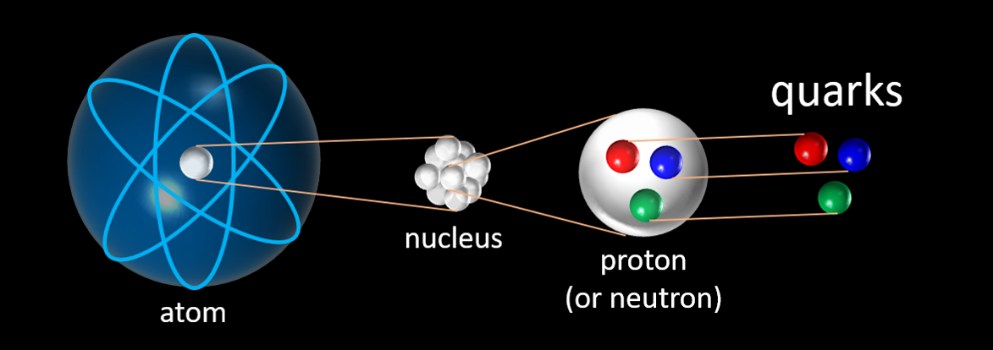
\includegraphics[width=.75\textwidth,keepaspectratio=true]{chapters/chapter2_theory/images/Atom_to_Quark_Cartoon.png}
		\caption{Quarks are fundamental particles that combine to create hadrons (protons, neutrons, $\pi^{0,\pm}$, etc.) \cite{atom-to-quark}.}
		\label{fig:atom-to-quarks}
	\end{figure}

	\subsection{Particles}\label{ssec:Particles}
		The particles that make up the \gls{SM} are defined by their properties, or quantum numbers. These quantum numbers are used to categorize particles into various types. Intrinsic angular momentum charge, or spin, is the first quantum number that separates particles into fermions or bosons. Fermions are those that carry half-integer spin, and thus obey Fermi-Dirac statistics, while bosons carry full integer spin values and obey Bose-Einstein statistics.
		
		\subsubsection{Fermions}\label{sssec:Fermions}
			The matter encountered in everyday life is comprised of fermions. Fermions are subdivided into two groups, quarks and leptons. The quarks participate in the strong interaction via their color charge. Quarks cannot exist as an isolated particle and thus combine into hadrons in a process called hadronization; the bound states they form are colorless. The proton and neutron are examples of hadrons. Hadrons, quarks, and their interaction with the strong force are detailed in Section \ref{sssec:QCD}. Leptons carry no color charge and therefore do not participate in strong force interactions. The fermions in the \gls{SM} all participate in the electroweak interaction. However, the electromagnetic interaction is limited to those fermions that carry an electromagnetic charge. Section \ref{sssec:Electroweak} describes the electroweak interaction in detail.

			Fermions can then be further divided into three generations, each lepton has an electrically neutral weak force partner in the form of a neutrino. Table \ref{tab:fermions} lists all the \gls{SM} fermions and their properties. Every particle has a partner with identical properties except for an opposite \gls{EM} charge. These partners are called antimatter and are denoted with a bar above the particle symbol $(u, \bar{u})$.

			\begin{table}[!thp]
				% \centering
				\caption{Standard Model fermions and their properties \cite{pdg}.}
				\resizebox{\textwidth}{!}{\begin{tabular}{c | c | c | c | c | c | c | c |}
				\cline{2-8}

																& \begin{tabular}[c]{@{}c@{}}$1^{st}$ \\ Generation \end{tabular} & \begin{tabular}[c]{@{}c@{}} $2^{nd}$ \\ Generation \end{tabular} 	& \begin{tabular}[c]{@{}c@{}} $3^{rd}$ \\ Generation \end{tabular}	& Spin 			& \begin{tabular}[c]{@{}c@{}}EM \\Charge \end{tabular}		& Color 		& Mass \\[1ex] \hline
				\multicolumn{1}{|c|}{\multirow{3}{*}{Quarks}}   & Up (u)						& Charm (c)						& Top (t)						& $\frac{1}{2}$ & $+\frac{2}{3}$	& \scalecheck  	& \begin{tabular}[c]{@{}c@{}} $m_u = 2.16^{+0.49}_{-0.26}$ MeV \\[1ex] $m_c = 1.27 \pm 0.02$ GeV \\[1ex] $m_t = 172.76 \pm 0.30$ GeV \end{tabular}		\\[1ex] \cline{2-8}
				\multicolumn{1}{|l|}{}                         	& Down (d)						& Strange (s)					& Bottom (b) 					& $\frac{1}{2}$ & $-\frac{1}{3}$	& \scalecheck	& \begin{tabular}[c]{@{}c@{}} $m_d = 4.67^{+0.48}_{-0.17}$ MeV \\[1ex] $m_s = 93^{11}_{-5}$ MeV \\[1ex] $m_b = 4.18^{0.03}_{-0.02}$ GeV \end{tabular}				\\[1ex]	\hline
				\multicolumn{1}{|c|}{\multirow{3}{*}{Leptons}}  & Electron ($e^{-}$)			& Muon ($\mu^{-}$)				& Tau ($\tau^{-}$)				& $\frac{1}{2}$ & $-1$ 				& X 			& \begin{tabular}[c]{@{}c@{}} $m_{e^{-}} = 0.51$ MeV \\[1ex] $m_{\mu^{-}} = 105.65$ MeV \\[1ex] $m_{\tau^{-}} = 1776.86 \pm 0.12$ MeV \end{tabular}		\\[1ex] \cline{2-8}
				\multicolumn{1}{|c|}{}  						& \begin{tabular}[c]{@{}c@{}}Electron \\ Neutrino\end{tabular} ($\nu_{e}$)	& \begin{tabular}[c]{@{}c@{}}Muon \\ Neutrino\end{tabular} ($\nu_{\mu}$)	& \begin{tabular}[c]{@{}c@{}}Tau \\ Neutrino\end{tabular} ($\nu_{\tau}$) & $\frac{1}{2}$ & $0$ 				& X 			& \begin{tabular}[c]{@{}c@{}} $m_{\nu_{e}} < 1.1$ eV \\[1ex] $m_{\nu_{\mu}} < 0.19 $ MeV  \\[1ex] $m_{\nu_{\tau}} < 18.2 $ MeV \end{tabular}		\\[1ex] \hline			
				\end{tabular}}
				\label{tab:fermions}
			\end{table}


		\subsubsection{Bosons}\label{sssec:Bosons}
			Bosons are colloquially referred to as force-carriers in that the fundamental forces act via exchanging gauge bosons. This means that each force has associated boson(s) which is described by a field theory. The electroweak \gls{QFT} is more complicated, and is described in detail in section \ref{sssec:Electroweak}. Table \ref{tab:bosons} lists the \gls{SM} bosons\footnote{Excluding the Higgs boson.}, their associated field theory and properties.

			\begin{table}[!thp]
			\centering
			\caption{Standard Model bosons and their properties \cite{pdg}.}
			\resizebox{\textwidth}{!}{\begin{tabular}{| c | c | c | c | c | c |}  
			\hline
			\multicolumn{1}{|c|}{Field Theory}							& Boson 				& Spin 	& \begin{tabular}[c]{@{}c@{}} EM \\ Charge \end{tabular} 	& Color 		& Mass 	\\[1ex] \hline 
			\multicolumn{1}{|c|}{\acrfull{QCD}}			& Gluon (g)				& 1 	& 0 														& \scalecheck 	& 0		\\[1ex] \hline
 			% \multicolumn{1}{|c|}{\acrfull{QED}} 		& Photon ($\gamma$) 	& 1 	& 0 													 	& X 			& $< 1 \, \mathrm{x} \, 10^{-18}$ eV  	\\[1ex] \hline
 			\multicolumn{1}{|c|}{\acrfull{QED}} 		& Photon ($\gamma$) 	& 1 	& 0 													 	& X 			& 0  	\\[1ex] \hline
			\multicolumn{1}{|c|}{\multirow{2}{*}{Electroweak Theory}} 	& $W^{\pm}$ 			& 1 	& $\pm 1$													& X 			& $80.379 \pm 0.012$ GeV	\\[1ex] \cline{2-6}
			\multicolumn{1}{|c|}{} 										& $Z^{0}$				& 1 	& 0 													 	& X 			& $91.1876 \pm 0.0021$ GeV  	\\[1ex] \hline
			\end{tabular}}
			\label{tab:bosons}
			\end{table}

	\subsection{Interactions}\label{ssec:Interactions}
		 The \gls{SM} is based upon conservation laws. These conversation laws are what dictate the allowed interactions of matter. Lepton generation number\footnote{Ignoring neutrino oscillations.}, electric charge, color charge, 4-momentum ($p=(E,\vec{p})$), and angular momentum are all conserved in the \gls{SM}. In strong interactions baryon number\footnote{Here, $n_{q}$ and $n_{\bar{q}}$ are the number of quarks and antiquarks that comprise the baryon.} $(B = \frac{1}{3}(n_{q} - n_{\bar{q}}) )$ is also conserved.
		% The \gls{SM} is built upon a gauge group of type $SU(3)_C \times SU(2)_L \times U(1)_Y$. The $SU(3)_C$ term dictates the strong interaction while the $SU(2)_L \times U(1)_Y$ term describes the electroweak interaction.
		 % At its core, the \gls{SM} relies upon symmetries; from these symmetries, conservation laws follow. It is these laws of conservation that dictate the allowed interactions of matter. The symmetry between charge conjugation and mirror reflection \gls{CP} can be broken in certain circumstances, but holds in strong and electromagnetic interactions. The breaking of \gls{CP} symmetry occurs in the weak interaction and implies an asymmetry between matter and antimatter. Since this symmetry holds for strong and electromagnetic interactions, baryon number\footnote{Here, $n_{q}$ and $n_{\bar{q}}$ are the number of quarks and antiquarks that comprise the baryon.} $(B = \frac{1}{3}(n_{q} - n_{\bar{q}}) )$ and lepton number are conserved in \gls{SM} interactions. Lepton generation number\footnote{Ignoring neutrino oscillations}, electric charge, color charge, 4-momentum ($p=(E,\vec{p})$), and angular momentum are all conserved in the \gls{SM}.
		 % The first, being a symmetry under charge conjugation, mirror reflection, and time reversal is known as \gls{CPT} symmetry.

		\subsubsection{Quantum Electrodynamics}\label{sssec:QED}
			The electromagnetic force is governed by the \gls{QFT} known as \acrfull{QED}. This force is mediated by the photon, $\gamma$, a massless boson with \gls{EM} charge 0. The \gls{EM} force only interacts with electrically charged particles, including all quarks and the $e$, $\mu$, and $\tau$ leptons.

		\subsubsection{Electroweak Interaction}\label{sssec:Electroweak}
			The weak force is most often seen in nuclear decays and is mediated by the $W^{\pm}$ and $Z^0$ bosons. Due to the relatively large mass of these bosons, the weak force has a very limited range. The weak force interacts via the quantum number called weak isospin ($T$). The $W^{\pm}$ affects the third component of weak isospin ($T_3$), thus only coupling to so called left-handed fermions. In this way, $T_{3}$ defines the ``handedness'', or chirality of a particle. At energies $> 100 $ GeV the electromagnetic and weak forces combine into the electroweak force. Isospin and another quantum number hypercharge combine to give \gls{EM} charge. $Q_{EM} = T_3 + \frac{1}{2} Y_W$. Table \ref{tab:weak} contains the allowed values for weak isospin and hypercharge ($Y_W$). 

			\begin{table}[!thp]
					\centering
					\caption{Standard Model fermions and their Electroweak properties \cite{pdg}.}
					\resizebox{\textwidth}{!}{\begin{tabular}{| c | c | c | c | c | c | c | c | c | c | c | c |}
					\hline

																	& \begin{tabular}[c]{@{}c@{}}$1^{st}$ \\ Generation \end{tabular} & \begin{tabular}[c]{@{}c@{}} $2^{nd}$ \\ Generation \end{tabular} 	& \begin{tabular}[c]{@{}c@{}} $3^{rd}$ \\ Generation \end{tabular}		& \begin{tabular}[c]{@{}c@{}}EM \\ Charge \end{tabular} & \multicolumn{2}{|c|}{$Y_{W}$} & \multicolumn{2}{|c|}{T} 	& \multicolumn{2}{|c|}{$T_{3}$} \\ \hline
					& & & & &  LH 				& RH 					& LH 			& RH 				& LH 	& RH \\ \cline{6-11}
					\multicolumn{1}{|c|}{\multirow{3}{*}{Quarks}}   & Up (u)						& Charm (c)						& Top (t)						&  $+\frac{2}{3}$ & $+\frac{1}{3}$	& $+\frac{4}{3}$		& $\frac{1}{2}$	& 0					& $\pm \frac{1}{2}$	 	& 0	 \\[1ex] \cline{2-11}
					\multicolumn{1}{|l|}{}                         	& Down (d)						& Strange (s)					& Bottom (b) 					&  $-\frac{1}{3}$ & $+\frac{1}{3}$	& $-\frac{2}{3}$		& $\frac{1}{2}$	& 0					& $\pm \frac{1}{2}$	 	& 0	 \\[1ex] \hline
					\multicolumn{1}{|c|}{\multirow{3}{*}{Leptons}}  & Electron ($e^{-}$)			& Muon ($\mu^{-}$)				& Tau ($\tau^{-}$)				&  $-1$ & $-1$				& $0$					& $\frac{1}{2}$	& 0					& $\pm \frac{1}{2}$	 	& 0	 \\[1ex] \cline{2-11}
					\multicolumn{1}{|c|}{}  						& \begin{tabular}[c]{@{}c@{}}Electron \\ Neutrino\end{tabular} ($\nu_{e}$)	& \begin{tabular}[c]{@{}c@{}}Muon \\ Neutrino\end{tabular} ($\nu_{\mu}$)	& \begin{tabular}[c]{@{}c@{}}Tau \\ Neutrino\end{tabular} ($\nu_{\tau}$) & $0$ & $-1$				& $-2$					& $\frac{1}{2}$	& 0					& $\pm \frac{1}{2}$	 	& 0	 \\ \hline			
					\end{tabular}}
					\label{tab:weak}
				\end{table}

			The $W^\pm$ bosons have a $T_3$ component of weak isospin and act as raising or lowering operators on the $T_3$ component of left handed fermions. The $Z$ boson does not have a $T_3$ component, and thus does not act on weak isospin of fermions. The Z boson instead transfers momentum, energy, and spin on all fermions irregardless of their chirality. 

			% \begin{table}[!thp]
			% 	\centering
			% 	\caption{Standard Model particles and their electroweak quantum numbers \cite{pdg}}
			% 	\begin{tabular}{| c | c | c | c | c | c | c |}  
			% 	\hline
			% 	Particle 	& \multicolumn{2}{|c|}{$Y_{W}$} & \multicolumn{2}{|c|}{T} 	& \multicolumn{2}{|c|}{$T_{3}$} \\ \hline
			% 				& LH 				& RH 					& LH 			& RH 				& LH 	& RH \\ \hline
			% 	u 			& $+\frac{1}{3}$	& $+\frac{4}{3}$		& $\frac{1}{2}$	& 0					& $\pm \frac{1}{2}$	 	& 0	 \\[1ex] \hline
			% 	d 			& $+\frac{1}{3}$	& $-\frac{2}{3}$		& $\frac{1}{2}$	& 0					& $\pm \frac{1}{2}$	 	& 0	 \\[1ex] \hline
			% 	c 			& $+\frac{1}{3}$	& $+\frac{4}{3}$		& $\frac{1}{2}$	& 0					& $\pm \frac{1}{2}$	 	& 0	 \\[1ex] \hline
			% 	s 			& $+\frac{1}{3}$	& $-\frac{2}{3}$		& $\frac{1}{2}$	& 0					& $\pm \frac{1}{2}$	 	& 0	 \\[1ex] \hline
			% 	t 			& $+\frac{1}{3}$	& $+\frac{4}{3}$		& $\frac{1}{2}$	& 0					& $\pm \frac{1}{2}$	 	& 0	 \\[1ex] \hline
			% 	b 			& $+\frac{1}{3}$	& $-\frac{2}{3}$		& $\frac{1}{2}$	& 0					& $\pm \frac{1}{2}$	 	& 0	 \\[1ex] \hline
			% 	e 			& $-1$				& $0$					& $\frac{1}{2}$	& 0					& $\pm \frac{1}{2}$	 	& 0	 \\[1ex] \hline
			% 	$\nu_e$ 	& $-1$				& $-2$					& $\frac{1}{2}$	& 0					& $\pm \frac{1}{2}$	 	& 0	 \\[1ex] \hline
			% 	$\mu$ 		& $-1$				& $0$					& $\frac{1}{2}$	& 0					& $\pm \frac{1}{2}$	 	& 0	 \\[1ex] \hline
			% 	$\nu_\mu$ 	& $-1$				& $-2$					& $\frac{1}{2}$	& 0					& $\pm \frac{1}{2}$	 	& 0	 \\[1ex] \hline
			% 	$\tau$ 		& $-1$				& $0$					& $\frac{1}{2}$	& 0					& $\pm \frac{1}{2}$	 	& 0	 \\[1ex] \hline
			% 	$\nu_\tau$ 	& $-1$				& $-2$					& $\frac{1}{2}$	& 0					& $\pm \frac{1}{2}$	 	& 0	 \\[1ex] \hline
			% 	$\gamma$ 	& \multicolumn{2}{|c|}{$0$}					& $\frac{1}{2}$	& 0					& $\pm \frac{1}{2}$	 	& 0	 \\[1ex] \hline
			% 	$g$ 		& \multicolumn{2}{|c|}{X}					& $\frac{1}{2}$	& 0					& $\pm \frac{1}{2}$	 	& 0	 \\[1ex] \hline
			% 	$W$ 		& \multicolumn{2}{|c|}{$0$}					& $\frac{1}{2}$	& 0					& $\pm \frac{1}{2}$	 	& 0	 \\[1ex] \hline
			% 	$Z$ 		& \multicolumn{2}{|c|}{$0$}					& $\frac{1}{2}$	& 0					& $\pm \frac{1}{2}$	 	& 0	 \\[1ex] \hline
			% 	$H$ 		& \multicolumn{2}{|c|}{$+1$}				& $\frac{1}{2}$	& 0					& $\pm \frac{1}{2}$	 	& 0	 \\[1ex] \hline
			% 	\end{tabular}
			% 	\label{tab:weak}
			% 	\end{table}

		\subsubsection{Quantum Chromodynamics}\label{sssec:QCD}
		
			\acrfull{QCD} is the \gls{QFT} that describes the strong force which holds together atomic nuclei and other objects called hadrons. The strong force interacts via the color charge\footnote{This color does is not the visual color we are used to; merely a convenient analogous naming scheme.} which can have values of either red, green, or blue. Particles that have a color charge cannot exist on their own, they must form colorless bound states called hadrons. Since the strong force grows with distance, if a quark is ejected out from a hadron, the stored energy is such that new particles with color charge will be spontaneously created from the vacuum, binding with the free quark in a process called hadronization. In a particle detector, the hadronization process cascades and creates showers of hadrons that are reconstructed as so called jets.

	\subsection{The Higgs Mechanism}\label{ssec:Higgs}

		The Higgs field is the mass generator of the \gls{SM} and was first theorized by Peter Higgs \cite{Higgs-paper}, François Englert, and Robert Brout \cite{Englert-Brout} in 1964.  The \gls{SM} itself has four massless bosons, $B$ and $\vec{W}$ $(W_{1,2,3})$, that do not correspond to the observed bosons. Instead, the Higgs mechanism couples to them via a complex scalar doublet ($\phi$): 
		\begin{equation}\label{eqn:scal doub} \phi = \binom{\phi^+}{\phi^0}\end{equation}
		The scalar potential that gives rise to this phenomena can be written as 
		\begin{equation}\label{eqn:higgs potential} V(\phi) = \mu^2 |\phi^{\dagger}\phi| + \lambda (|\phi^{\dagger}\phi|)^2\end{equation}
		When $\mu^2>0$ and $\lambda>0$ the minimum of the potential $V(\phi)$ is 0. 
		\begin{figure}[!ht] \centering 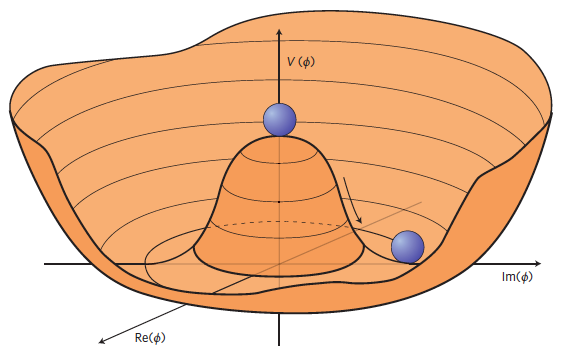
\includegraphics[width=.7\textwidth,keepaspectratio=true]{chapters/chapter2_theory/images/higgspotential.png} \caption{The Higgs potential defined in Equation \ref{eqn:higgs potential} with $\mu^2<0$ \cite{Higgs-phys}.} \label{fig:higgs-potential}\end{figure}
		However, when $\mu^2<0$, the scalar potential $V(\phi)$ takes the shape shown in figure \ref{fig:higgs-potential}.
		It follows that the \gls{VEV} of $\phi$ is then 
		\begin{equation}\label{eqn:higgs vev} \langle \phi \rangle = \sqrt{\frac{-\mu^2}{2\lambda}} = \frac{\nu}{\sqrt{2}}	\end{equation}
		where $\nu = \sqrt{\frac{-\mu^2}{\lambda}}$.
		From here, convention states to choose an arbitrary direction of the fluctuation as 
		\begin{equation}\label{eqn:phi zero} \phi^0 = \frac{1}{\sqrt{2}} \binom{0}{\nu} \end{equation}
		By choosing these values three of the bosons are absorbed in giving mass to the $W^{\pm}$ and $Z^0$ bosons leaving the final as the real scalar field $h(x)$
		\begin{equation}\label{eqn:phi-h} \phi(x) = \phi^0 + h(x) \end{equation}
		Substituting the definition of $\phi^0$ yields
		\begin{equation}\label{eqn:phi-h-vec} \phi = \frac{1}{\sqrt{2}} \binom{0}{\nu+h(x)} \end{equation}
		which couples to the \gls{SM} bosons via
		\begin{equation}\label{eqn:coupling} (\frac{1}{2} g \vec{\sigma} \cdot \vec{W} + \frac{1}{2} g^\prime B ) \phi^0  \end{equation} where $\vec{\sigma}$ are the Pauli matrices, $g$ is the weak coupling constant, and $g^{\prime}$ is the hypercharge coupling constant. From this coupling, there are four eigenstates which correspond to the observed bosons
		\begin{equation}\label{eqn:mass-eigenstates} \begin{split}
		W^\pm = \frac{1}{\sqrt{2}} ( W^1_\mu \mp i W^2_\mu ) \\
		Z^\mu = \frac{ - g\prime B_\mu + g W^3_\mu }{ \sqrt{g^2+g\prime^2} } \\
		A^\mu = \frac{ g B_\mu + g\prime W^3_\mu }{ \sqrt{g^2+g\prime^2} }
		\end{split}
		\end{equation}
		These eigenstates have corresponding mass values of 
		\begin{equation}\label{eqn:mass-eigenstates-masses} \begin{split}
		M^2_W = \frac{1}{4}g^2\nu^2 \\
		M^2_Z = \frac{1}{4}(g^2+g\prime^2)\nu \\
		M^2_A = 0
		\end{split}
		\end{equation}
		The eigenstate labeled here as $A$ is the photon. The Higgs boson was discovered in 2012 by the \gls{ATLAS} and \gls{CMS} collaborations at \gls{CERN} with a mass of $125$ GeV \cites{higgs-discovery-atlas}{CMS-Higgs-Discovery}. The \gls{ATLAS} result in the $H \to \gamma \gamma$ can be seen in Figure \ref{fig:higgs-discovery}. The scalar boson that was found appears to be the \gls{SM} Higgs Boson with the properties shown in Table \ref{tab:higgs-properties}.

		\begin{table}[!thp]
			\centering
			\caption{The Higgs boson's properties \cite{pdg}.}
			\resizebox{.8\textwidth}{!}{\begin{tabular}{| c | c | c | c | c | c | c | c |}  
			\hline
			\multicolumn{1}{|c|}{Field Theory}				& Boson 				& Spin 	& \begin{tabular}[c]{@{}c@{}} EM \\ Charge \end{tabular} 	& Color 		& Mass 	 					& $Y_{W}$ 			& $T_{3}$ 	\\ \hline 
			\multicolumn{1}{|c|}{Higgs Mechanism}			& Higgs (H)				& 0 	& 0 														& X 			& $125.25 \pm 0.17$ GeV		& $\pm\frac{1}{2}$	& $\mp 1$	\\[1.5ex] \hline
			\end{tabular}}
			\label{tab:higgs-properties}
		\end{table}

		% \begin{figure}[!ht]
		% \centering
		% 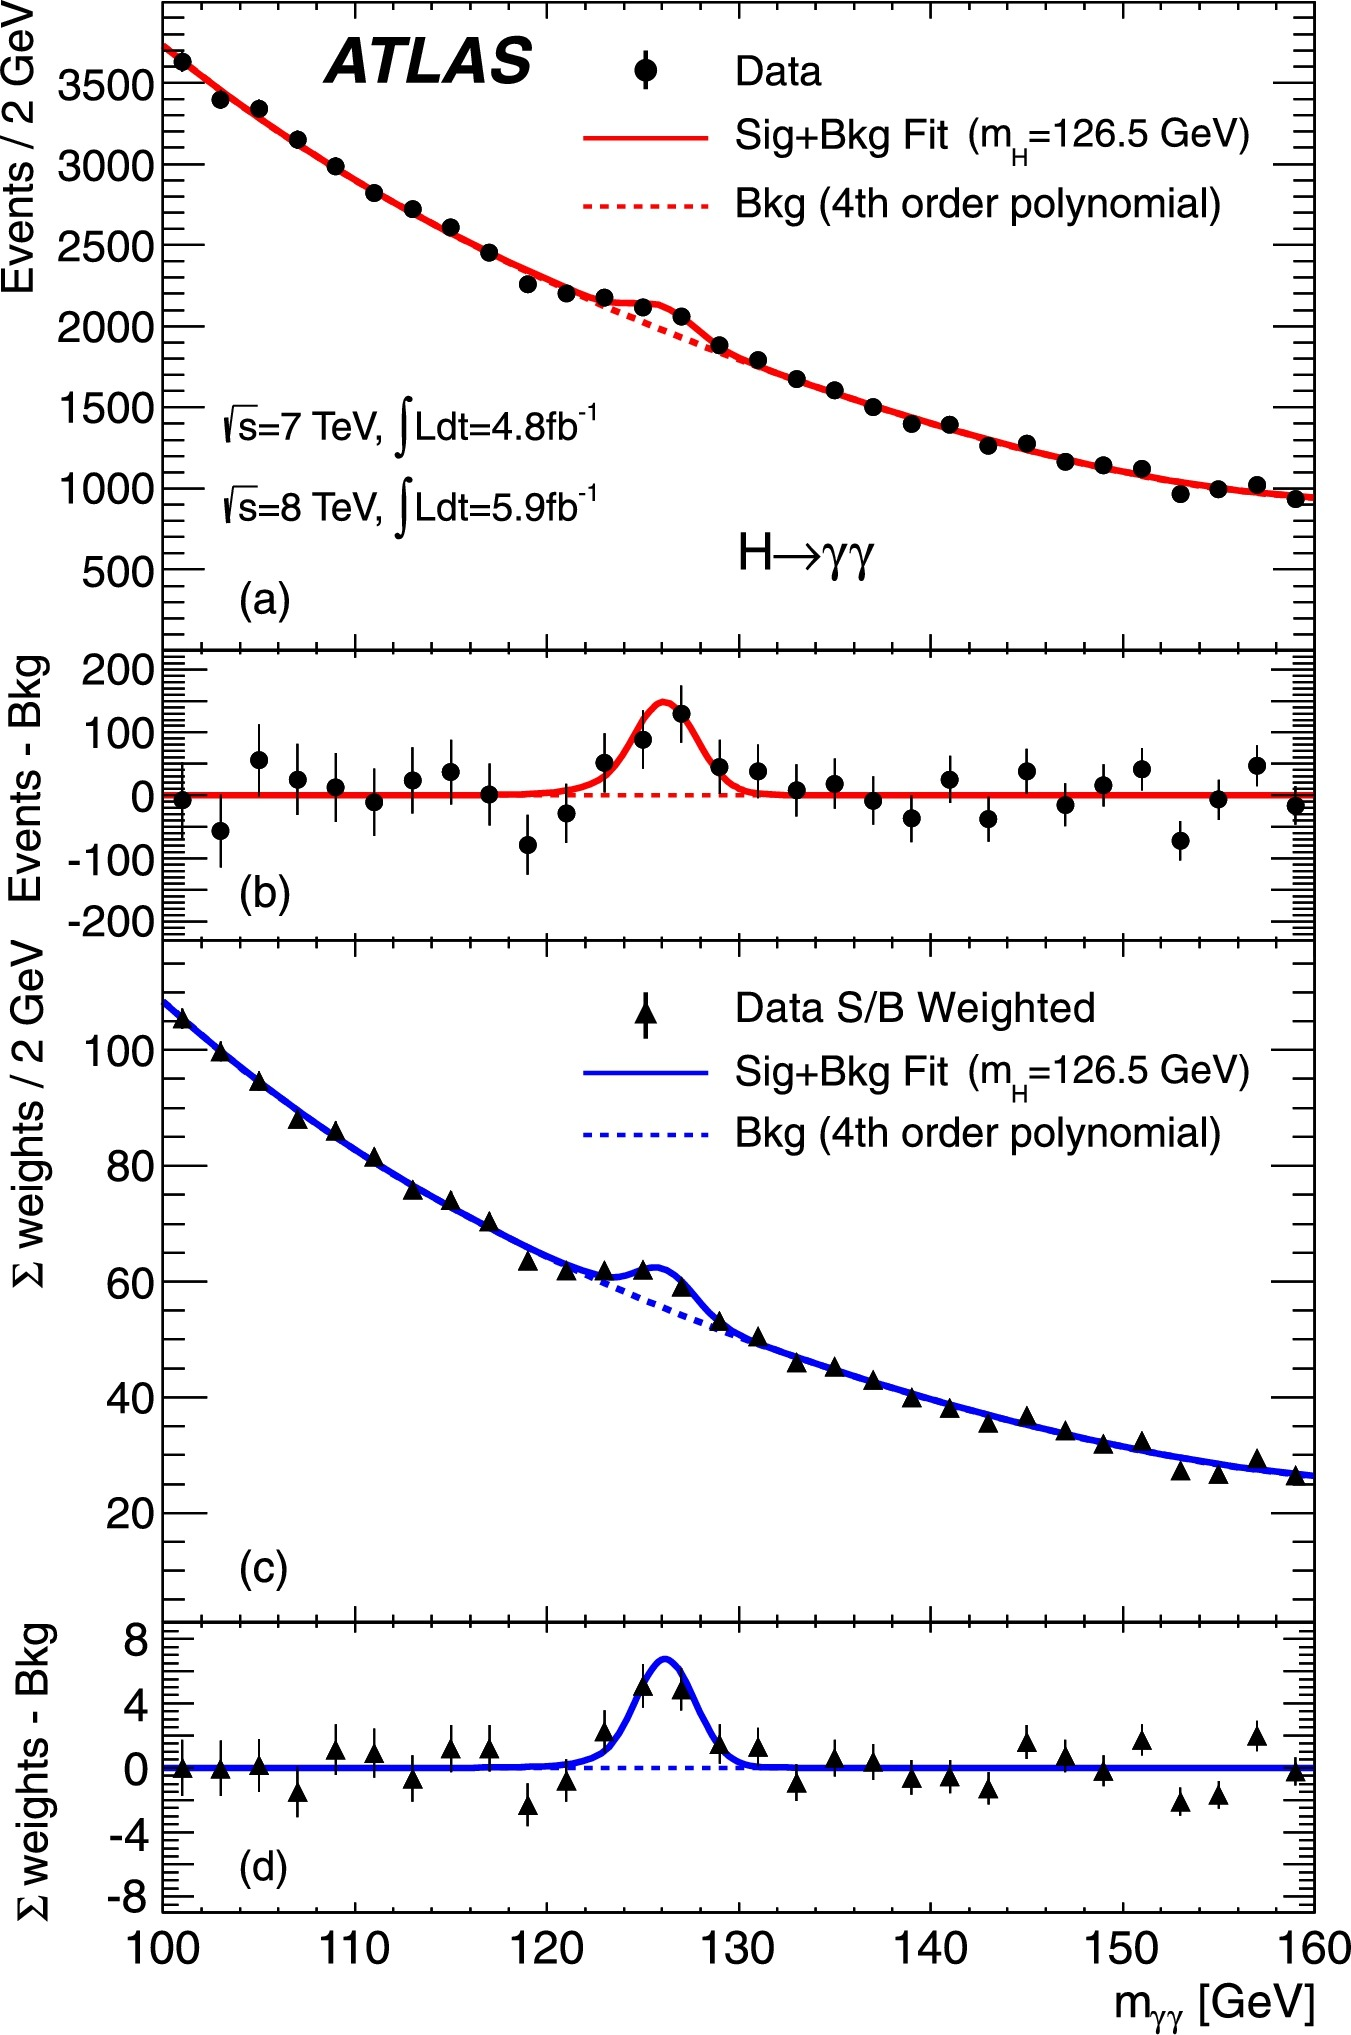
\includegraphics[width=.7\textwidth,keepaspectratio=true]{chapters/chapter2_theory/images/Higgs_Discovery_gam_gam.jpeg}
		% \caption{The distributions of the invariant mass of diphoton candidates after all selections for the combined 7 TeV and 8 TeV data sample. The inclusive sample is shown in (a) and a weighted version of the same sample in (c); the weights are explained in the text. The result of a fit to the data of the sum of a signal component fixed to $m_H=126.5$ GeV  and a background component described by a fourth-order Bernstein polynomial is superimposed. The residuals of the data and weighted data with respect to the respective fitted background component are displayed in (b) and (d). \cite{higgs-discovery-atlas}}
		% \label{fig:higgs-discovery}
		% \end{figure}
		\begin{figure}[!ht]
		\centering
		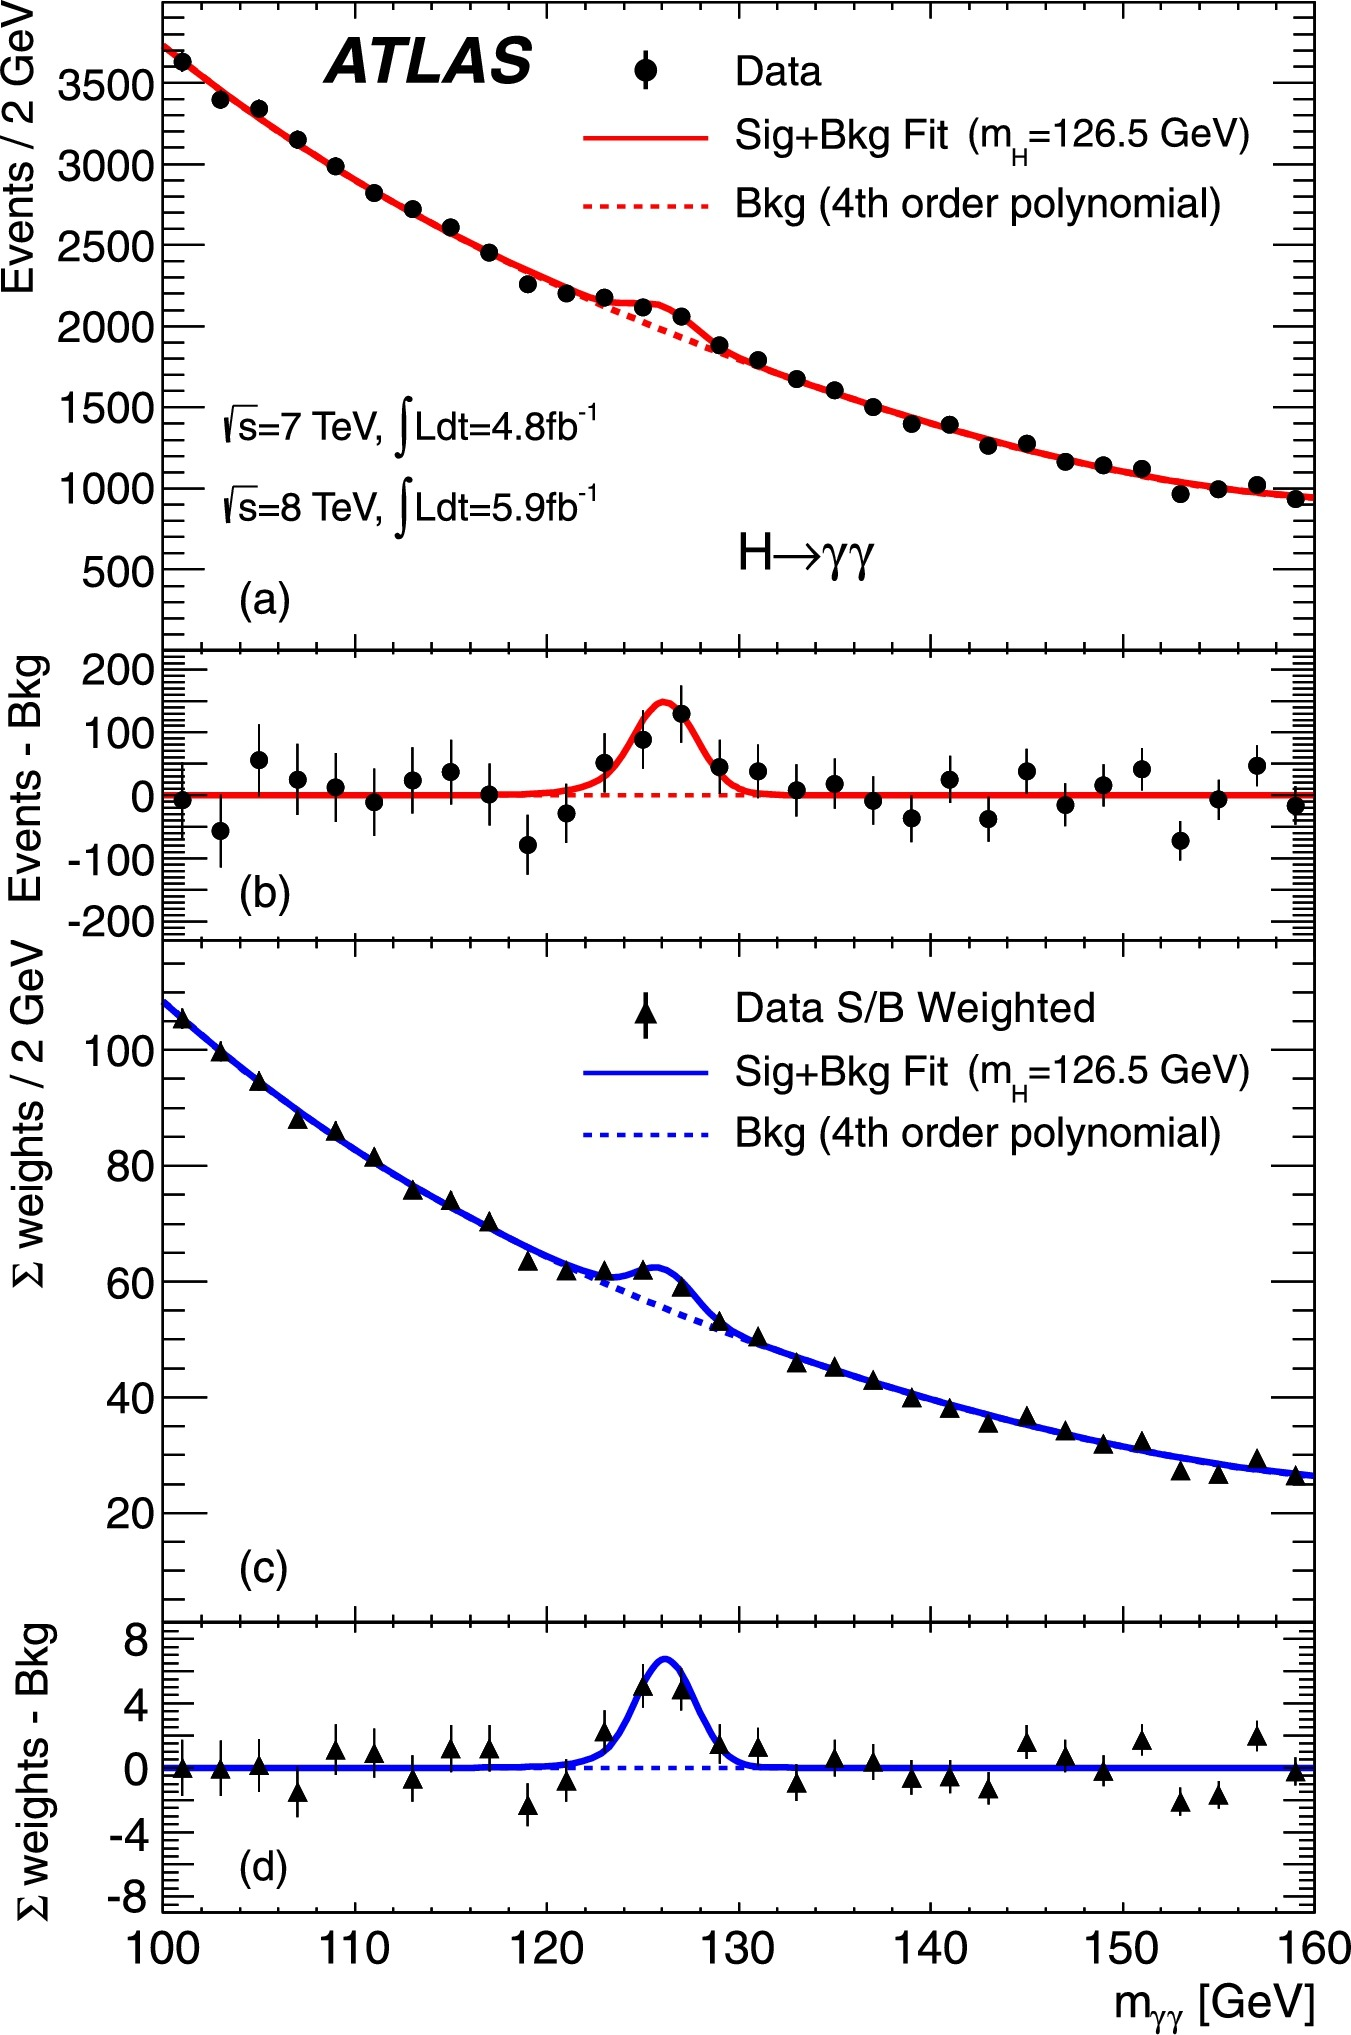
\includegraphics[width=.7\textwidth,keepaspectratio=true]{chapters/chapter2_theory/images/Higgs_Discovery_gam_gam.jpeg}
		\caption{The distributions of the invariant mass of diphoton candidates after all selections for the combined 7 TeV and 8 TeV data sample. The result of a fit to the data of the sum of a signal component fixed to $m_H=126.5$ GeV  and a background component described by a fourth-order Bernstein polynomial is superimposed. Taken from \cite{higgs-discovery-atlas}.}
		\label{fig:higgs-discovery}
		\end{figure}

\section{Supersymmetry}\label{sec:SUSY}
	While the \gls{SM} describes a wide range of physics to a high degree of accuracy, it is not without issues. For instance, the \gls{SM} does not offer an explanation for gravity, dark matter, or the observed matter-antimatter asymmetry of the universe. In addition, the \gls{SM} predicts the mass of neutrinos to be 0. Observed neutrino mixing, where $\nu_e \to \nu_\mu$, $\nu_\tau \to \nu_\mu$, etc., contradicts this; neutrinos must have mass \cite{pdg}.

	One promising model that offers solutions to many of these issues is \gls{SUSY}. As discussed previously, the \gls{SM} is built upon symmetries, and the breaking of these symmetries gives us electroweak unification. \gls{SUSY} proposes another symmetry, this time between fermions and bosons. 
	\begin{equation}\label{eqn:SUSY}
	\begin{split}
		Q | Fermion \rangle = | Boson \rangle, \\
		Q | Boson \rangle = | Fermion \rangle
	\end{split}
	\end{equation}
	Equation \ref{eqn:SUSY} shows how the \gls{SUSY} operator Q acts on particles. Here, Q provides a bosonic supersymmetric partner to every fermion and vice versa. \gls{SUSY} naturally offers solutions to the ``hierarchy problem'' with the \gls{SM}. 

	The hierarchy problem arises from the difference in electroweak ($M_W\sim100$ GeV)  and Planck ($M_P\sim2.4\, \mathrm{x} \, 10^{18}$ GeV) mass scales. For the Higgs mass to be on the scale of $M_H \sim 125$ GeV incredibly large and small mass terms must cancel perfectly, leading to a feeling of ``unnaturalness''. \gls{SUSY} brings many new particles into the picture, theorized to occupy the intermediate mass range leading to a more natural theory.

	\subsection{\acrlong{MSSM} Particles}\label{ssec:MSMM}
		\gls{SUSY} is a large group of theories that include theories with various numbers of additional superpartner particles. The \gls{MSSM} is the smallest extension of the \gls{SM} that introduces \gls{SUSY}. In the \gls{MSSM}\footnote{As well as all other \gls{SUSY} models.}, each \gls{SM} particle is part of a supermultiplet with its superpartner where both particles have the same quantum numbers, except spin. If this supersymmetry is unbroken, then the superpartner and the \gls{SM} particle would have the same mass as well. However, \gls{SUSY} has not been observed, so the supersymmetry must be broken putting the mass scale on the TeV scale. Table \ref{tab:MSSM} lists the \gls{MSSM} supermultiplets and the associated naming conventions.

			% \begin{table}[!thp]
			% 	\centering
			% 	\caption{\gls{SM} particles and their \gls{MSSM} partners \cite{pdg}.}
			% 	\begin{tabular}{| l | c | c |}
			% 	\hline
			% 	Name 				& \gls{SM} 	& \gls{MSSM} \\[1ex] \hline
			% 	\multicolumn{3}{|c|}{Spin-$\frac{1}{2}$ quarks and spin-$0$ squarks} \\[1ex] \hline
			% 	(s)up 				& $u$ 	& $\tilde{u}$ \\[1ex] \hline
			% 	(s)down 			& $d$ 	& $\tilde{d}$ \\[1ex] \hline
			% 	(s)charm 			& $c$ 	& $\tilde{c}$ \\[1ex] \hline
			% 	(s)strange 			& $s$		& $\tilde{s}$ \\[1ex] \hline
			% 	(s)top 				& $t$ 	& $\tilde{t}$ \\[1ex] \hline
			% 	(s)bottom 			& $b$ 	& $\tilde{b}$ \\[1ex] \hline
			% 	\multicolumn{3}{|c|}{Spin-$\frac{1}{2}$ leptons and spin-$0$ sleptons} \\[1ex] \hline
			% 	(s)electron 		& $e$ 	& $\tilde{e}$ \\[1ex] \hline
			% 	(s)electron (s)neutrino 	& $\nu_e$ 	& $\widetilde{\nu_e}$ \\[1ex] \hline
			% 	(s)muon 			& $\mu$ 	& $\tilde{\mu}$ \\[1ex] \hline
			% 	(s)muon (s)neutrino & $\nu_\mu$ 	& $\widetilde{\nu_\mu}$ \\[1ex] \hline
			% 	(s)tau 				& $\tau$ 	& $\tilde{\tau}$ \\[1ex] \hline
			% 	(s)tau (s)neutrino 	& $\nu_\tau$ 	& $\widetilde{\nu_\tau}$ \\[1ex] \hline
			% 	\multicolumn{3}{|c|}{Spin-$0$ Higgs and spin-$\frac{1}{2}$ Higgsinos} \\[1ex] \hline
			% 	Higgs(ino)			& $H$ 	& $\tilde{H}$ \\[1ex] \hline
			% 	gluon (gluino) 		& $g$ 	& $\tilde{g}$ \\[1ex] \hline
			% 	W (Wino) 			& $W^{\pm}$, $W^0$ & $\widetilde{W^\pm}, \widetilde{W^0}$ \\[1ex] \hline
			% 	B (Bino) 			& $B^0$ & $\widetilde{B^0}$ \\[1ex] \hline

 		% 		\end{tabular}
			% 	\label{tab:MSSM}
			% \end{table}

			\begin{table}[!thp]
				\centering
				\caption{\gls{SM} particles and their \gls{MSSM} partners \cite{pdg}.}
				\begin{tabular}{| c | c |}
				\hline
				\gls{SM} 	& \gls{MSSM} \\[1ex] \hline
				\multicolumn{2}{|c|}{Spin-$\frac{1}{2}$ quarks and spin-$0$ squarks ($\times 3$ generations)} \\[1ex] \hline
				$(u_{L} \, d_{L})$ 					& $(\tilde{u}_{L} \, \tilde{d}_{L})$ \\[1ex]
				$u^{\dagger}_{R}$ 					& $\bar{u}^{*}_{R}$ \\[1ex]
				$d^{\dagger}_{R}$ 					& $\bar{d}^{*}_{R}$ \\[1ex] 
				\hline \hline

				\multicolumn{2}{|c|}{Spin-$\frac{1}{2}$ leptons and spin-$0$ sleptons ($\times 3$ generations)} \\[1ex] \hline
				${\nu_{L} \, e_{L}}$ 				& $(\tilde{\nu}_{L} \,  \tilde{e}_{L}$ \\[1ex]
				$e^{\dagger}_{R}$ 					& $\bar{e}^{*}_{R}$ \\[1ex]

				\hline \hline
				\multicolumn{2}{|c|}{Spin-$0$ Higgs and spin-$\frac{1}{2}$ Higgsinos} \\[1ex] \hline
				$(H^{\dagger}_{u} 	\, H^{0}_{u})$ 	& $(\tilde{H}^{+}_{u} \, \tilde{H}^{0}_{u} )$ \\[1ex]
				$(H^{0}_{d} 		\, H^{-}_{d})$ 	& $(\tilde{H}^{0}_{d} \, \tilde{H}^{-}_{d} )$ \\[1ex]

				\hline \hline
				\multicolumn{2}{|c|}{Spin-$1$ gauge bosons and spin-$\frac{1}{2}$ gauginos} \\[1ex] \hline
				$g$									& $\tilde{g}$ \\[1ex]
				$(W^{\pm} \, W^{0})$ 				& $(\tilde{W}^{\pm} \, \tilde{W}^{0})$ \\[1ex]
				$B^{0}$ 							& $\tilde{B}^{0}$ \\[1ex]
				\hline \hline

 				\end{tabular}
				\label{tab:MSSM}
			\end{table}


	\subsection{2 Higgs Doublet Model}\label{ssec:2HDM}
		Having only one Higgs chiral supermultiplet with hypercharge $Y_W=\pm \frac{1}{2}$ leads to a gauge anomaly \cite{2HDM}. This can be resolved by introducing two Higgs doublets with hypercharge $Y_W=\frac{1}{2}$ and $Y_W=-\frac{1}{2}$. Such is the case in the \gls{MSSM} which requires two complex doublet scalar fields where one couples to the up-type quarks and the other couples to down-type quarks and charged leptons. The \gls{MSSM} Higgs sector has 8 degrees of freedom. Following the same type of mechanism described in Section \ref{ssec:Higgs} three of these degrees of freedom give the observed $W^\pm$ and $Z^0$ bosons. 
		\begin{table}[!thp]
				\centering
				\caption{\gls{2HDM} extended Higgs sector \cite{2HDM}}
				\begin{tabular}{| l | c |}
				\hline
				light neutral scalar 	& $h^0$ \\ \hline
				heavy neutral scalar 	& $H^0$ \\ \hline
				neutral pseudoscalar 	& $A^0$ \\ \hline
				two charged scalars 	& \Hpm \\ \hline
 				\end{tabular}
				\label{tab:2HDM}
		\end{table}
		This leaves the extended Higgs sector shown in Table \ref{tab:2HDM}, where the $h^0$ is a SM-like Higgs. The boson discovered by the \gls{ATLAS} and \gls{CMS} collaborations in 2012 is consistent with the $h^{0}$. When referring to the charged Higgs bosons, we often refer to them using one symbol \Hpm. In the \gls{2HDM} there are two free parameters\footnote{There are more free parameters with regards to the full \gls{2HDM}. These are the two regarding the charged Higgs bosons that are relevant for the rest of this dissertation.}, the masses of the \Hpm and the ratio of their vacuum expectation values which is defined as \tanb. At the time of writing, the extended Higgs sector is an active area of research with many new searches actively being performed \cite{pdg}. The most recent results from ATLAS can be seen in Reference \cite{ATLAS-HBSM-Summary}.

		% These types of models are referred to as Type II \gls{2HDM} \cite{2HDM}.


\section{Charged Higgs Bosons}\label{sec:Hpm}
	Since the \Hpm couplings are proportional to the fermion masses, the main production modes at the LHC are through \ttbar and $Wt$ diagrams where the $W^{\pm}$ boson is replaced by a \Hpm.
	\begin{figure}[!ht]
		\centering
		\subfloat[\label{fig:hpm-diagrams_a}]{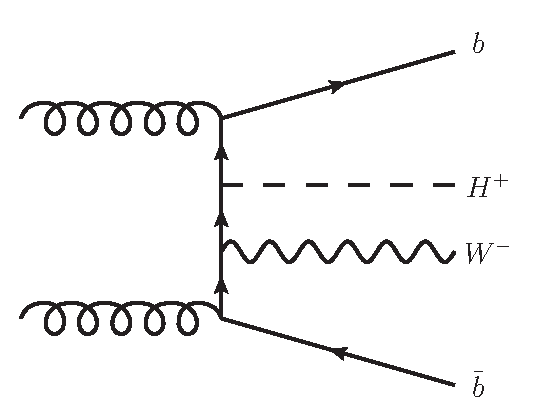
\includegraphics[width=0.3\textwidth]{chapters/chapter2_theory/images/NonResonant.pdf}}
		\subfloat[\label{fig:hpm-diagrams_b}]{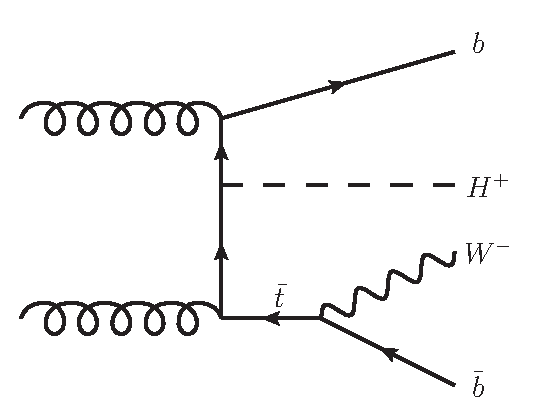
\includegraphics[width=0.3\textwidth]{chapters/chapter2_theory/images/SingleResonant.pdf}}
		\subfloat[\label{fig:hpm-diagrams_c}]{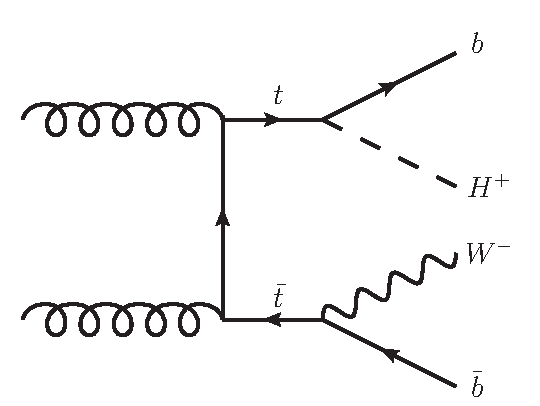
\includegraphics[width=0.3\textwidth]{chapters/chapter2_theory/images/DoubleResonant.pdf}}
		\caption{\label{fig:hpm-diagrams} Examples of leading-order Feynman diagrams contributing to the production of charged Higgs bosons in $pp$ collisions: (a) non-resonant top-quark production prevalent in the intermediate-mass range, (b) single-resonant top-quark production that dominates at large \Hpm masses, (c) double-resonant top-quark production that dominates at low \Hpm masses. The interference between these three diagrams becomes most relevant in the intermediate-mass region.}
	\end{figure}
	\begin{figure}[!ht]
		\centering
		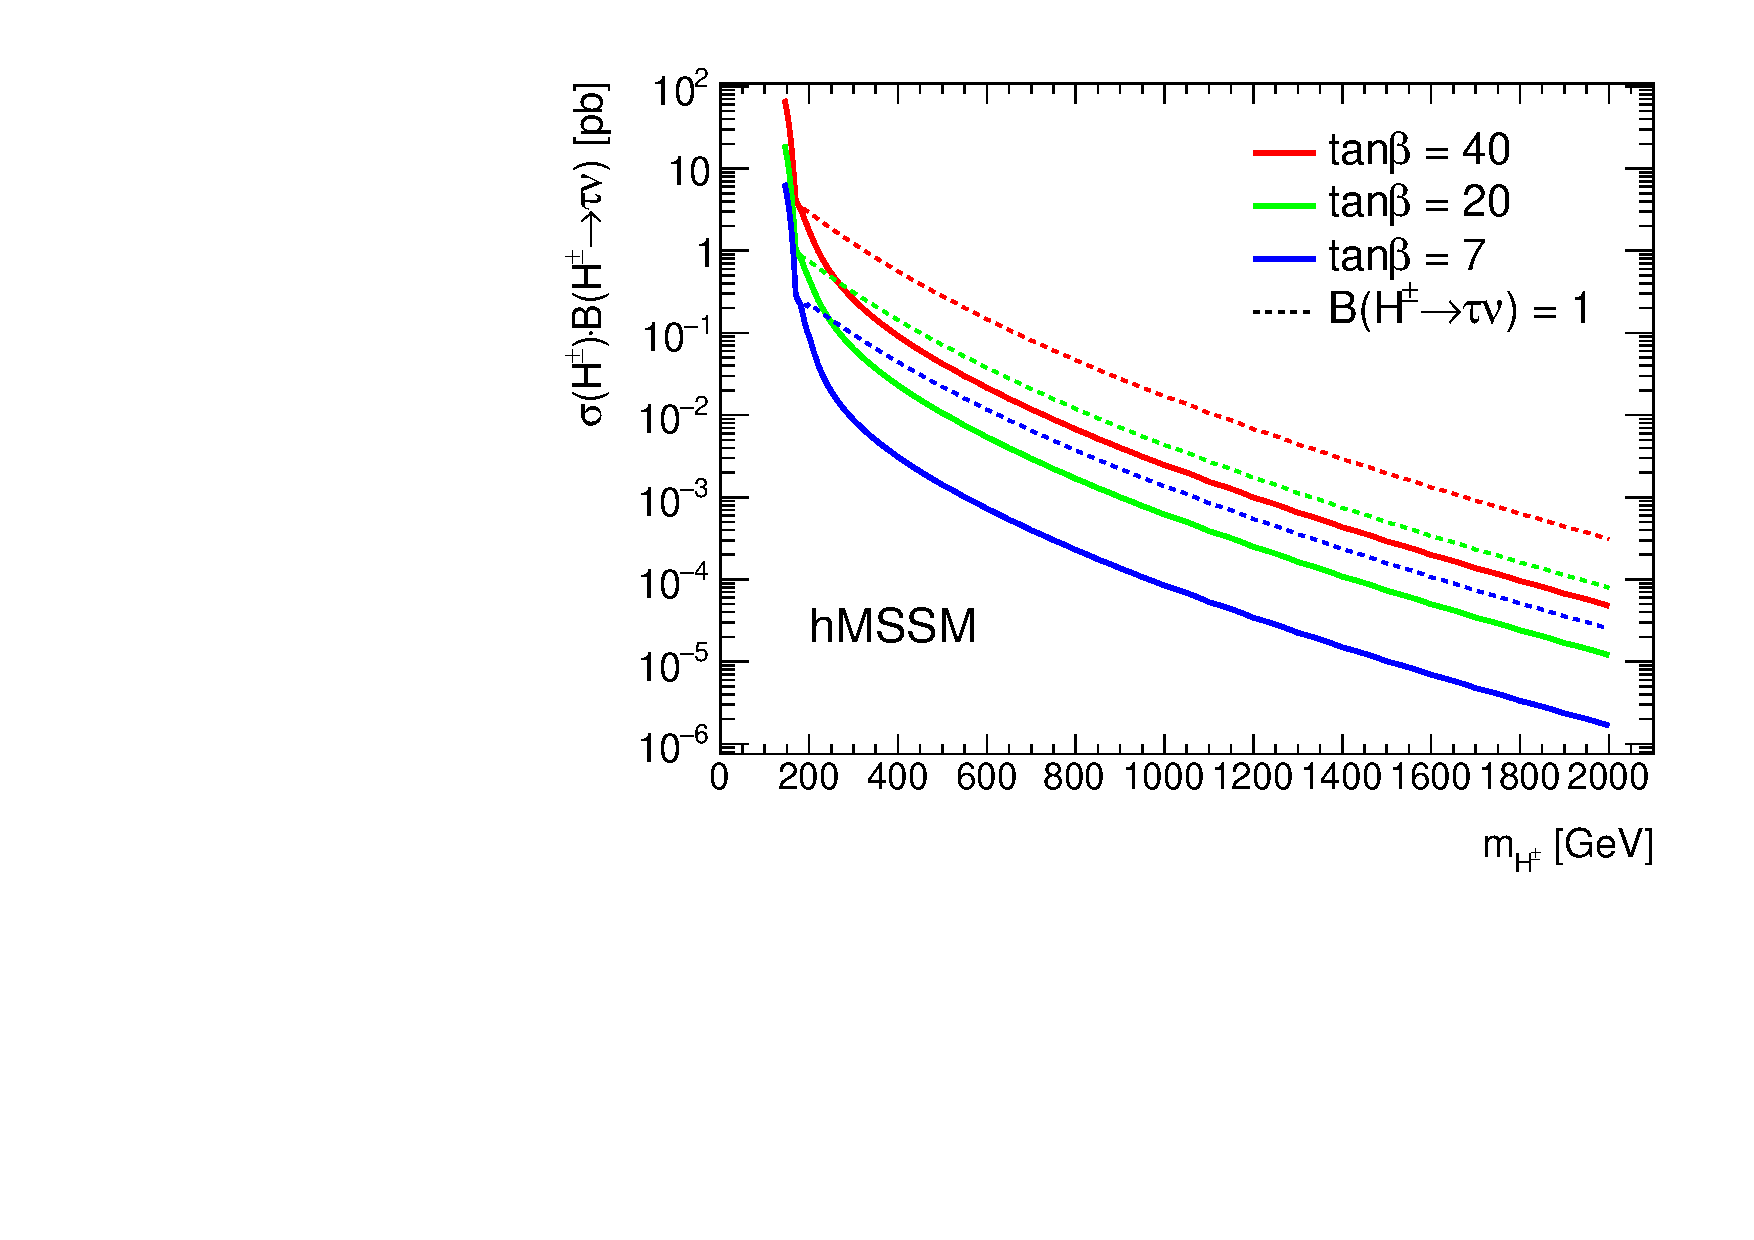
\includegraphics[width=0.75\textwidth]{chapters/chapter2_theory/images/XSBR_hmssm.pdf}
		\caption{\label{fig:hpm-xsec} Variation of $\sigma(\pp \to tb\Hpm) \times B(\HpmLong)$ with the charged Higgs boson mass in \pp collisions at \sqs, for \tanb values of 7, 20, and 40 in the hMSSM scenario. Dashed lines correspond to $B(\HpmLong)$ set to 1, hence they show the dependence of $\sigma(\pp \to tb\Hpm)$ with \mHpm. \cite{hpm-previous} }
	\end{figure}
	The production diagrams considered in this dissertation can be seen in figure \ref{fig:hpm-diagrams}. The cross section at various \tanb values can be seen as a function of \mHpm in figure \ref{fig:hpm-xsec}. The cross section scales with \tanb and at very small values the top Yukawa couplings become non-perturbative, meaning they are very difficult to predict and very unlikely to occur. In this dissertation the decay channel considered is \HpmLong. 
	\begin{figure}[!ht]
		\centering
		\subfloat[\label{fig:hpm-br_a}]{\includegraphics[width=0.5\textwidth]{chapters/chapter2_theory/images/YRHXS3_BR_fig33.eps}}
		\subfloat[\label{fig:hpm-br_b}]{\includegraphics[width=0.5\textwidth]{chapters/chapter2_theory/images/YRHXS3_BR_fig34.eps}}
		\caption{\label{fig:hpm-br} Branching fractions of \Hpm as a function of \mHpm for (a) $\tanb = 10$ and (b) $\tanb = 50$ in the $m^{mod+}_{h}$ scenario of the \gls{MSSM} \cite{Higgs-Crosssections}. }
	\end{figure}
	As can be seen in Figure \ref{fig:hpm-br}, the \HpmLong decay channel is especially relevant at low \mHpm and high \tanb. This dissertation describes a search for charged Higgs bosons produced in association with a top quark, where only the \HpmLong decay channel is considered. Other decay modes of the \Hpm to \gls{SM} particles are covered in other searches \cites{MSSM-benchmarks}. Decay channels of \Hpm to other \gls{MSSM} are not considered in this dissertation. The search consists of two sub-channels, \taujets and \taulep, where the associated top quark decays either hadronically or leptonically respectively. 

	Within the \gls{MSSM}, several benchmarks are defined taking into account higher-order corrections and keeping the number of free parameters in the model small \cite{MSSM-benchmarks}. Figure \ref{fig:hpm-xsec} is made assuming the hMSSM model, where $h^0$ is taken as the observed 125 GeV Higgs and the absence of observed \gls{SUSY} at the LHC is taken into account by setting the \gls{SUSY} scale to $M_{SUSY}>1$ TeV \cite{hMSSM}. Figure \ref{fig:hpm-br} shows the branching ratios of \Hpm for various \tanb values in the $m^{mod+}_{h}$ model where the benchmark scenario $m^{max}_{h}$\footnote{The $m^{max}_{h}$ scenario is constructed to yield the highest possible mass for h at any given \tanb.} has been modified to interpret $h$ as the observed boson \cite{MSSM-benchmarks}.

	\subsection{Previous Result}\label{ssec:Prev Hpm}
		To add context to this dissertation, it is important to reference the results of the previous iteration of the search discussed in this dissertation\footnote{The author joined the analysis team towards the end of this iteration and performed some validation studies.}. The \gls{ATLAS} collaboration published a paper in 2018 covering the data taking years of 2015 and 2016 \cite{hpm-previous}, whereas this dissertation covers the full Run-2 (2015-2018) dataset. 
		\begin{figure}[!ht]
			\centering
			\subfloat[\label{fig:hpm-prev-limits_a}]{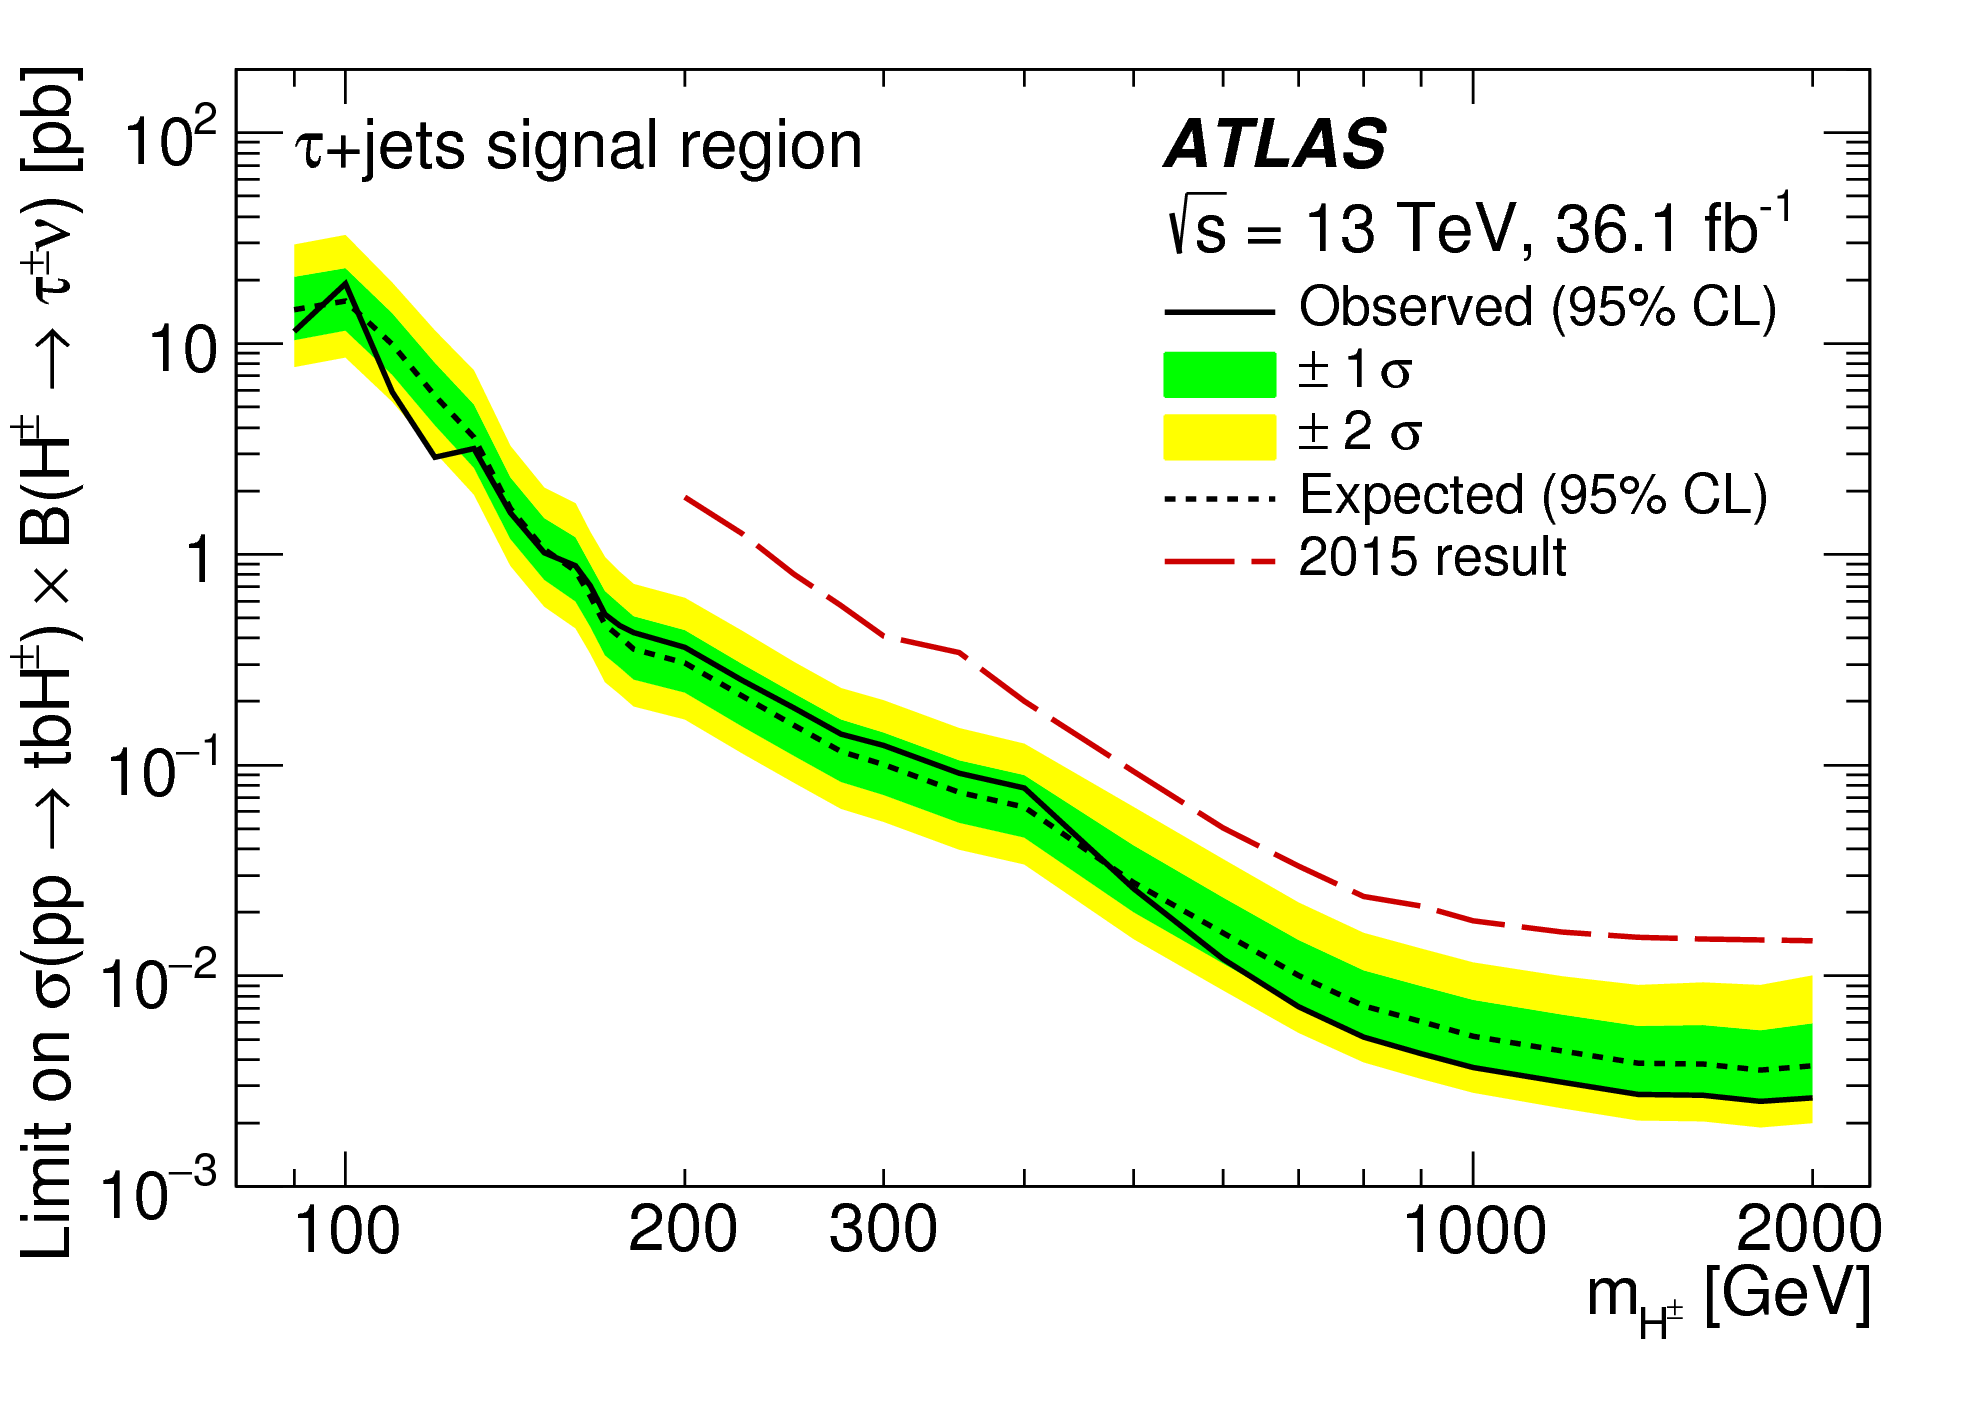
\includegraphics[width=0.5\textwidth]{chapters/chapter2_theory/images/Previous_Limits_Taujets.png}}
			\subfloat[\label{fig:hpm-prev-limits_b}]{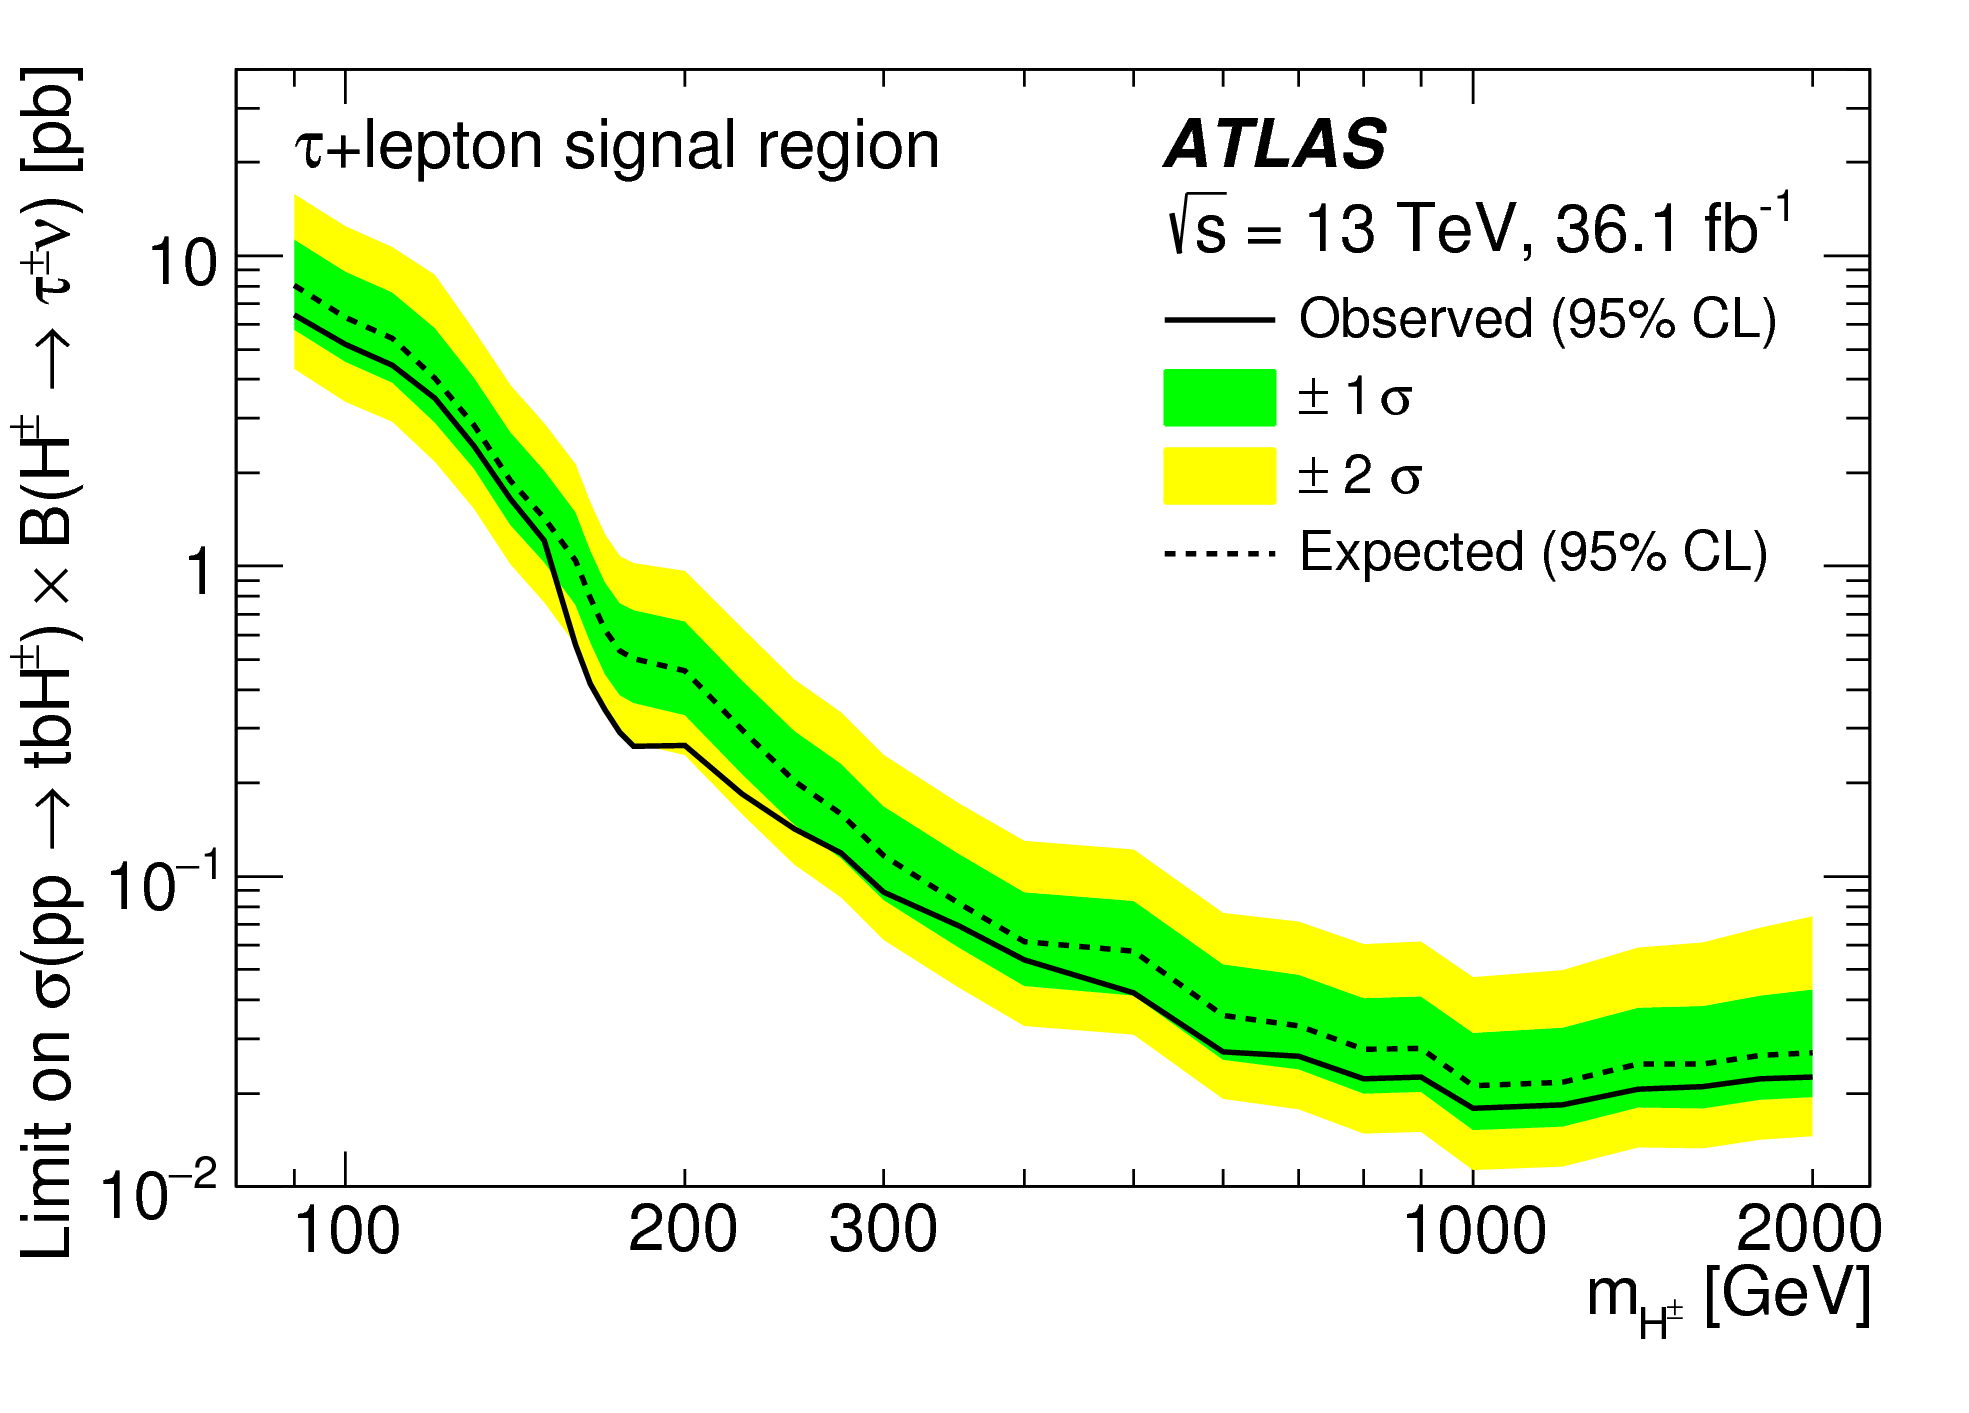
\includegraphics[width=0.5\textwidth]{chapters/chapter2_theory/images/Previous_Limits_Taulep.png}} \\
			\subfloat[\label{fig:hpm-prev-limits_c}]{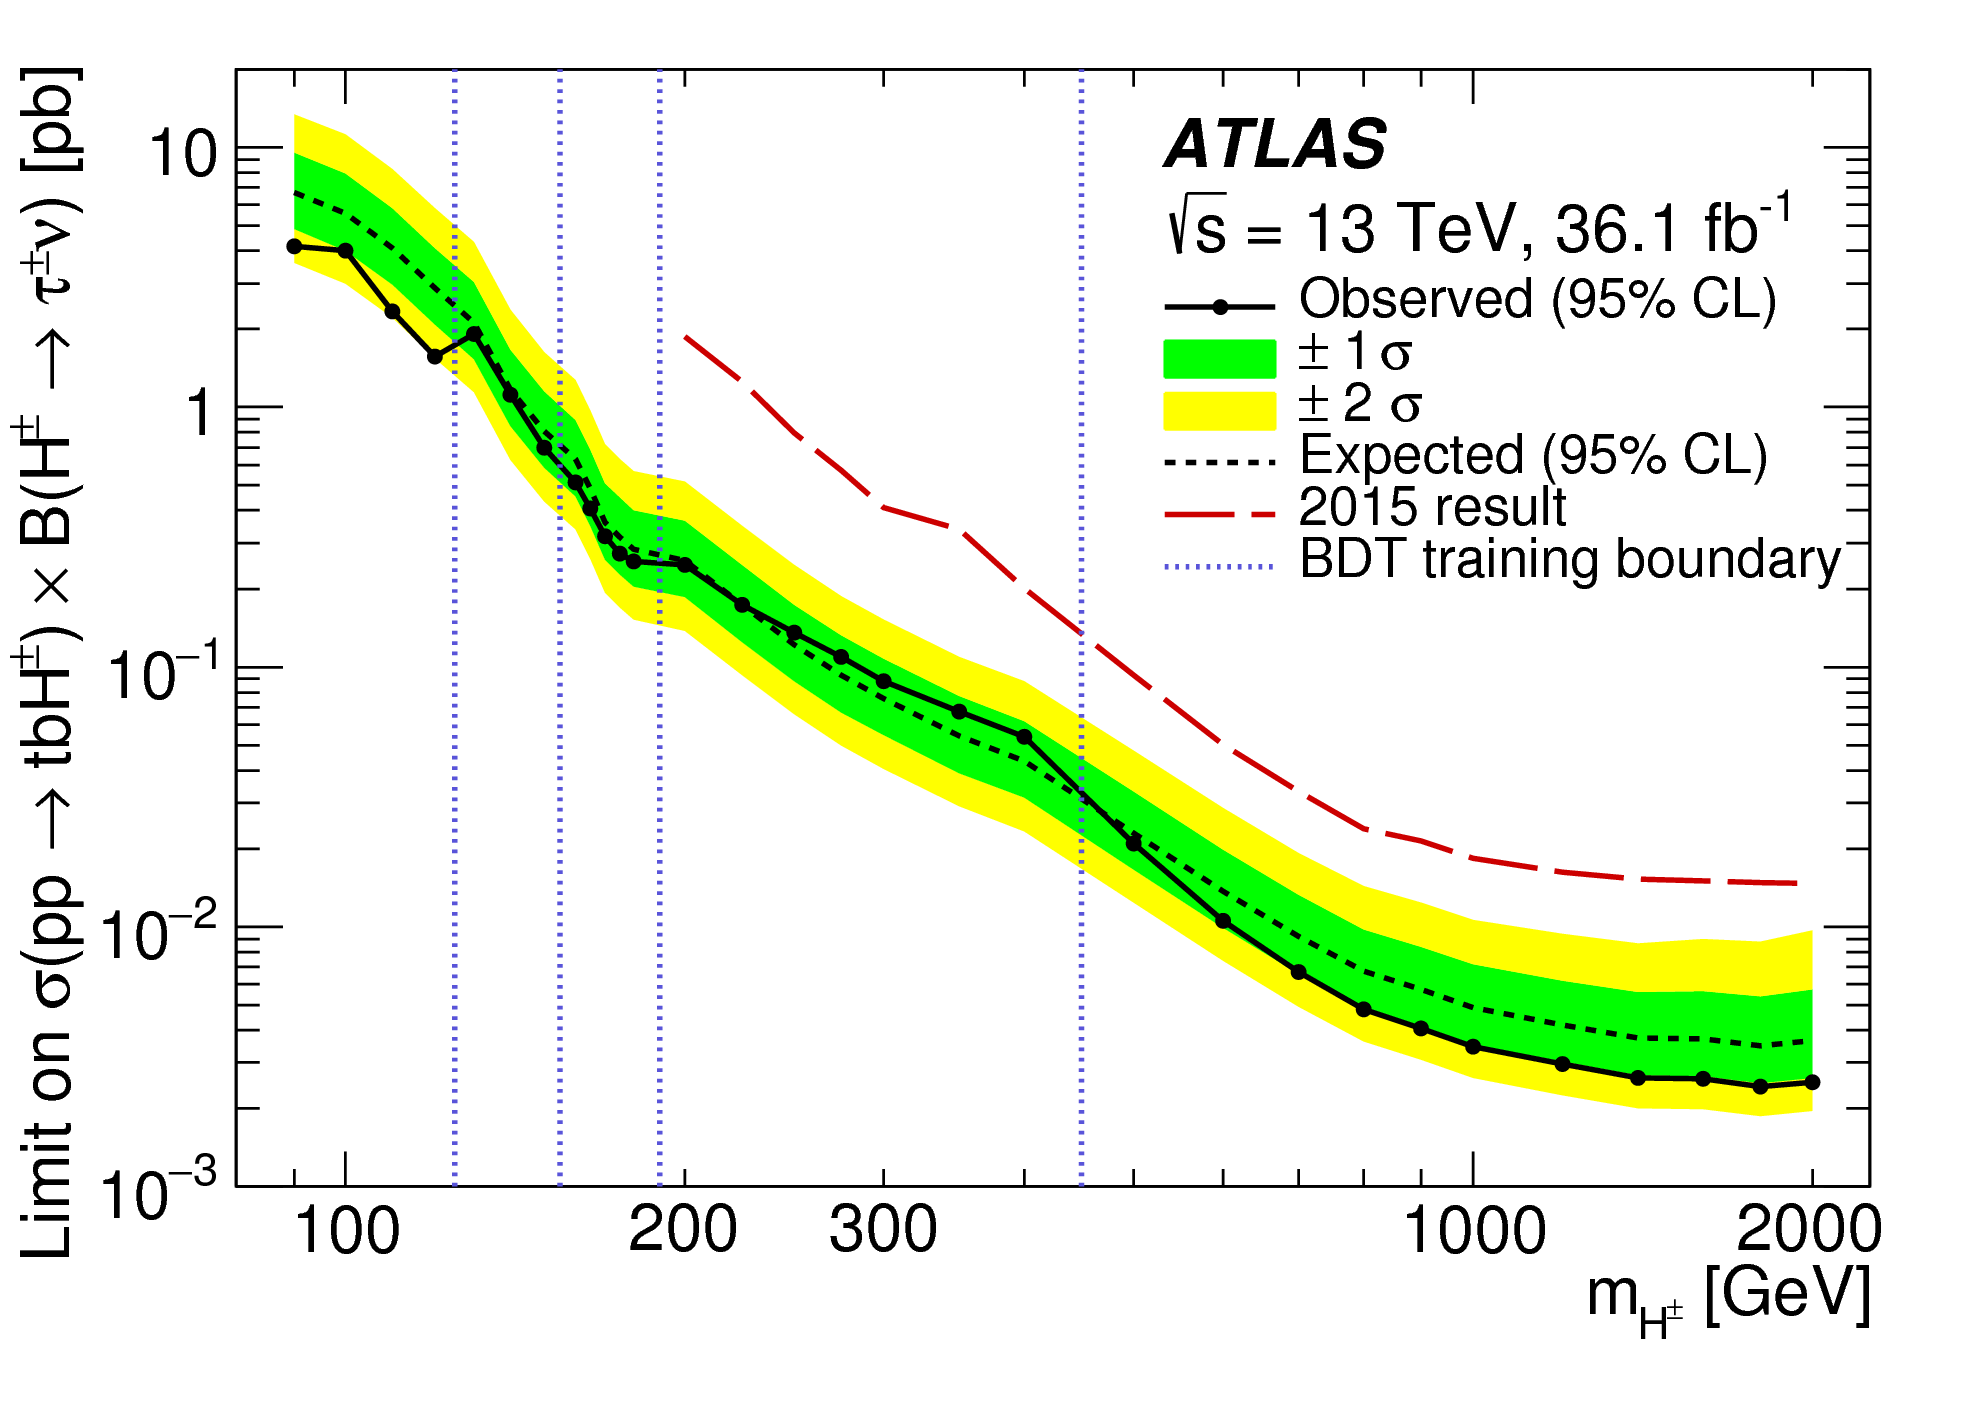
\includegraphics[width=0.75\textwidth]{chapters/chapter2_theory/images/Previous_Limits_Combined.png}}
			\caption{\label{fig:hpm-prev-limits} Exclusion limits at 95\% CL on $\sigma(pp \to tbH^{\pm} \times B(H^{\pm} \to \tau^\pm \nu)) [pb]$. Top left (a) shows the \taujets subchannel, top right (b) corresponds to the \taulep subchannel and bottom (c) shows the combination of the two subchannels. Taken from Reference \cite{hpm-previous}. }
		\end{figure}
		\begin{figure}[!ht]
			\centering
			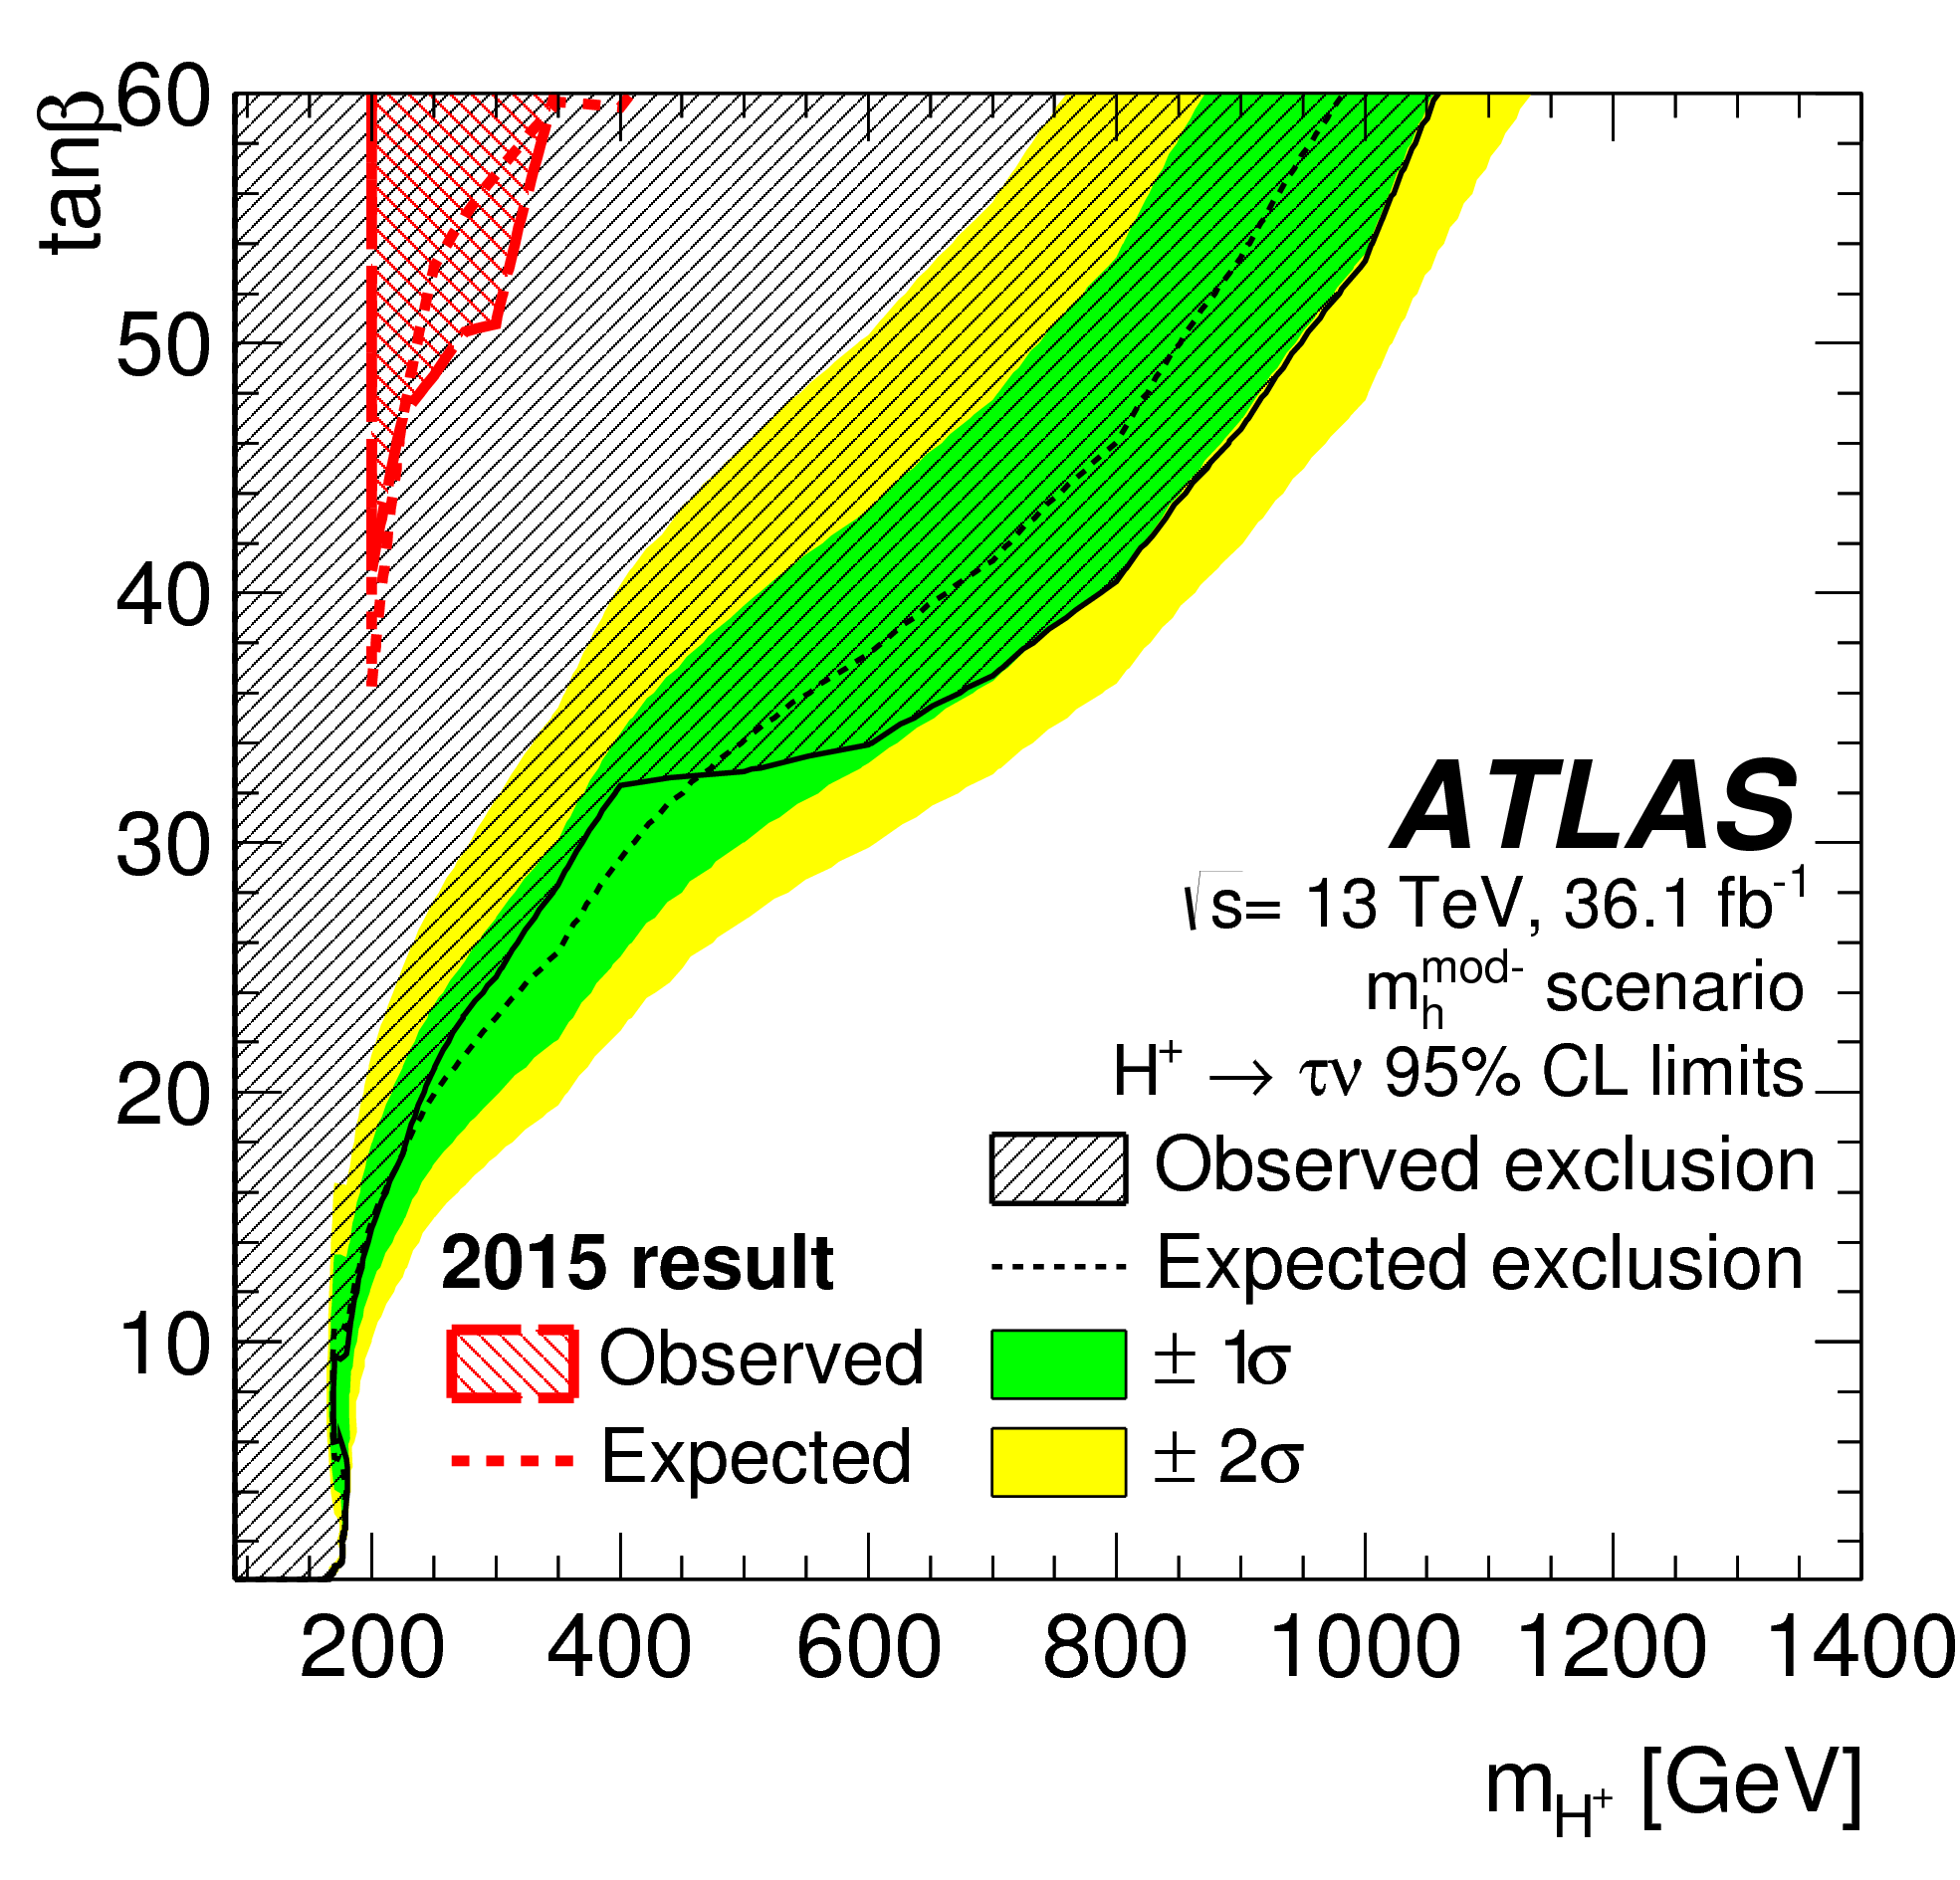
\includegraphics[width=0.75\textwidth]{chapters/chapter2_theory/images/Previous_Limits_Combined_tanb.png}
			\caption{\label{fig:hpm-prev-limits-tanb} Exclusion limits at 95\% CL on \tanb as a function of \mHpm \cite{hpm-previous}. }
		\end{figure}
		Figure \ref{fig:hpm-prev-limits} shows the limits on the cross section and Figure \ref{fig:hpm-prev-limits-tanb} shows the limits on \tanb as a function of \mHpm. 

		There are many other searches for charged Higgs bosons that have been performed by several experiments in many different decay channels. Figure \ref{fig:hpm-taunu-cms-limits} shows the results from CMS in the same \HpmLong decay channel \cite{CMS-taunu}. Figure \ref{fig:hpm-tb-limits} shows the ATLAS results for a charged Higgs search in the $\Hpm \to tb$ decay channel and Figure \ref{fig:hpm-tb-tanb-limits} shows the previous \HpmLong search results overlayed on the $\Hpm \to tb$ results in two theoretical models \cite{Hpm-to-tb}.

		\begin{figure}[!ht]
			\centering
			\subfloat[\label{fig:hpm-taunu-cms-limits_a}]{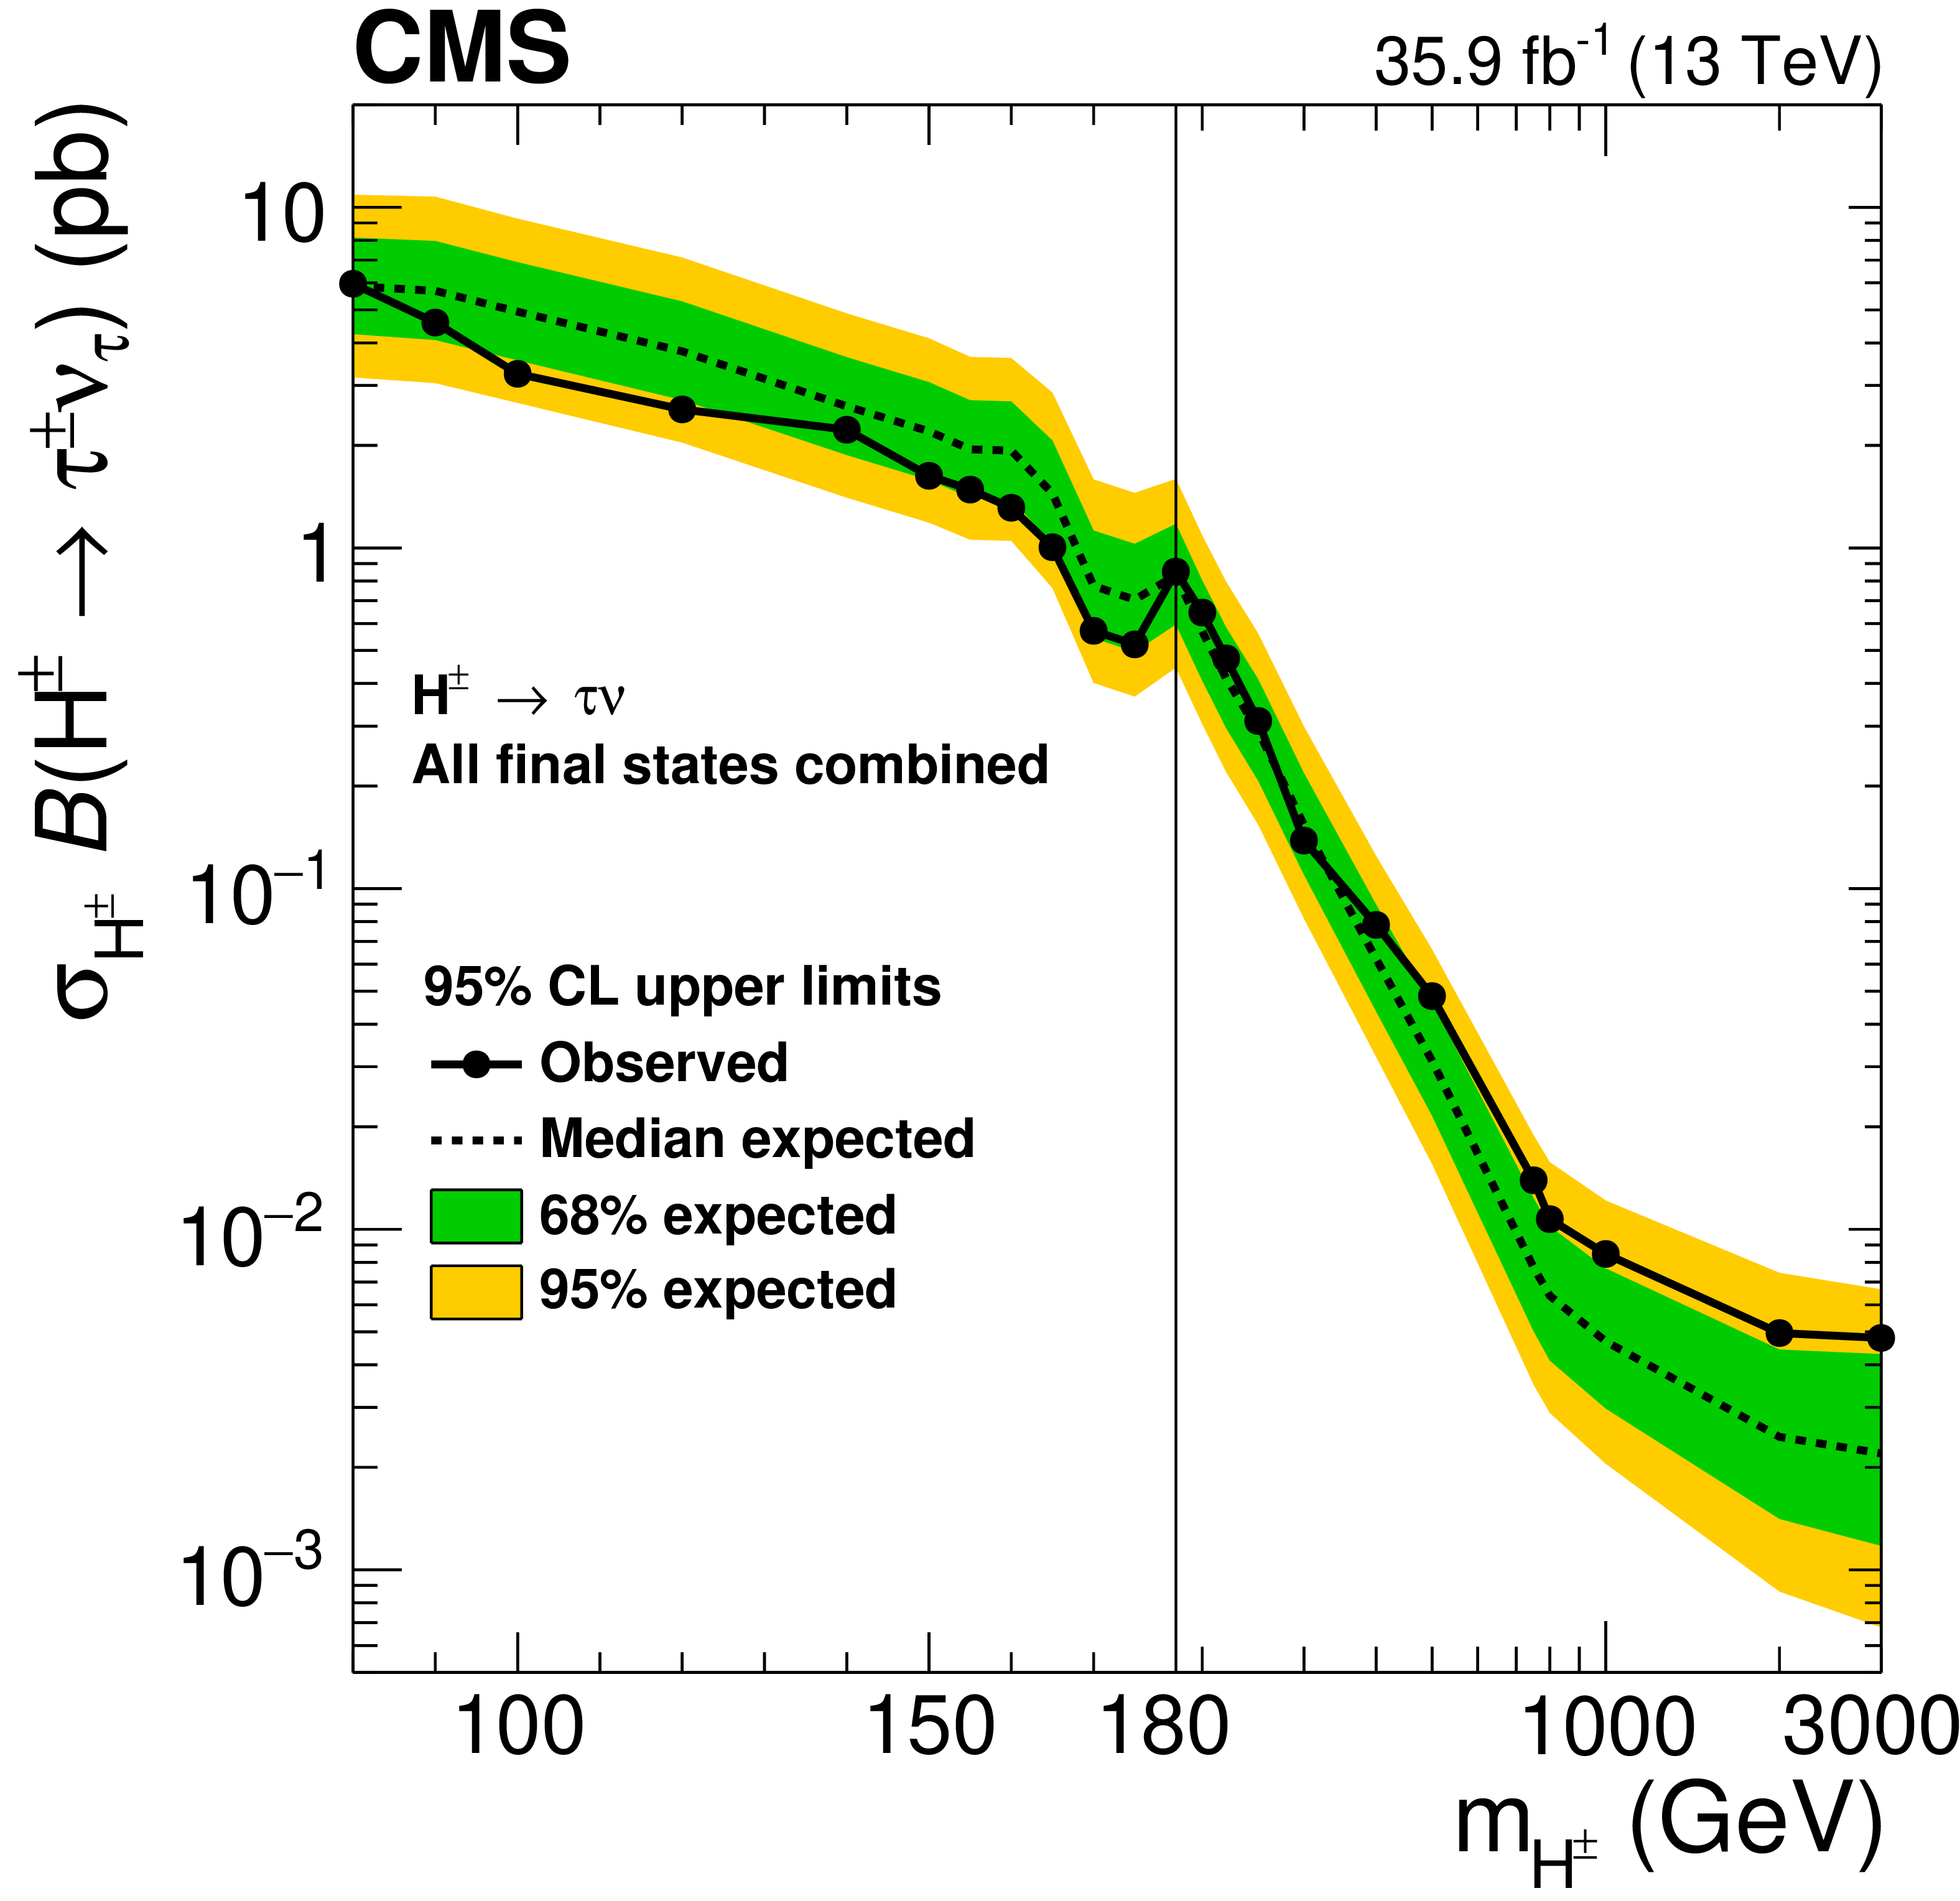
\includegraphics[width=0.5\textwidth,keepaspectratio=true]{chapters/chapter2_theory/images/CMS_taunu_xsec_limits.png}}
			\subfloat[\label{fig:hpm-taunu-cms-limits_b}]{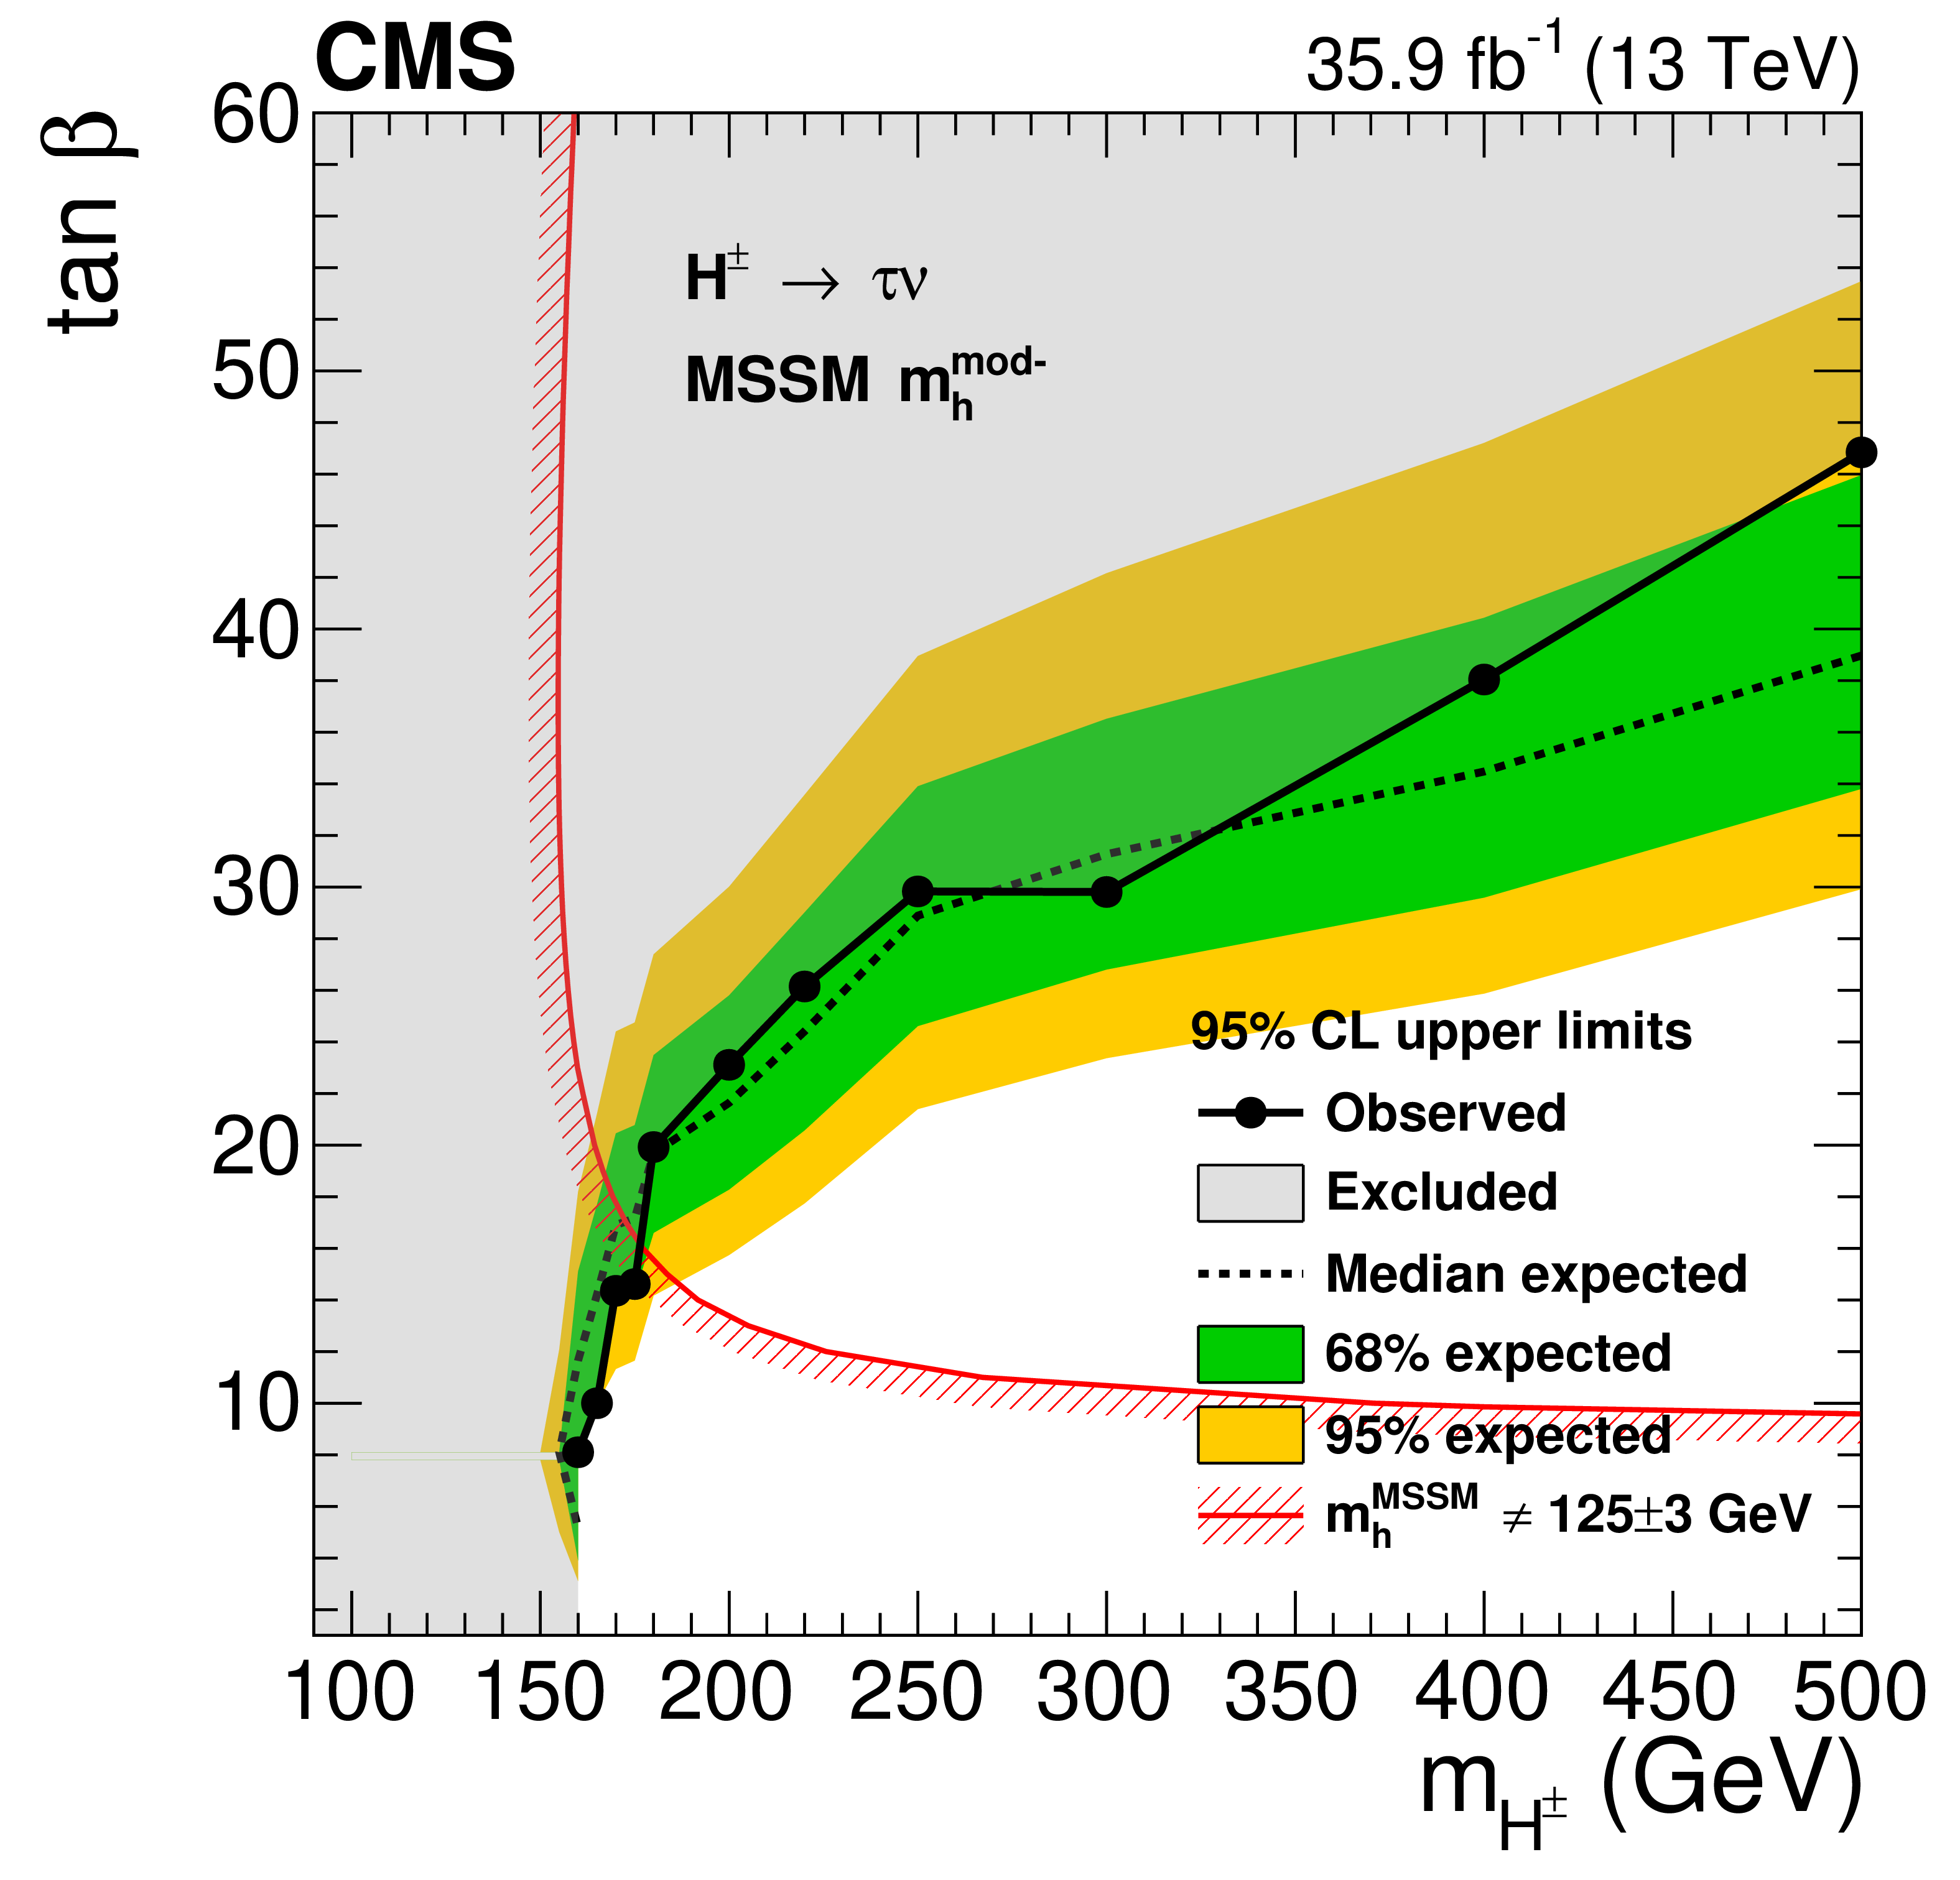
\includegraphics[width=0.5\textwidth,keepaspectratio=true]{chapters/chapter2_theory/images/CMS_taunu_tanb_limits.png}}
			\caption{\label{fig:hpm-taunu-cms-limits} (a) Exclusion limits at 95\% CL on $\sigma_{\Hpm} B(\Hpm \to \tau^\pm \nu_{\tau}) [pb]$ from the CMS collaboration \cite{CMS-taunu}. (b) Exclusion limits at 95\% CL on \tanb and \mHpm \cite{CMS-taunu}. }
		\end{figure}

		\begin{figure}[!ht]
			\centering
			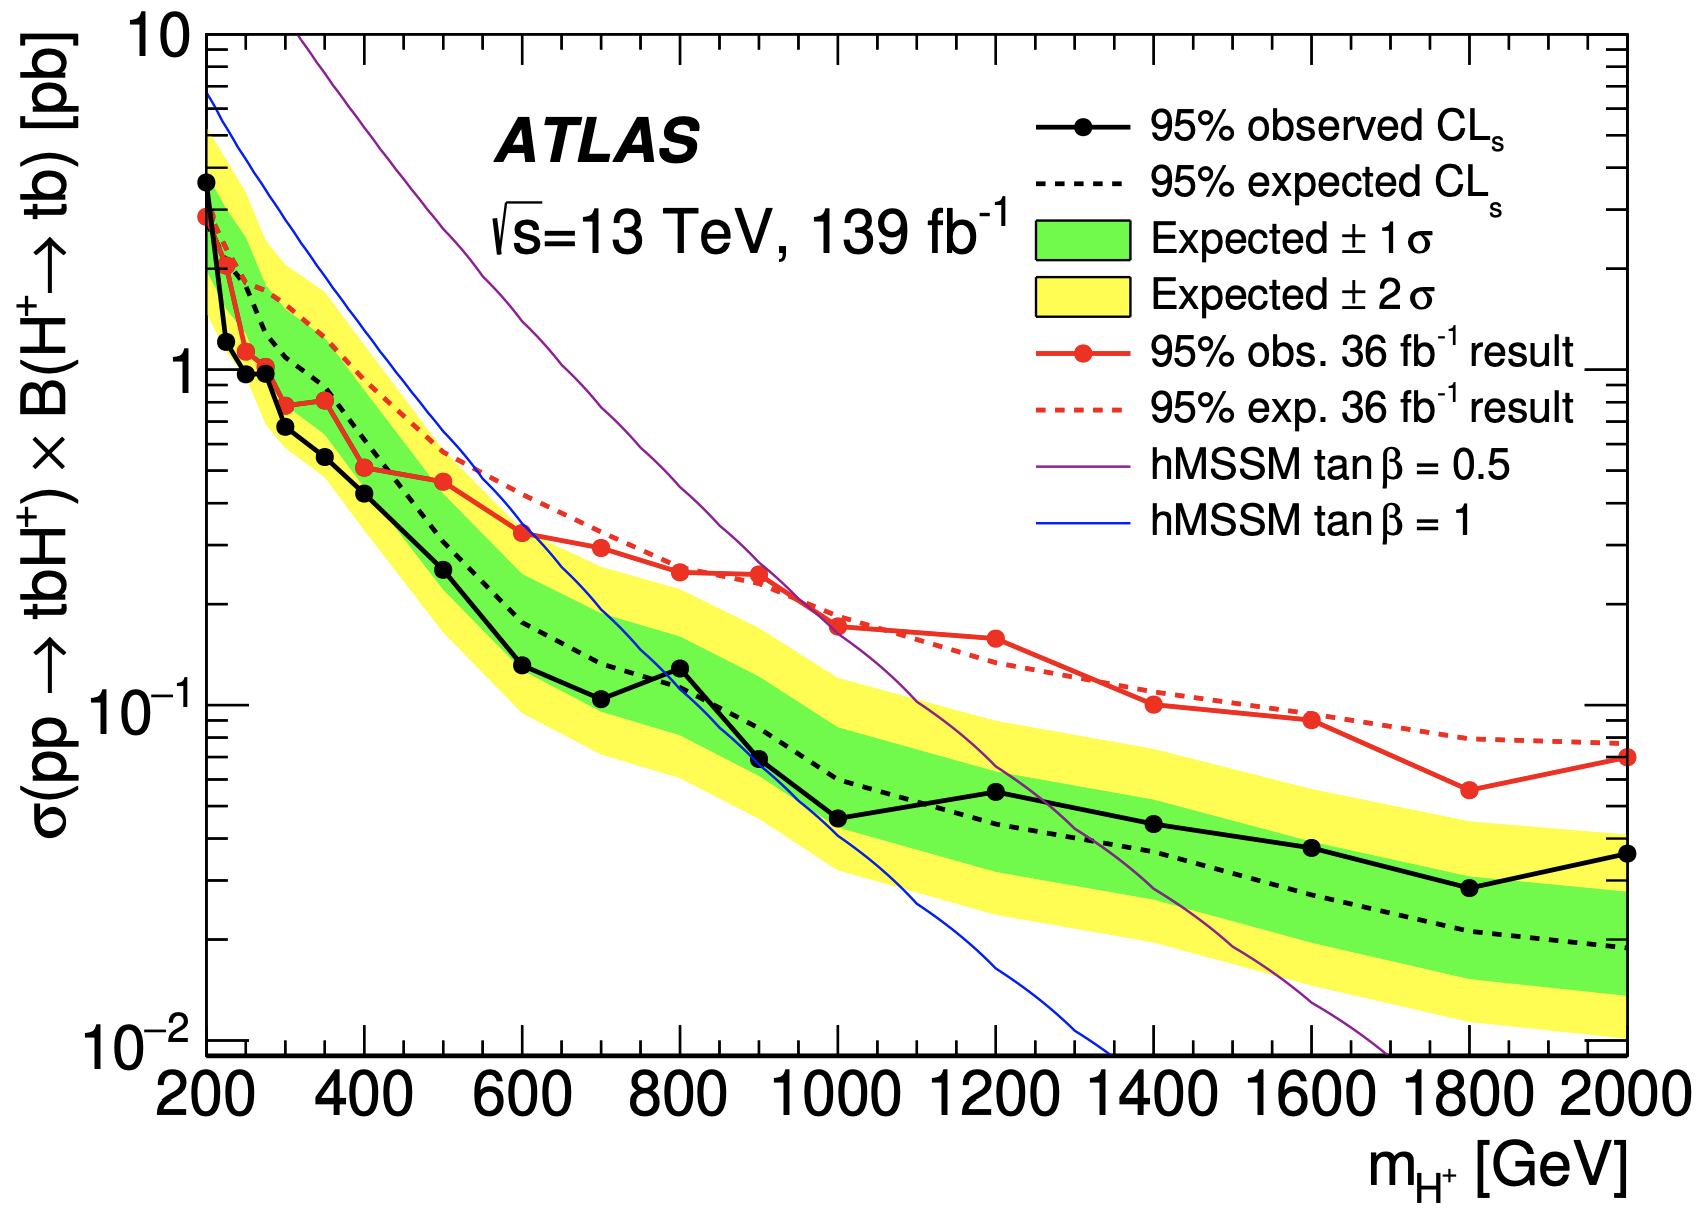
\includegraphics[width=0.75\textwidth]{chapters/chapter2_theory/images/HPlus_to_tb_Limits.png}
			\caption{\label{fig:hpm-tb-limits} Exclusion limits at 95\% CL on $\sigma (pp \to tb\Hpm) \times B(\Hpm \to tb)$ as a function of \mHpm \cite{Hpm-to-tb}. }
		\end{figure}

		\begin{figure}[!ht]
			\centering
			\subfloat[\label{fig:hpm-tb-tanb-limits_a}]{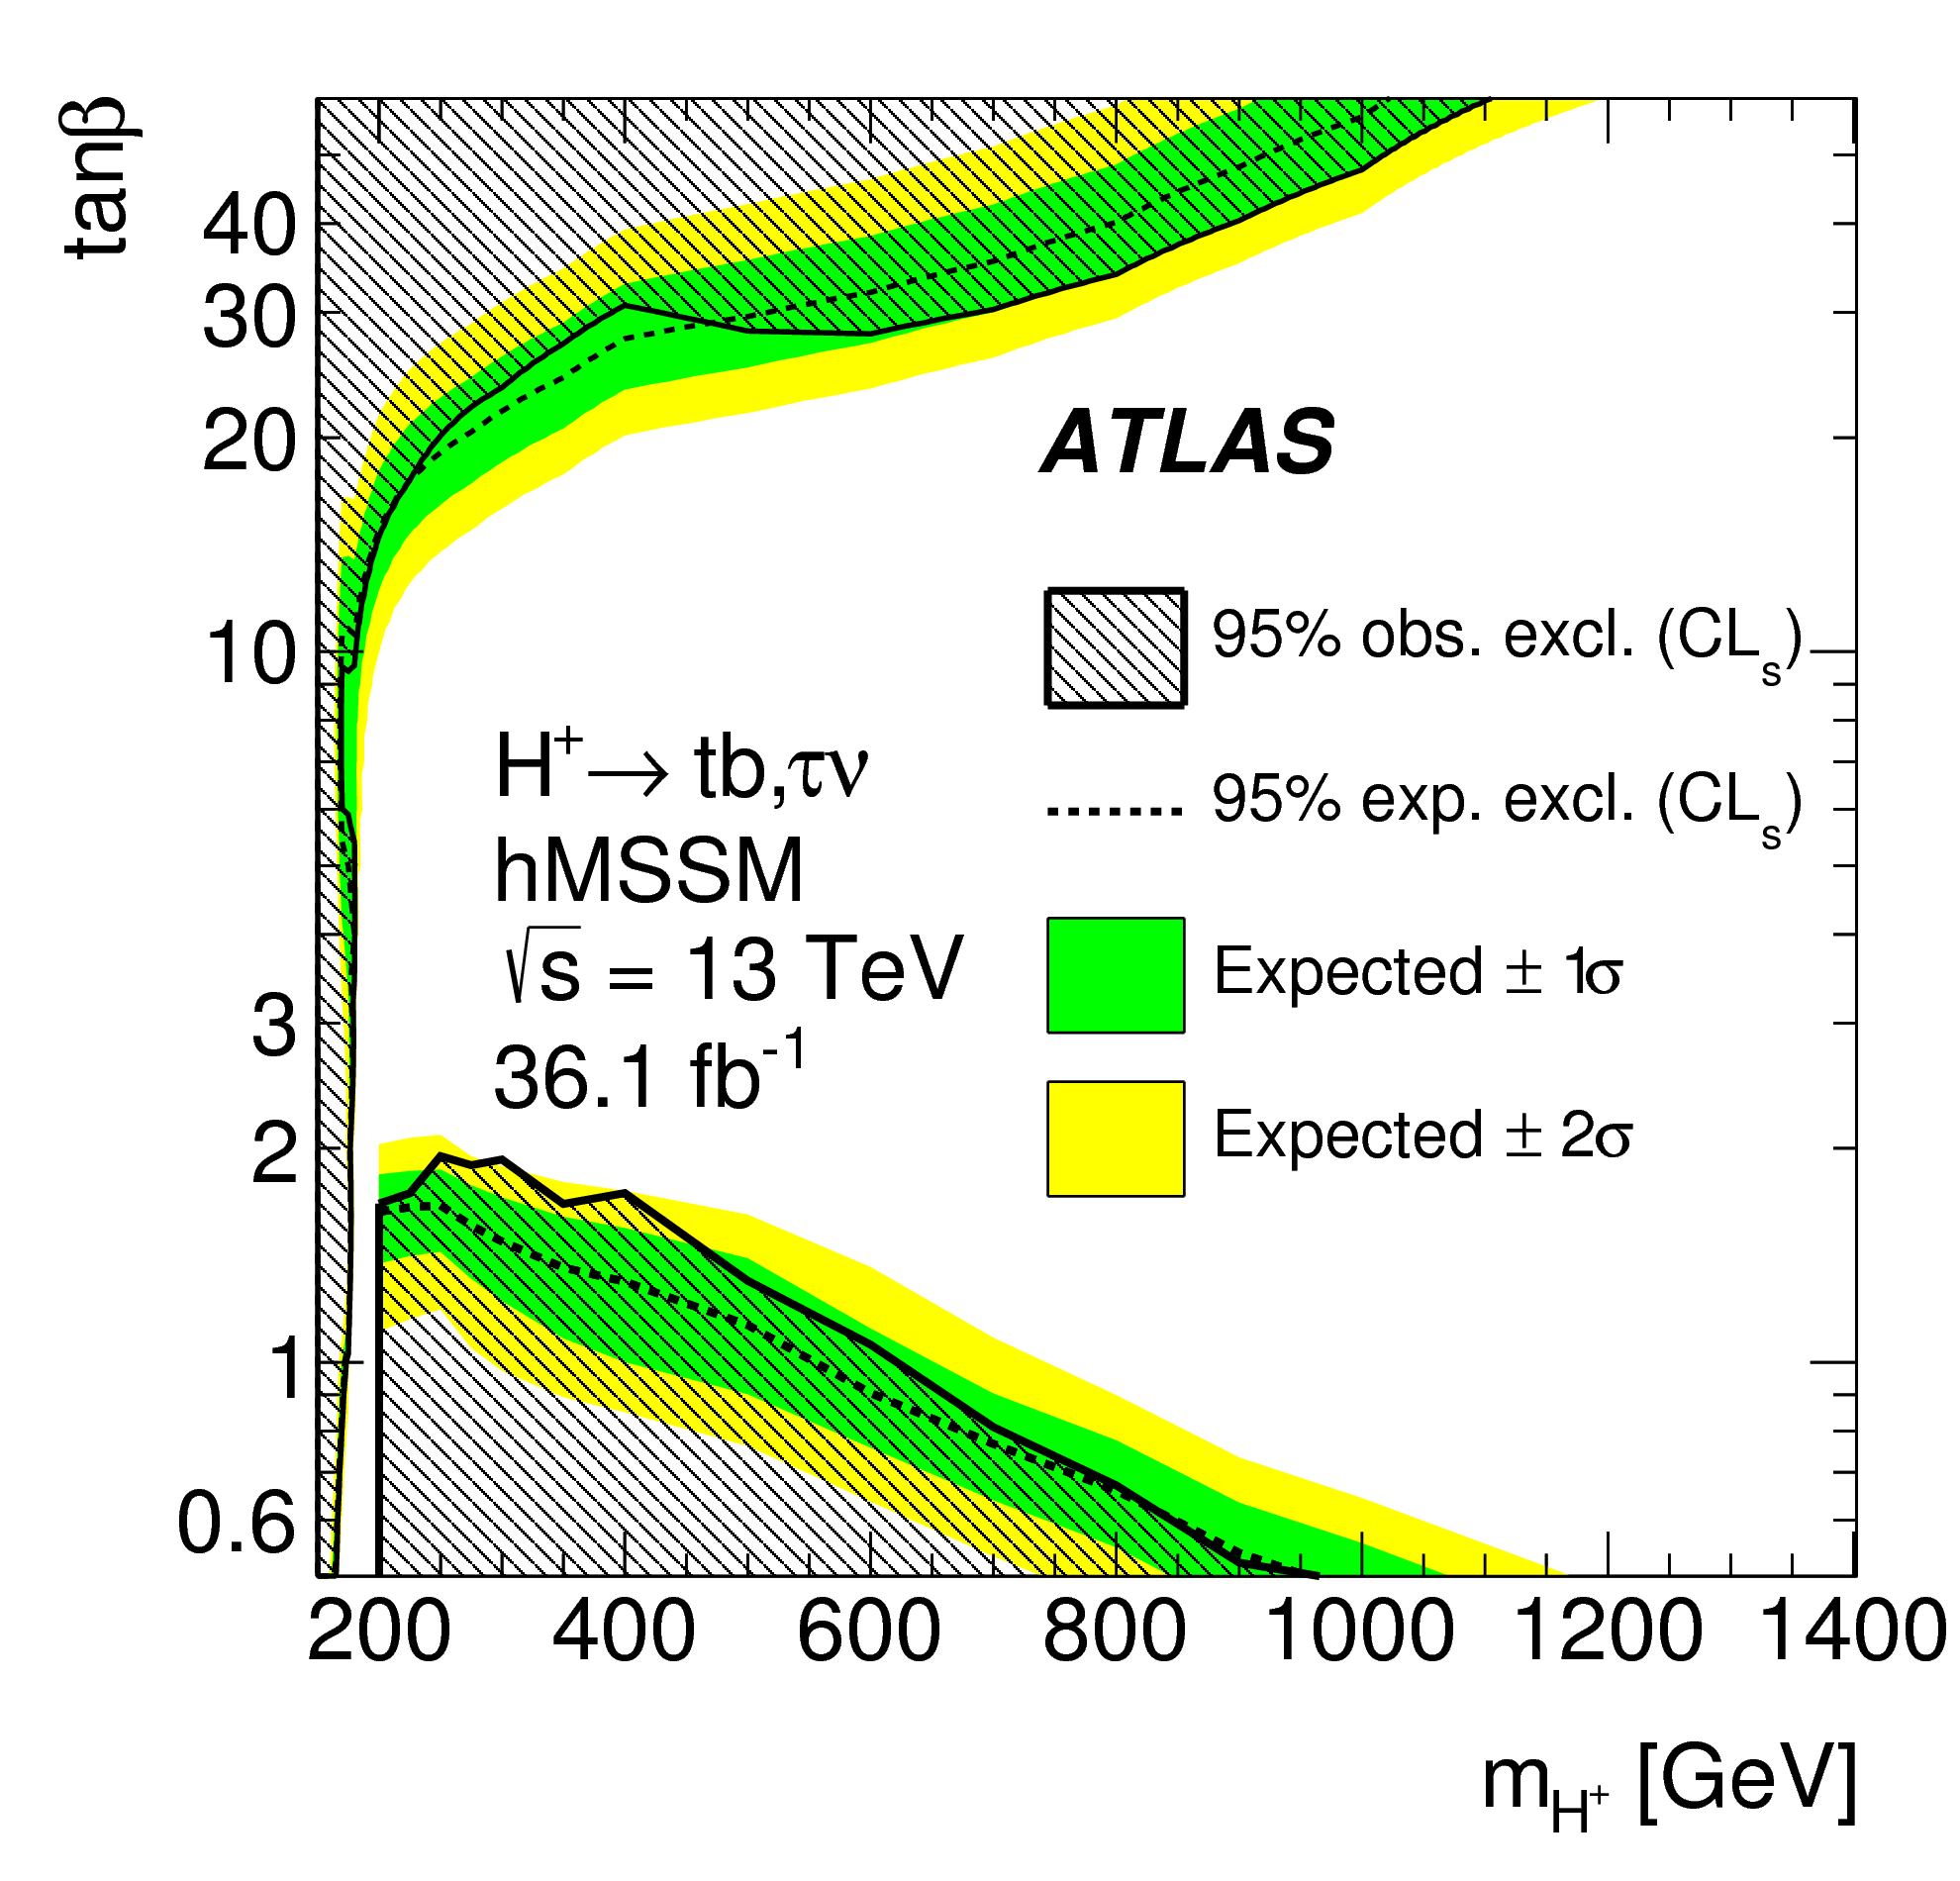
\includegraphics[width=0.5\textwidth,keepaspectratio=true]{defense/HPlus_taunu_tb_tanb_Limits_hMSSM.png}}
			\subfloat[\label{fig:hpm-tb-tanb-limits_b}]{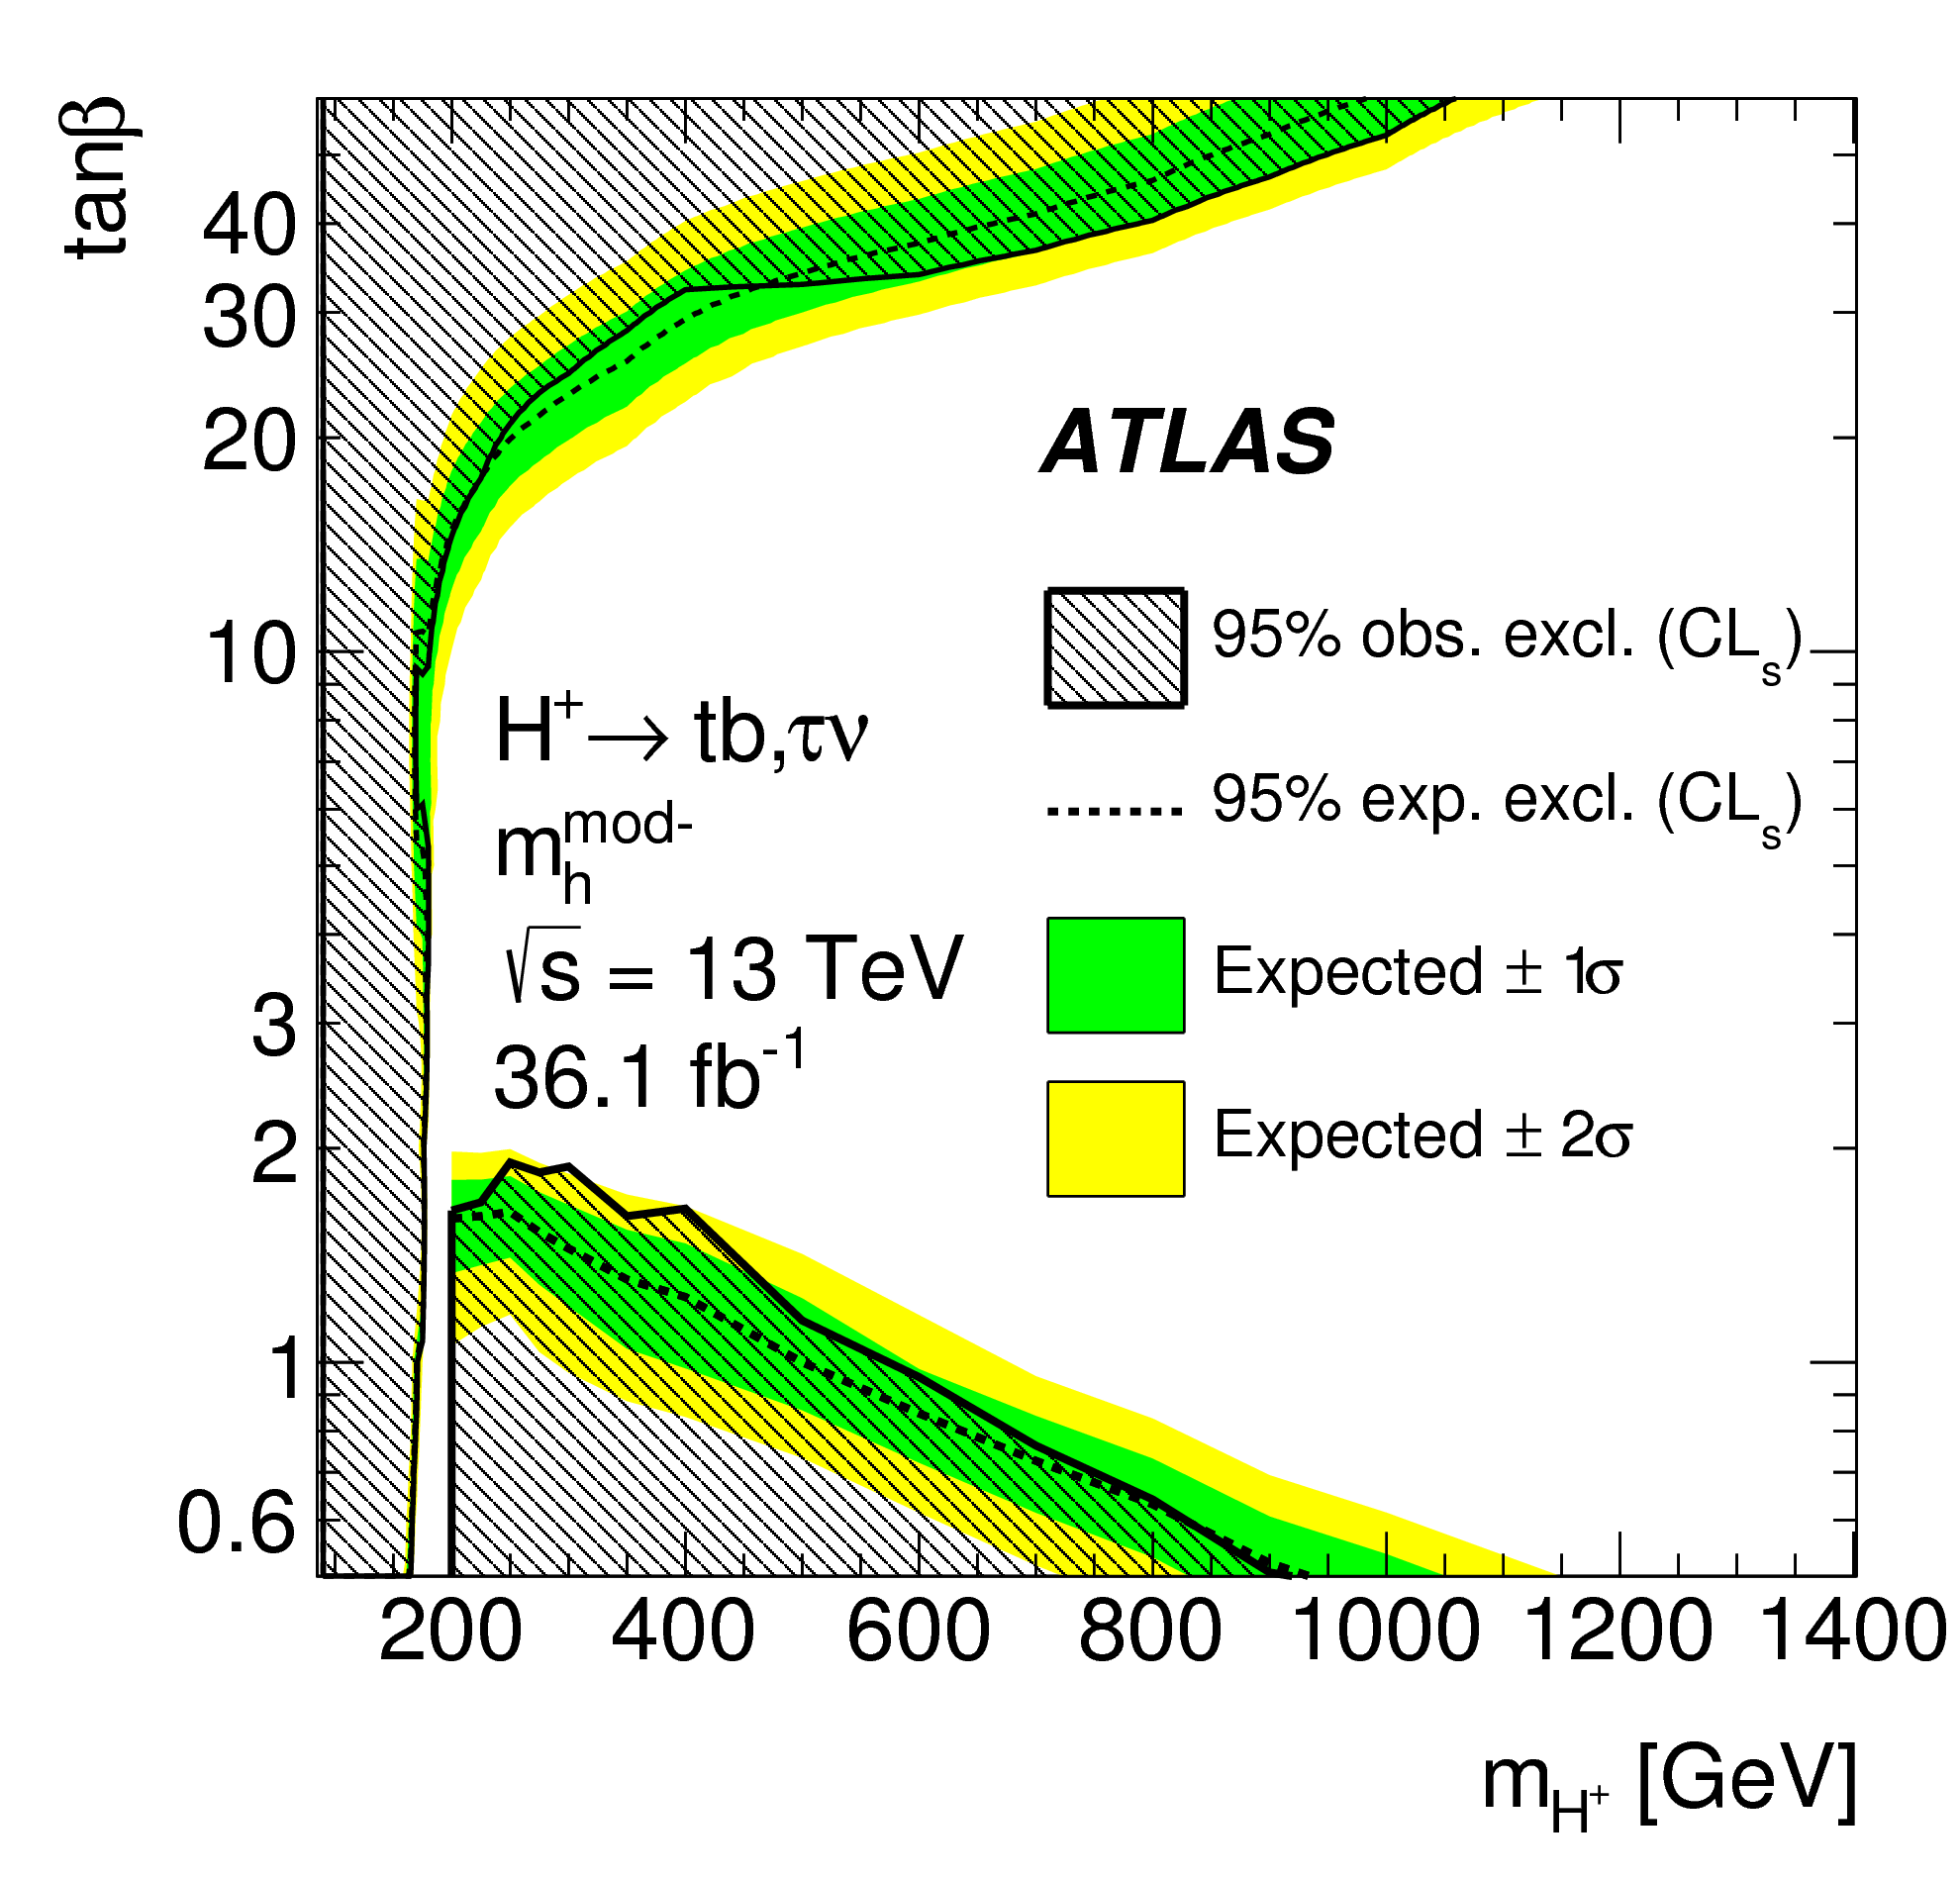
\includegraphics[width=0.5\textwidth,keepaspectratio=true]{defense/HPlus_taunu_tb_tanb_Limits_hMod.png}}
			\caption{\label{fig:hpm-tb-tanb-limits} Exclusion limits at 95\% CL on \tanb as a function of \mHpm in the (a) \gls{MSSM} and (b) $m^{mod+}_{h}$ scenario of the \gls{MSSM} \cite{Hpm-to-tb}. }
		\end{figure}


		The previous iteration of this analysis relied on boosted decision trees (BDT) binned in \mHpm, using five separate classifiers to cover the mass range of $90 - 2000$ GeV. The mass bins can be seen as the blue dotted lines in Figure \ref{fig:hpm-prev-limits_c}. It is important to note the inclusion of the mass range $90 - 200$ GeV, as Reference \cite{hpm-previous} was the first search to include this mass region below the top quark mass.
\chapter{Experimental Apparatus}\label{chap:experiment}

\section{Particle Accelerators}\label{sec:accelerators}
	To study the \gls{SM}, the Higgs boson, and hints of new physics, particle accelerators are used. Particle accelerators can be categorized as either fixed target or colliders. As the naming suggests, in a fixed target accelerator the beam hits a target that then produces the desired particle collisions. A collider uses two beams, often in a circle, that are brought to collide inside a detector. The center of mass energy ($E_{CM}$) of a fixed target accelerator energy scales as the square root of the beam energy ($E_{beam}$), $E_{CM} = \sqrt{E_{beam}}$, whereas a collider scales as $E_{CM} = 2 \, E_{beam}$. Colliders are the preferred accelerator for maximizing the center of mass energy. The analyses discussed in this dissertation use a particle collider.

	\subsection{Hadron Colliders}\label{ssec:hadron-colliders}
		Collider beams are typically made of either leptons or hadrons. Lepton colliders are often considered to as precision machines, as the longitudinal momentum is known and backgrounds are clean. The center of mass energy is well controlled in a lepton collider, meaning particles can be produced on resonance, increasing the desired particle yield. On the other hand, due to the nature of hadrons not being fundamental particles a hadron collider produces a wide variety of collisions; making hadron colliders well suited for discovery but also making for messier backgrounds. The constituents of a hadron participate in the collisions, meaning it is impossible to know the exact longitudinal momentum of the initial state, instead momentum in the transverse plane is used (\pt). The synchrotron radiation produced from a hadron collider is typically much lower than that of a lepton collider; meaning the beams are easier to control and can be pushed to higher energies without extra loses. The analyses discussed in this dissertation use a hadron collider, the \acrlong{LHC}.

		% The center of mass energy scales with $\frac{1}{m^4}$ in a hadron collider; leading to an increased energy gain by simply using heavier particles.

	\subsection{The Large Hadron Collider}\label{ssec:LHC}
		The \acrfull{LHC} is a 27 km circumference circular collider built outside of Geneva, Switzerland at \acrfull{CERN}. At center of mass energy $13$ TeV ($6.5$ TeV in each beam), the \gls{LHC} is the largest and highest energy particle accelerator ever built \cite{lhc-machine}. There are four main collision points along the \gls{LHC}: the \gls{ATLAS}, \gls{CMS}, ALICE, and LHCb experiments. \gls{ATLAS} and \gls{CMS} are general purpose particle detectors while ALICE and LHCb focus on heavy ion collisions. The numbers stated in the following sections are in reference to proton-proton collisions.

		The LHC consists of 1104 NbTi superconducting dipole magnets, each being 15 m long, weighing 35 tonnes, cooled to 2 K, operating at 11,000 Amps, and produce a magnetic field of 8.3 T. A cross-section of a dipole magnet and the surrounding cryogenic system can be see in Figure \ref{fig:dipole-xsec}. The dipole magnets are used to bend the beam around the ring with another 128 used in the beam dump system to remove the beam safely from the \gls{LHC}. A 2-in-1 configuration is used within the dipole magnets to create the required magnetic fields to bend two equally charged beams in opposite directions. A diagram of the magnetic fields in this configuration produced can be seen in Figure \ref{fig:dipole-field}. To focus the beam in the horizontal and vertical planes two quadrapole magnets are used; one magnet focuses in one plane while defocusing in the other. The end result is a horizontally and vertically focused beam. While in the \gls{LHC}, the hadrons are accelerated using radiofrequency cavities. Each oppositely circulating beam is not a solid column of protons but instead consists of 2808 bunches of protons with $1.2 \times 10^{11}$ protons per bunch. Collisions occur when bunches are brought to collide in a bunch crossing. Table \ref{tab:LHC} lists some information on the \gls{LHC}. 

		\begin{table}[!thp]
			\centering
			\caption{\gls{LHC} parameters  \cite{lhc-facts}}
			\begin{tabular}{| l | l |}  
			\hline
			Circumference 						& $26,659$ m 					\\ 	\hline
			Dipole operating temperature 		& $1.9$ K 						\\ 	\hline
			Dipole magnets 						& $1232$ 						\\	\hline
			Quadrapole magnets 					& $392$ 						\\	\hline
			Radiofrequency cavities 			& $16$ ($8$ per beam) 			\\ 	\hline
			Beam energy 						& $6.5$ TeV ($13$ CM TeV) 		\\ \hline
			Protons per bunch 					& $1.2 \times 10^{11}$ 			\\ \hline
			Bunches per beam 					& $2808$ 						\\ \hline
			Revolutions per second 				& $11245$ 						\\ \hline
			Collisions per second 				& $1,000,000,000$ 				\\ \hline
			\end{tabular}
			\label{tab:LHC}
		\end{table}

		\begin{figure}[!ht]
		\centering
		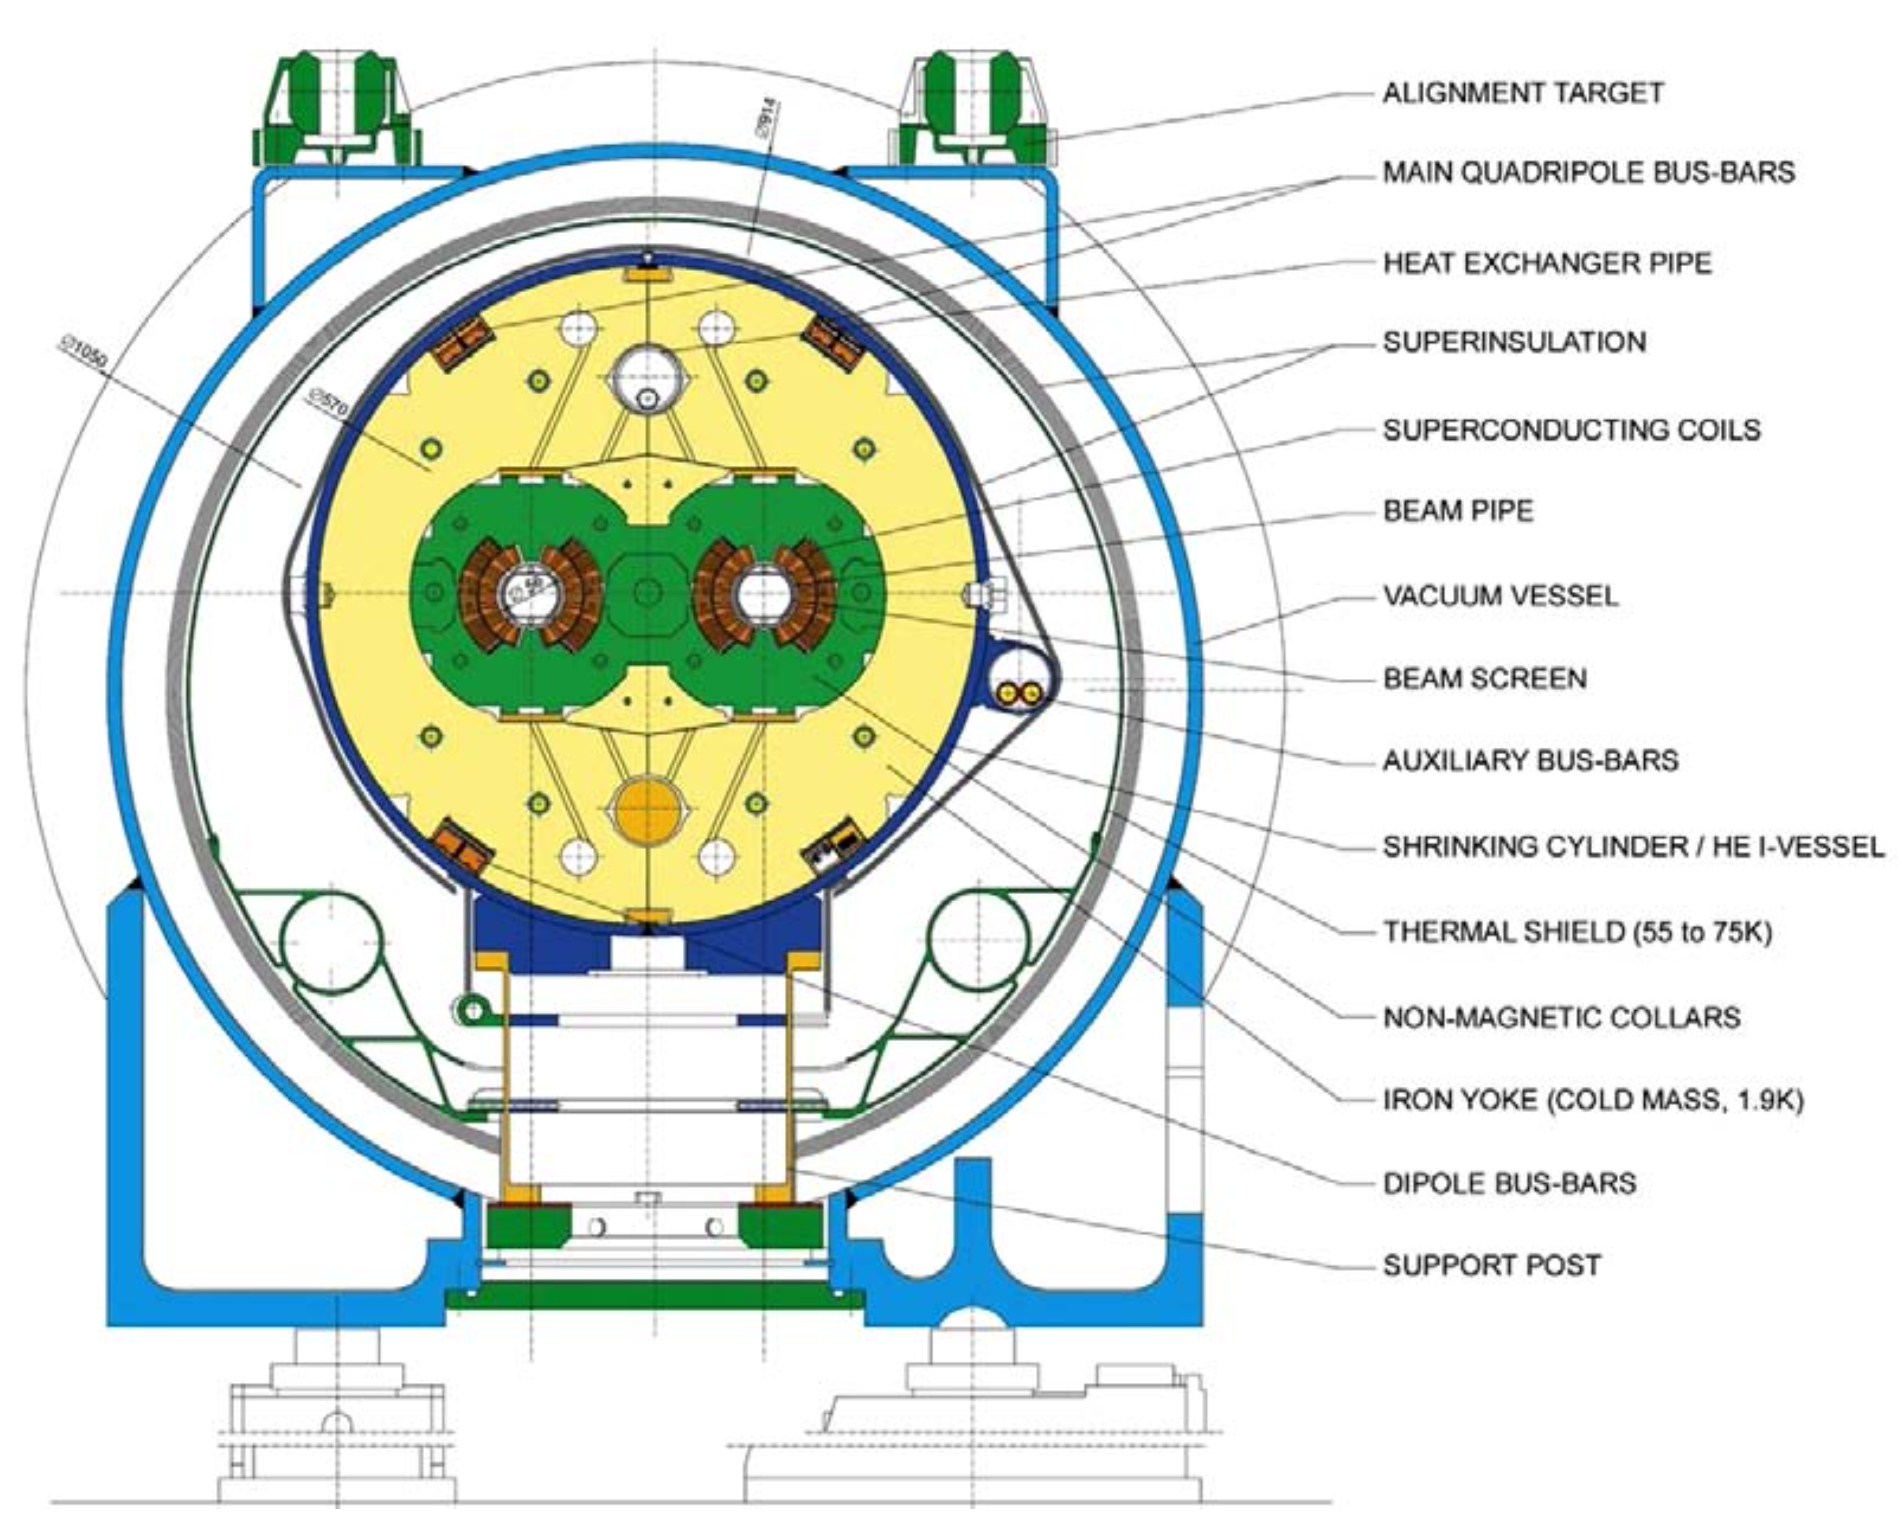
\includegraphics[width=\textwidth,keepaspectratio=true]{chapters/chapter3_experiment/images/dipole-crosssection.png}
		\caption{Cross-section of cryodipole (lengths in mm). \cite{lhc-machine}}
		\label{fig:dipole-xsec}
		\end{figure}

		\begin{figure}[!ht]
		\centering
		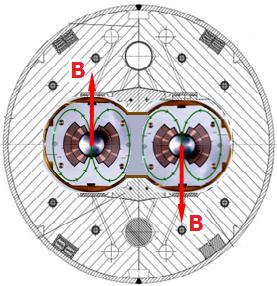
\includegraphics[width=.45\textwidth,keepaspectratio=true]{chapters/chapter3_experiment/images/dipole-field.jpeg}
		\caption{Field of the \gls{LHC} dipole magnets. \cite{dipole-field}}
		\label{fig:dipole-field}
		\end{figure}

	\subsection{CERN Accelerator Complex}\label{ssec:cern-accelerators}
		There are a series of accelerators used to get each beam up to its final energy of 6.5 TeV. The protons used in collisions are sourced from hydrogen atoms. The hydrogen is ionized, leaving the nucleus consisting of one proton, these protons are then accelerated in radiofrequency (RF) cavities. Figure \ref{fig:CERN-complex} shows in detail the full accelerator complex at CERN.\footnote{Figure \ref{fig:CERN-complex} shows the newer LINAC 4 at the start of Run-3. This work is concerning data taken with LINAC 2.} 
		\begin{figure}[!ht]
		\centering
		\includegraphics[width=\textwidth,keepaspectratio=true]{chapters/chapter3_experiment/images/CERN-complex.png}
		\caption{The CERN accelerator complex. \cite{CERN-complex}}
		\label{fig:CERN-complex}
		\end{figure}
		The protons used in the \gls{LHC} start the accelerating process in the linear accelerator LINAC 2. They then are accelerated in the booster, PS, SPS, and are finally injected at the \gls{LHC} where they are accelerated to the final 6.5 TeV beam energy. The final energies of protons from each accelerator can be seen in Table \ref{tab:accelerator-complex}.
		\begin{table}[!thp]
			\centering
			\caption{Accelerator final energies}
			\begin{tabular}{| l | l |}  
			\hline
			Accelerator 					& Final Energy 	\\ \hline
			\hline
			LINAC 2 						& $50$ MeV 		\\ 	\hline
			Booster 						& $1.4$ GeV 	\\ 	\hline
			Proton Synchrotron (PS)			& $26$ GeV 		\\ 	\hline
			Super Proton Synchrotron (SPS) 	& $450$ GeV 	\\ 	\hline
			Large Hadron Collider (LHC)		& $6.5$ TeV 	\\ 	\hline
			\end{tabular}
			\label{tab:accelerator-complex}
		\end{table}
		Once the beams are at final collision energy they are then focused, aligned, and squeezed using the series of magnets discussed above. The term stable beams is used to refer to the status of the beams within the LHC when they have reached optimal conditions for data taking.

	\subsection{Luminosity}\label{ssec:lumi}
		The amount of data collected from colliders is often referred to in terms of luminosity. Luminosity is measured in terms of inverse barns, where $1 \, b = 10^{-28} \, m^2$. The instantaneous luminosity of one bunch crossing can be written as 
		\begin{equation}\label{eqn:bunch-lumi}
		\mathcal{L}_{bunch} = \frac{ \mu  f }{\sigma}
		\end{equation}
		where $\sigma$ is the cross section and can be thought of as the probability of a collision occurring, $\mu$ is the number of inelastic interactions per bunch crossing, and $f$ is the revolution frequency of the LHC $f=11246$ Hz. Therefore, the total instantaneous luminosity is 
		\begin{equation}\label{eqn:tot-inst-lumi}
		\mathcal{L} = N_b \frac{ \langle \mu \rangle f}{\sigma}
		\end{equation}
		where $\langle \mu \rangle$ is the average number of inelastic interactions per bunch crossing. 

		The integrated luminosity then corresponds to the total amount of data that was taken during a time period and can be seen for the LHC Run-2 in \ref{fig:lhc-lumi}
		\begin{figure}[!ht]
		\centering
		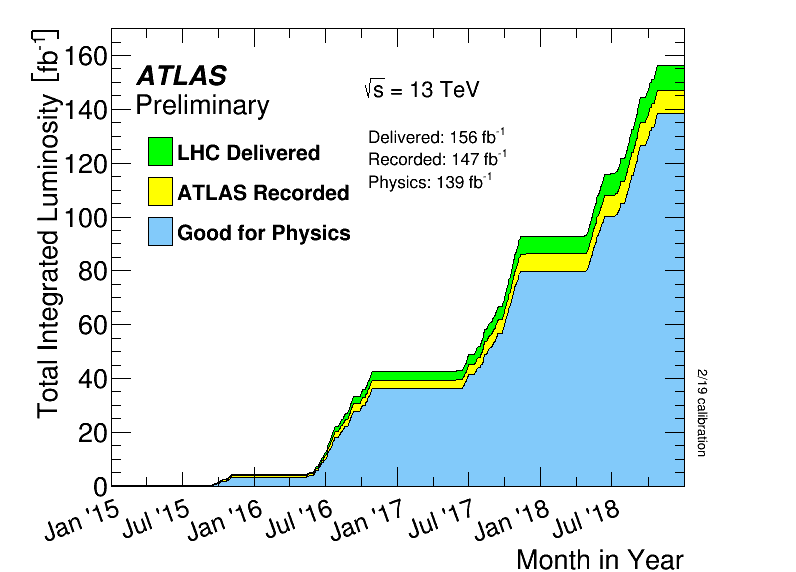
\includegraphics[width=.65\textwidth,keepaspectratio=true]{chapters/chapter3_experiment/images/intlumivstimeRun2DQall.png}
		\caption{ Cumulative luminosity versus time delivered to \gls{ATLAS} (green), recorded by \gls{ATLAS} (yellow), and certified to be good quality data (blue) during stable beams for pp collisions at 13 TeV center of mass energy in 2015-2018. The difference between the colored histograms reflects inefficiencies, especially those seen when restarting data taking \cite{luminositypublicresultsrun2}.}
		\label{fig:lhc-lumi}
		\end{figure}
		The value of $\langle \mu \rangle$ changed throughout data taking and can be seen in Figure \ref{fig:run2-mu} and is referred to as pileup because the higher the $\langle \mu \rangle$ value, the more messy a collision becomes.
		\begin{figure}[!ht]
		\centering
		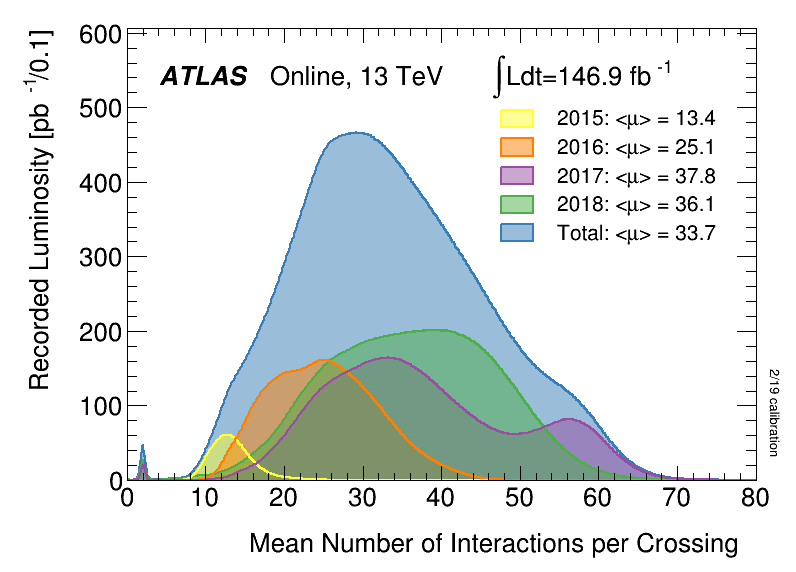
\includegraphics[width=.65\textwidth,keepaspectratio=true]{chapters/chapter3_experiment/images/mu_2015_2018.png}
		\caption{ The luminosity-weighted distribution of the mean number of interactions per bunch crossing for the 2015-2018 \pp collision dataset at $13$ TeV center of mass energy \cite{luminositypublicresultsrun2}.}
		\label{fig:run2-mu}
		\end{figure}
		The effect of high pileup can be seen in Figure \ref{fig:high-pileup-event-display}, a collision event taken in 2018 with 29 reconstructed vertices shown on the bottom right as colored circles.
		\begin{figure}[!ht]
		\centering
		\includegraphics[width=\textwidth,keepaspectratio=true]{chapters/chapter3_experiment/images/event_display_r349114_e216445472_v4_wMoreTracks_v3_wAtlantisTrackColor_Inset.png}
		\caption{ A display of a candidate Z boson event from proton-proton collisions recorded by \gls{ATLAS} with \gls{LHC} stable beams at a collision energy of 13 TeV. The Z boson candidate is reconstructed in a beam crossing with 28 additionally reconstructed primary vertices from the minimum bias interactions. The candidate event is reconstructed in the 2$\mu$ final state. In the left display, the red lines show the path of the two muons including the hits in the muon spectrometer and the orange tracks are the remaining charged particles from the 29 vertices, with transverse momentum above 0.5 GeV. The colored squares in the lower display correspond to the position of the reconstructed vertices. The invariant mass of the two muons is 92.3 GeV \cite{eventdisplayrun2physics}. }
		\label{fig:high-pileup-event-display}
		\end{figure}


		A common calculation using the total integrated luminosity is shown in Equation \ref{eqn:tot-proc-num}; where the number of times a particular process was produced is calculated.
		\begin{equation}\label{eqn:tot-proc-num}
		N_{x} = \mathcal{L} \sigma_{x}
		\end{equation}
		where again, $\sigma$ is the cross section. In this case, the cross section corresponding to process $x$.


\section{The \gls{ATLAS} Detector}\label{sec:ATLAS}
	The \acrfull{ATLAS} detector is one of two general purpose particle detectors on the \gls{LHC}; the other being the \acrfull{CMS}. \gls{ATLAS} is comprised of four main components: the inner detector, calorimeters, muon system, and the magnet system. Each component has several types of technology in order to measure the energy, trajectories, and determine the original particle of all possible particle decays.\footnote{Neutrinos are not directly detected, but inferred via a missing transverse energy calculation described in Section \ref{sec:reco-etmiss}.} The full \gls{ATLAS} detector measures 44 m in length, 25 m in diameter, and weighs over 7000 tonnes \cite{ATLAS-JINST} . Figure \ref{fig:ATLAS} shows a 3D model of the \gls{ATLAS} detector.\footnote{Figure \ref{fig:ATLAS} shows the New Small Wheel muon-chambers. This dissertation concerns data collected with the old Small Wheel muon-chambers.} All of the subdetectors output data to the \gls{TDAQ} system that selects collisions with interesting physics using a complex mix of hardware and software algorithms detailed in Section \ref{ssec:trigger}. 

	\begin{figure}[!ht]
	\centering
	% 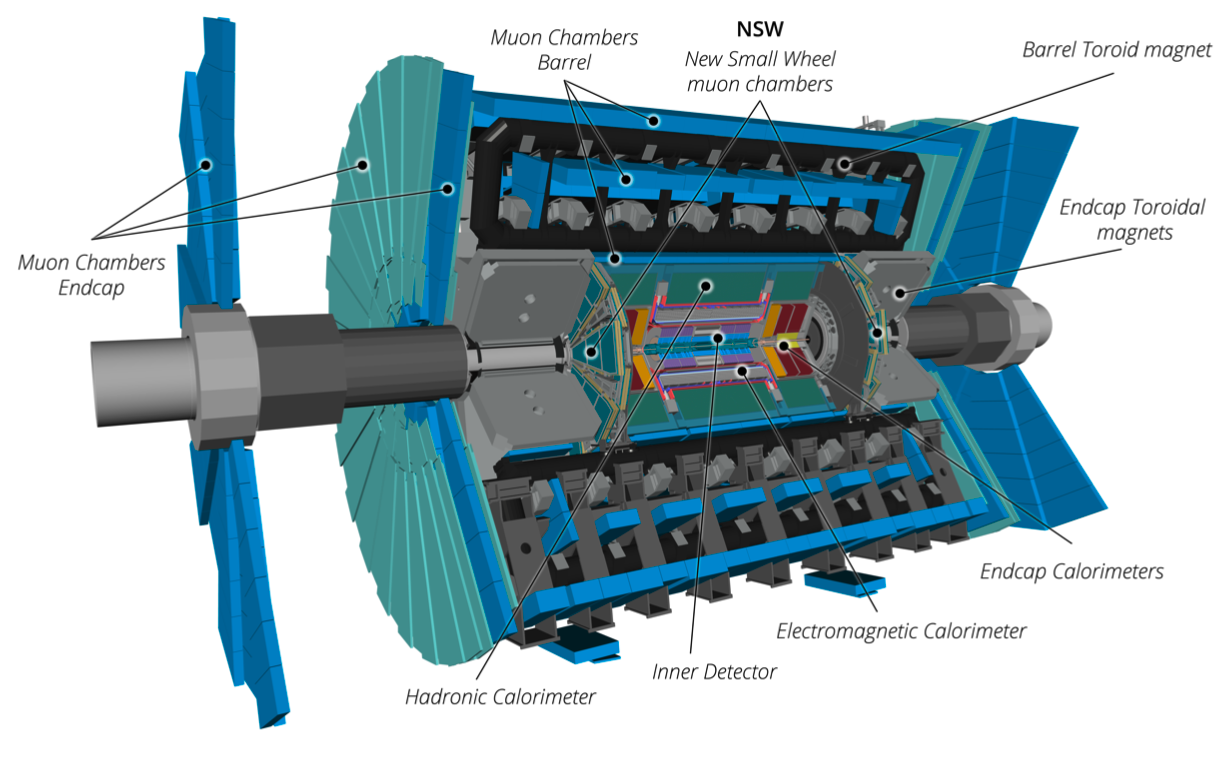
\includegraphics[width=.75\textwidth,keepaspectratio=true]{chapters/chapter3_experiment/images/ATLAS_3d_run3.png}
	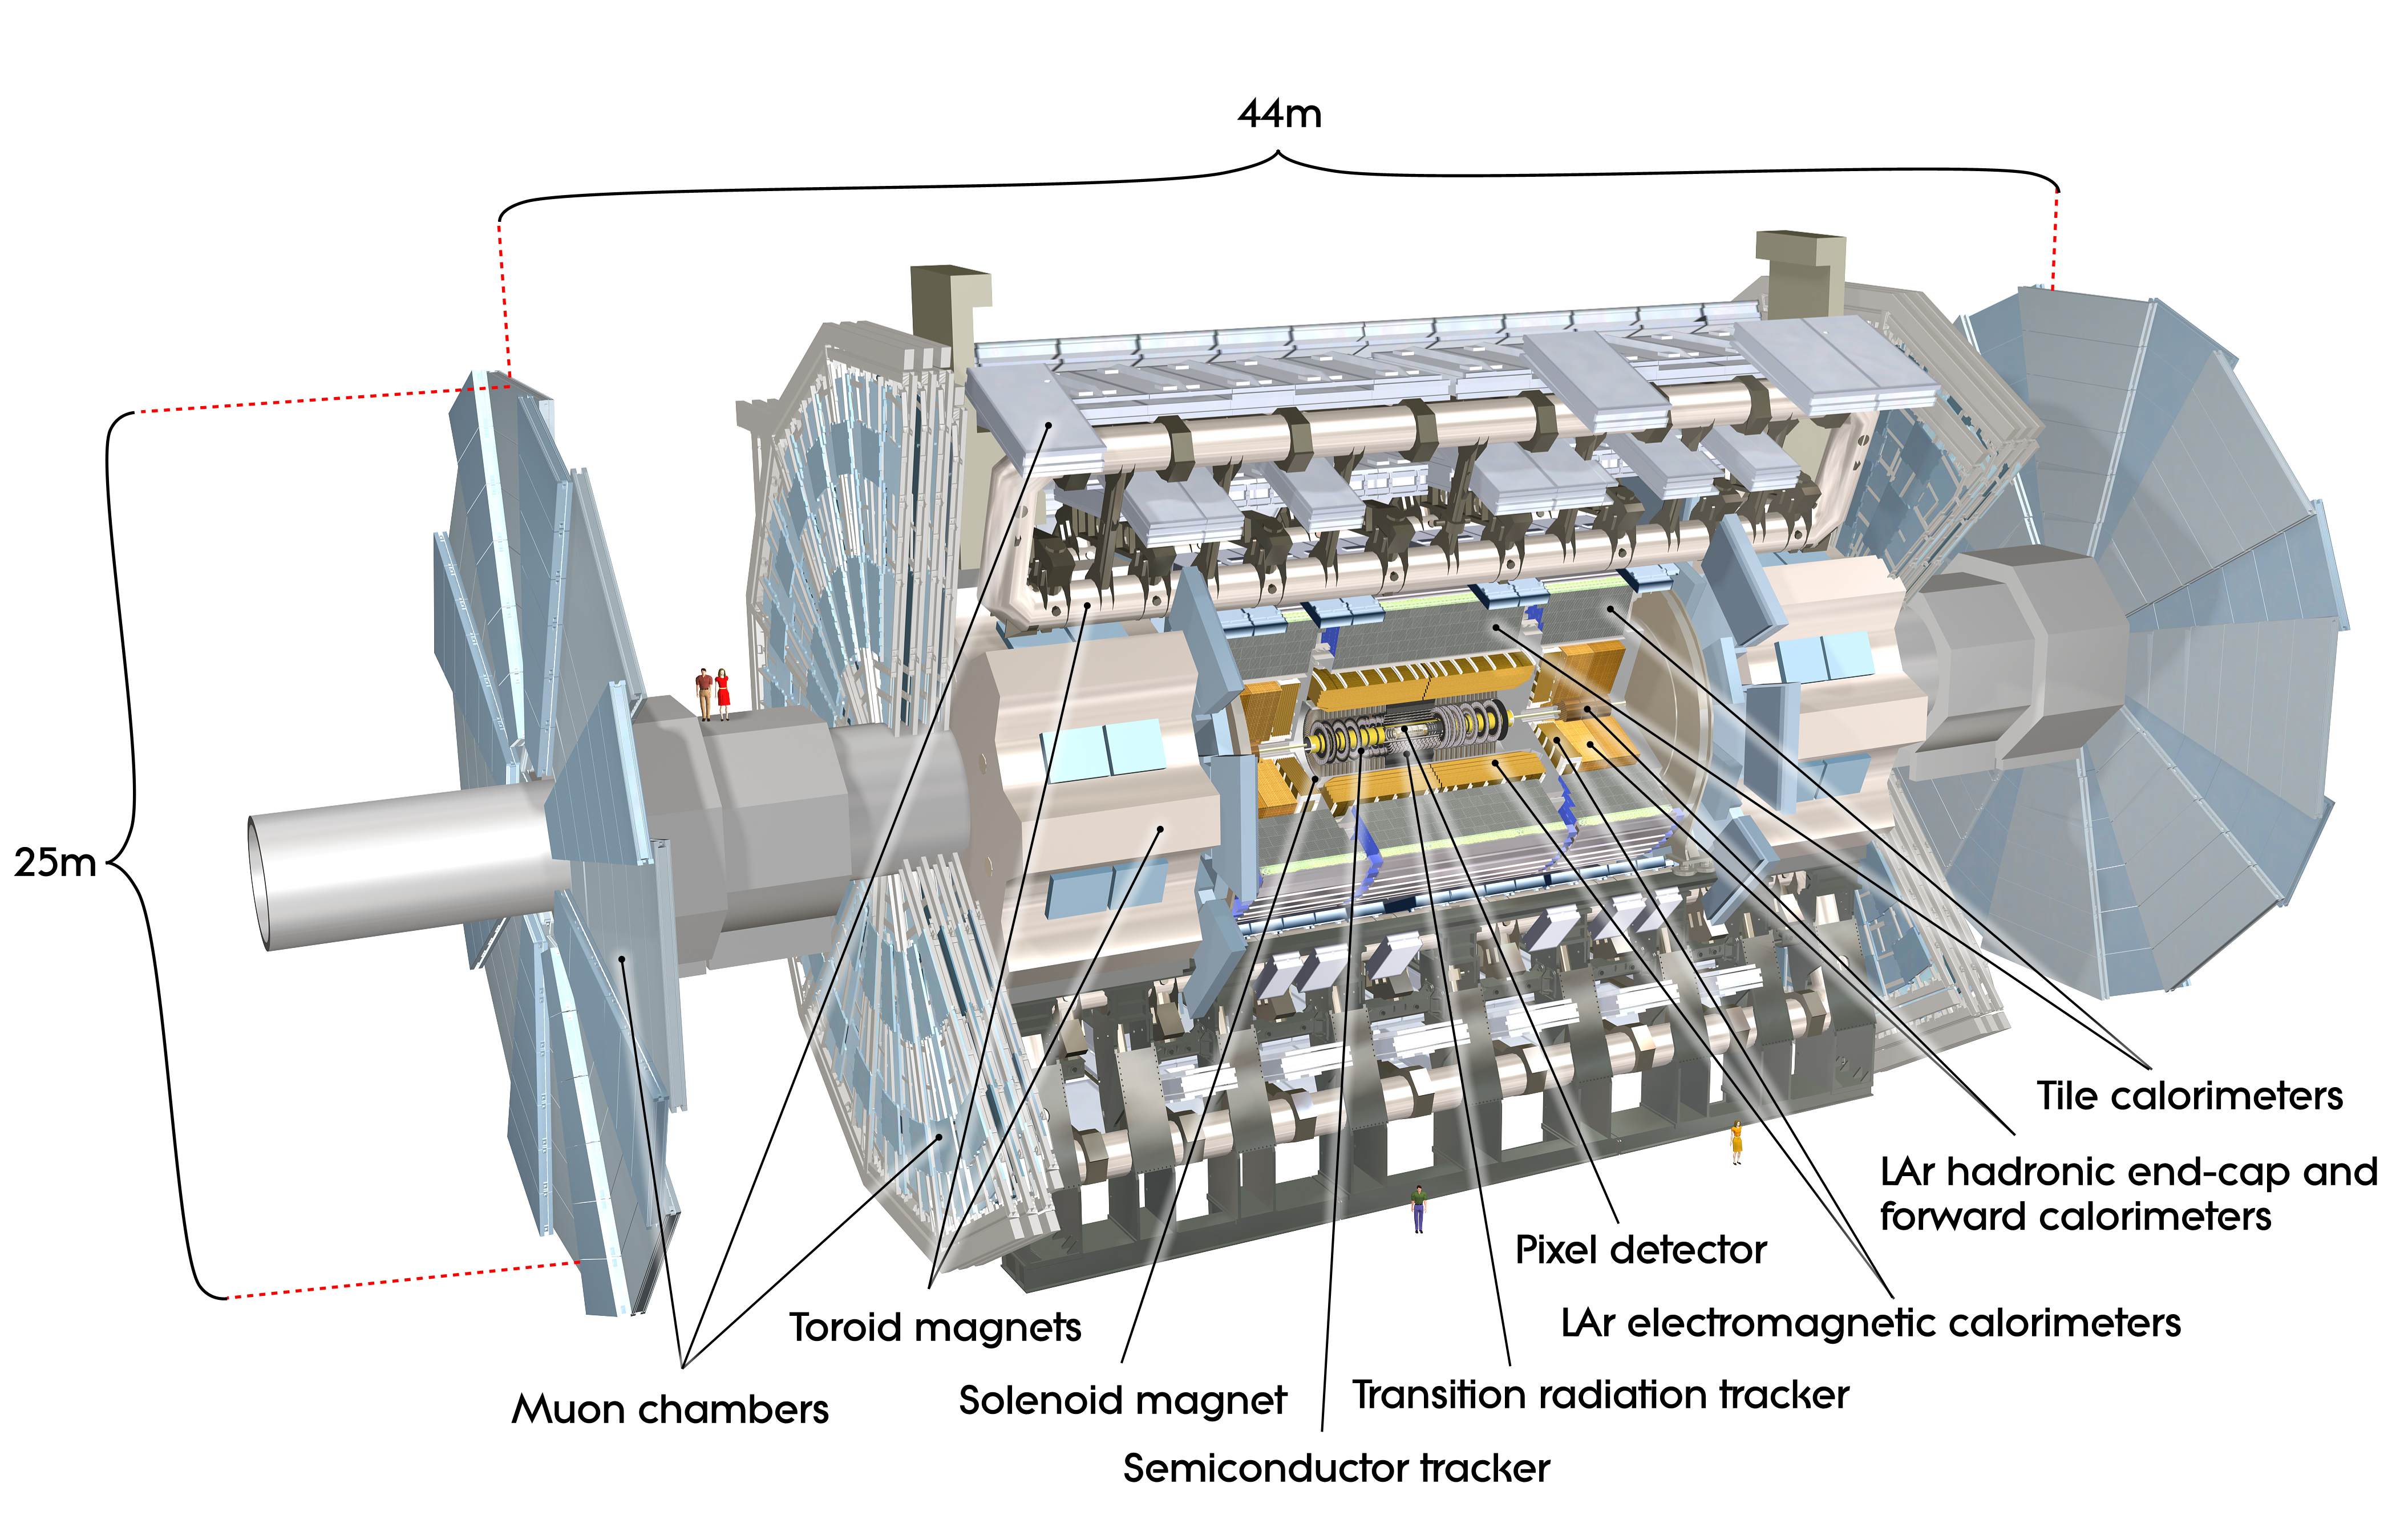
\includegraphics[width=.75\textwidth,keepaspectratio=true]{chapters/chapter3_experiment/images/ATLAS_3d_run2.jpg}
	\caption{ Cut-away view of the \gls{ATLAS} detector with major subdetectors highlighted. \cite{atlas-schematics}}
	\label{fig:ATLAS}
	\end{figure}


	% and Figure \ref{fig:ATLAS-XSec} shows a cross section of the detector and various particles trajectory.
	% \begin{figure}[!ht]
	% \centering
	% 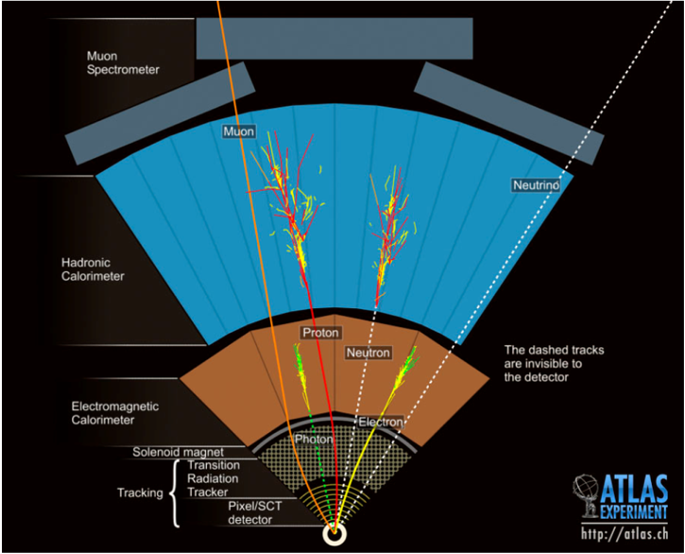
\includegraphics[width=.65\textwidth,keepaspectratio=true]{chapters/chapter3_experiment/images/ATLASCrossSectionDiagram.png}
	% \caption{ Cross section view of the ATLAS detector with subdetectors labeled. Various types of particles radial trajectories are shown.}
	% \label{fig:ATLAS-XSec}
	% \end{figure}

	\subsection{Detector Coordinates}\label{ssec:coordinates}
		Since \gls{ATLAS} is a cylinder\footnote{The \gls{ATLAS} detector is not a perfect cylinder but can be closely approximated as one.}, it is convenient to start with polar cylindrical coordinates. For \gls{ATLAS}, the z-axis is in line with the beam line, the x-axis points towards the center of the \gls{LHC} ring, and the y-axis points vertically. However, since particle collisions are relativistic by nature, a set of Lorentz invariant coordinates is much more useful. The radial coordinate $r$ defines the radial distance from the \gls{IP} at the center of \gls{ATLAS}, $\phi$ is the azimuthal angle describing the angle from the x axis and $\eta$, the pseudorapidity, is defined as 
		\begin{equation}\label{eqn:eta}
		\eta \equiv - \mathrm{ln} \left( \mathrm{tan} \left( \frac{\theta}{2} \right) \right)
		\end{equation}
		where $\theta$ is the angle from the y-axis. The differences in $\eta$ between particles is Lorentz invariant in the coordinate system of $(r,\phi,\eta)$. Due to the large collision energies of the \gls{LHC}, the pseudorapidity is a close estimate to the true rapidity ($y$)\footnote{In this sense, y is now the rapidity, not the y-axis coordinate.} of the particles. 
		\begin{equation}\label{eqn:rapidity}
		y \equiv \frac{1}{2} ln(\frac{E+p_Z}{E-p_Z}) \approx \eta
		\end{equation}
		$\Delta R$ is used to define the distance between two particles.
		\begin{equation}\label{eqn:dR}
		\Delta R \equiv \sqrt{ (\Delta \eta)^2 + (\Delta \phi)^2}
		\end{equation}

		% In the ATLAS detector, the central barrel section corresponds to $|\eta| < 2.5$
		Figure \ref{fig:pseudorapidity} shows visually how $\eta$ relates to $\theta$. In the \gls{ATLAS} detector, the central barrel section generally corresponds to a range of $|\eta|<1$.\footnote{The exact $\abs{\eta}$ range differs between each subdetector.} 

		\begin{figure}[!ht]
		\centering
		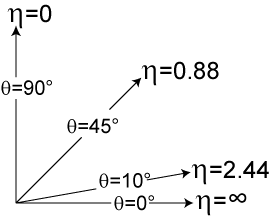
\includegraphics[width=.25\textwidth,keepaspectratio=true]{chapters/chapter3_experiment/images/Pseudorapidity.png}
		\caption{ A diagram showing the pseudorapidity $\eta$ and corresponding $\theta$ values. \cite{pseudorapidity} }
		\label{fig:pseudorapidity}
		\end{figure}

	\subsection{Magnet Systems}\label{ssec:magnets}
	The \gls{ATLAS} detector makes use of two superconducting magnet systems; a central solenoid and a toroid system. Both systems provide large magnetic fields to curve charged particles. The curvature can be used to measure the electromagnetic charge and charge to mass ratio, effectively measuring the momentum of charged particles. Figure \ref{fig:ATLAS-magnets} shows the magnets in \gls{ATLAS}.

	\begin{figure}[!ht]
	\centering
	% 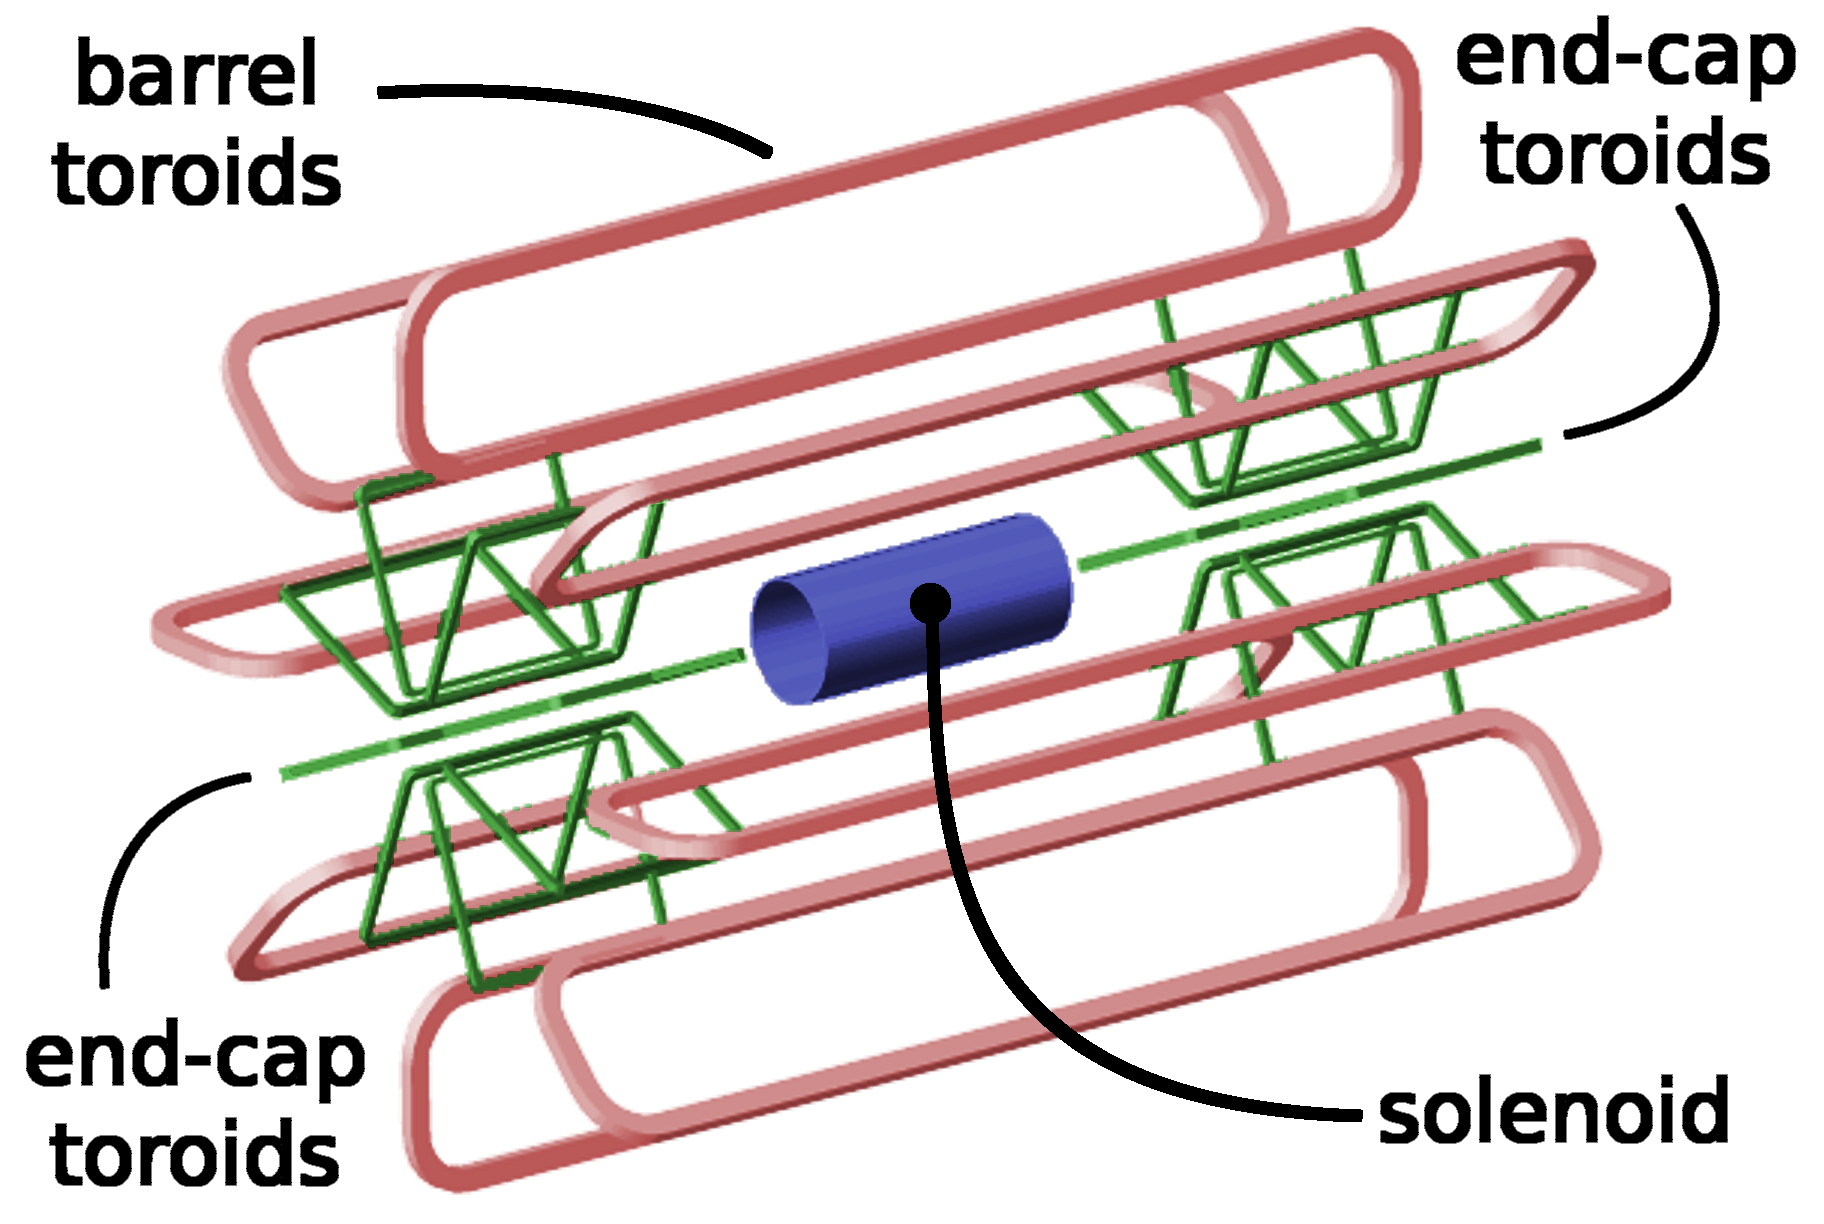
\includegraphics[width=.65\textwidth,keepaspectratio=true]{chapters/chapter3_experiment/images/magnetSystems.png}
	\includegraphics[width=.65\textwidth,keepaspectratio=true]{chapters/chapter3_experiment/images/magnetSystems_3d.png}
	\caption{ The ATLAS magnet systems. \cite{atlas-schematics}}
	\label{fig:ATLAS-magnets}
	\end{figure}

	\subsubsection{Solenoid System}\label{sssec:solenoid}
		The central solenoid encases the \gls{ID}, creating an axially symmetric 2 T magnetic field. This magnetic field bends charged particles in the transverse plane throughout the \gls{ID}. The solenoid magnet itself measures 5.3 m in length and 2.63 m in diameter. In an effort to decrease the amount of material in front of the calorimeters the solenoid magnet was made to be thin. It is a single-layer coil with approximately 1200 turns of NbTi superconducting wires encased in Al-Cu to structurally stabilize the magnet material \cite{atlas-solenoid}. The steel structure within the Tile calorimeter acts as the magnetic flux return for the solenoid magnet system. 70\% of this flux passes through the supporting girder structure, 25\% through the active calorimeter material, and roughly 2\% through the front-plates of the Tile calorimeter \cite{ATLAS-tile}.

	\subsubsection{Toroid System}\label{sssec:toroid}
		The \gls{ATLAS} detector gets its name from the toroidal magnetic system that is critical in the measurements of muon properties. The toroid system bends any charged particles that make it past the calorimeters along the beam axis. This is achieved through a radially symmetric magnetic field of 3.9 T in the barrel and 4.1 in the end-caps. The barrel toroid system is comprised of 8 air core superconducting toroid magnets that each measure 25 m in length, 10 m in diameter, and weigh 750 tonnes. The superconducting wires are the same used in the solenoid, NbTi encased in Al-Cu \cite{atlas-toroid}. Each magnet is encased in a stainless steel cryogenic chamber, or cryostat. The toroid magnet system has two end-cap toroids that are very similar in construction to the barrel toroids. The end-cap toroids also have 8 coils measuring 5 m in length and 10 m in diameter. Instead of individual cryostats for each coil, the end-caps are encased in large cryostats that hold all 8 coils. This allows the end-caps to be pulled out and offers easy access to the rest of the detector. Just like with the central solenoid system, the design of the toroid system was chosen to limit the amount of material between detector components. A solenoid magnet of similar size to the toroid system would not only add more material, but would be cost prohibitive as well.


	\subsection{Inner Detector}\label{ssec:ID}
		\begin{figure}[!ht]
		\centering
		% \subfloat[\label{fig:hpm-diagrams_a}]{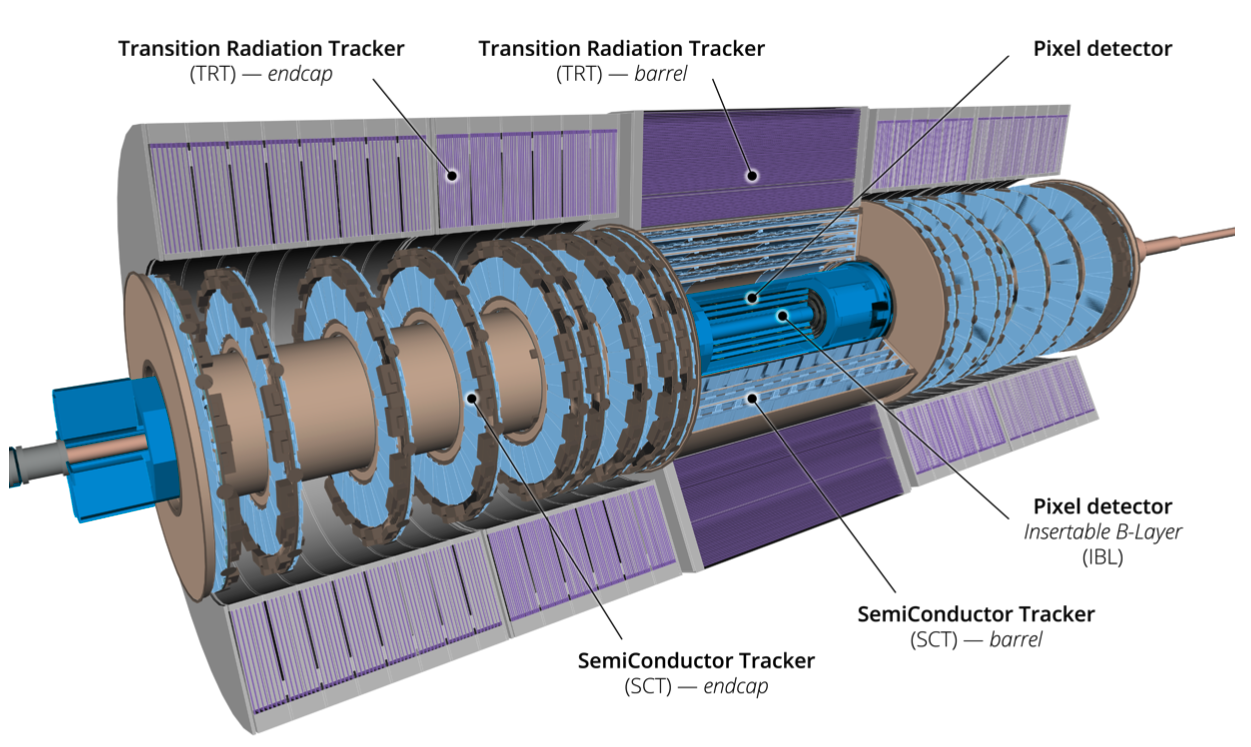
\includegraphics[width=.55\textwidth,keepaspectratio=true]{chapters/chapter3_experiment/images/ATLAS_ID_Run3.png}}
		% \subfloat[\label{fig:hpm-diagrams_b}]{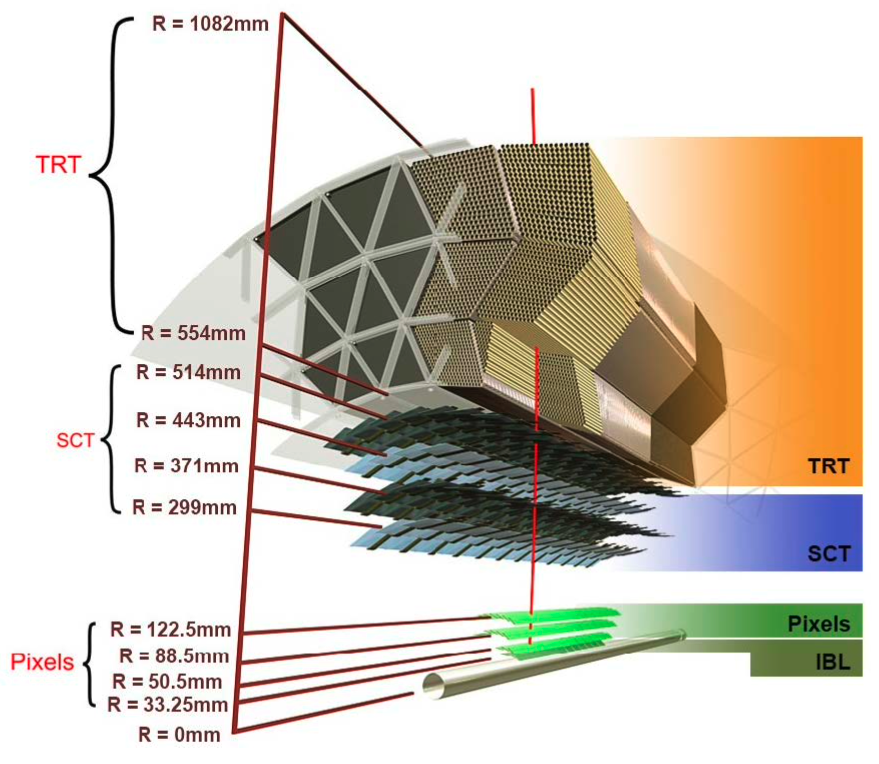
\includegraphics[width=.45\textwidth,keepaspectratio=true]{chapters/chapter3_experiment/images/ATLAS_ID_Transverse_View.png}}
		\subfloat[\label{fig:hpm-diagrams_a}]{\includegraphics[width=.55\textwidth,keepaspectratio=true]{chapters/chapter3_experiment/images/ATLAS_ID_Run2.jpg}}
		\subfloat[\label{fig:hpm-diagrams_b}]{\includegraphics[width=.45\textwidth,keepaspectratio=true]{chapters/chapter3_experiment/images/ATLAS_ID_Transverse_View_Run2.jpg}}
		\caption{\label{fig:ATLAS-ID} (a) Cut-away view of the \gls{ATLAS} Inner Detector. (b) Cross-sectional view of the ATLAS Inner Detector. \cite{atlas-schematics}}
		\end{figure}

		The \gls{ID} is the inner-most detector, closest to the \gls{IP} and is used to track the trajectory of charged particles leading to the measurement of electromagnetic charge and momentum. The \gls{ID} is immersed in the 2 T magnetic field provided by the central solenoid described in section \ref{sssec:solenoid} and covers a pseudorapidity range of $|\eta|<2.5$. The three subdetectors within the \gls{ID} can be seen in Figure \ref{fig:ATLAS-ID}, the Pixel, \gls{SCT}, and the \gls{TRT}. Like the toroid system, and many of the other subdetectors, the \gls{ID} is comprised of barrel and end-cap segments. The \gls{ID} barrel section is 1.6 m in length and covers $|\eta|<1$ while the end-caps measure over 7 m in length and cover $1 < |\eta| < 2.5$. 

		A track is considered good if there are hits in at least 3 pixel layers and 8 strips. The ID tracking system was designed with a resolution of 
		\begin{equation}\label{eqn:tracking-resolution}
		\frac{\sigma_{\pt}}{\pt} = 0.05 \% \, \pt \oplus 1\%
		\end{equation}
	
		\subsubsection{Pixel}\label{sssec:pixel}
			The detector closest to the beam and \gls{IP} is the Pixel Detector. The Pixel Detector is designed to measure particle hits with high-precision and high-granularity. The barrel Pixel detector consists of three layers of n-type silicon substrate with n-type implants. The closest layer to the \gls{IP} sits at 50.5 mm and the outermost layer extends out to 12 cm. This combination gives the Pixel Detector the ability to determine the impact parameters of collisions with incredible precision. Due to the high radiation dose this close to the \gls{IP}, the Pixel Detector was designed to be operated only in partial depletion. Each pixel cell measures $200 \mu m \times 400 \mu m \times 250 \mu m$. There are five Pixel disks on each end-cap of the \gls{ID}. In total there are 1,744 modules, with 46,080 readout channels per module, giving over 80 million channels with a spatial resolution of $10 \, \mu m (R-\phi) \times 115 \, \mu m (z)$ \cite{ATLAS-pixel}. 

			In order to keep up with the increased demand of Run-2 data taking conditions, an additional layer of pixels was installed in the Long Shutdown 1 (LS1) between 2013 and 2015. This \gls{IBL} provides even finer granularity tracking with pixel cells measuring $50 \, \mu m \times 250 \, \mu m$ installed at a radial distance of $R=33.25$ mm from the \gls{IP} and a spatial resolution of $8 \, \mu m (R-\phi) \times 40 \, \mu m (z)$ \cite{ATLAS-IBL}. The \gls{IBL} has proved incredibly useful in the reconstruction of displaced vertices from processes like \bjet hadronization and $\gamma \rightarrow e^+ e^-$.

		\subsubsection{Semiconductor Tracker}\label{sssec:SCT}
			Moving radially outward, the next subdetector is the \gls{SCT} that provides tracking in the intermediate radial range from the \gls{IP} and covers a range of $|\eta| < 2.5$. Similar to the Pixel Detector, the \gls{SCT} has 4 barrel layers and 9 end-cap wheels on each side. The \gls{SCT} provides four measurements per track via silicon microstrip detectors. Each microstrip is made of two $6.36 \times 6.40 \, cm^2$ detectors glued end to end so each microstrip is $12.8 \, cm$ long. Two microstrips are then glued back to back with a $40 \, \mu rad$ angle. In total there are 768 strips, giving 6.2 million readout channels. The \gls{SCT} has a spatial resolution of $17 \, \mu m (R-\phi) \times 580 \,\mu m (z)$ and can distinguish tracks with as small as a $200 \, \mu m$ separation \cite{ATLAS-ID}.

		\subsubsection{Transition Radiation Tracker}\label{sssec:TRT}
			The final subdetector of the \gls{ID} is the \gls{TRT} $(R=554 \, \mathrm{mm} \, - 1082 \, \mathrm{mm})$ . Instead of silicon detectors the \gls{TRT} uses 4 mm diameter straw tubes; a hollow tube with a sense wire that is held at high voltage in the middle. The maximum length of a straw is 150 cm. The straws are filled with a gaseous mixture of $70\% \, \mathrm{Xe,} \, 27\% \, \mathrm{CO}_2, \, 3\% \, \mathrm{O}_2$.\footnote{During Run-2 the Xe was replaced with Ar as a cost saving measure. Ar provides similar performance as Xe in tracking, but is less efficient in absorbing X-rays from transition radiation.} Charged particles ionize the gas mixture, thereby releasing an electron and an ion. The ion drifts to the straw surface and the electron drifts to the wire; this charge drift is then measured as a signal. The \gls{TRT} checks the signals against two thresholds, a lower threshold for measuring the drift time to derive a position and a higher threshold that is used to identify transition radiation X-rays. Transition radiation occurs when a charged particle hits the boundary of two media with differing dielectric constants; in the case of the \gls{TRT} the two media are the gas and the straw tube. The higher threshold provides discriminating power between charged pions and electrons.

			The \gls{TRT} consists of a barrel section and 18 wheels in each end-cap. In the barrel, there are 50,000 straws divided in two at the center to allow for two separate readouts. The end-caps have 320,000 straws. In total, there are 420,000 readout channels. Each straw provides a spatial resolution of $170 \mu m$. \cite{ATLAS-ID}

	\subsection{Calorimeters}\label{ssec:calorimeters}
		The ATLAS detector makes use of two types of sampling calorimeters, one that uses liquid argon as the active medium and another that uses scintillating plastic tiles. Both types of calorimeters are designed to fully absorb particles via showering. Incoming particles interact with an absorber material and generate secondary particles. Those secondary particles interact with the absorber and create another set of particles. This cascading effect creates showers of particles inside the calorimeters. The shape and depth of these particles is important in the design choices for the calorimeters as well as particle identification. Two helpful variables when talking about shower depth are radiation length $\chi_0$ and nuclear interaction length $\lambda$. $\chi_0$ is defined as the distance where a particle has lost energy via bremsstrahlung equal to $\frac{1}{e}$\footnote{$\chi_0$ can also be defined as $\frac{7}{9}$ of the mean free path of a high energy photon.}, whereas $\lambda$ is the mean free path of a hadron before undergoing a inelastic nuclear interaction. In order to fully absorb a wide energy range of incident particles the calorimeters are designed such that any path through them is at least $25 \, \chi_0$ or $10 \, \lambda$. Figure \ref{fig:calo-interaction-length} shows the calorimeter layers and their nuclear interaction lengths as a function of $\eta$.

		\begin{figure}[!ht]
		\centering
		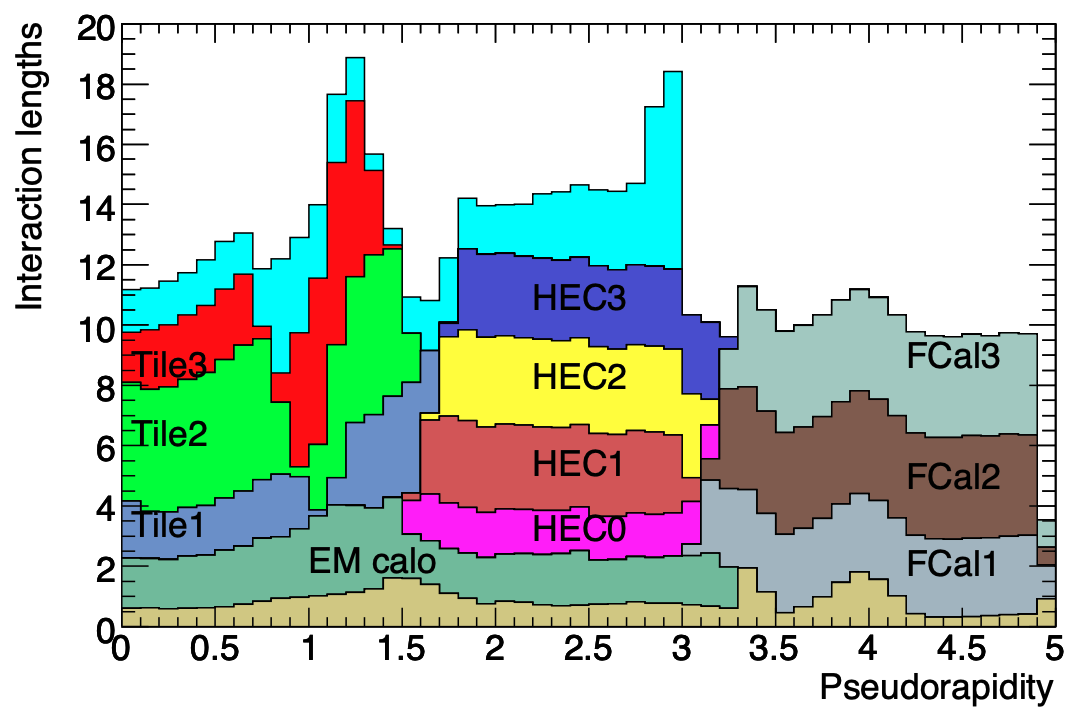
\includegraphics[width=.65\textwidth,keepaspectratio=true]{chapters/chapter3_experiment/images/Calo_Interaction_Lengths.png}
		\caption{ Interaction lengths as a function of $\eta$ in the \gls{ATLAS} calorimeters. The unlabeled brown color is the material in front of the EM calorimeters and the unlabeled cyan is the amount of material in front of the first active layer of the muon spectrometer. \cite{atlas-experiment}}
		\label{fig:calo-interaction-length}
		\end{figure}

		The design resolution of the calorimeters can be seen in Table \ref{tab:calo-resolution}.

		\begin{table}[!thp]
		\centering
		\caption{ Design resolution of EM and hadronic calorimeters in the \gls{ATLAS} Detector.}
		\resizebox{.45\textwidth}{!}{\begin{tabular}{| c | c | c |}  
		\hline
		Calorimeter											& Pseudorapidity range 																		& Resolution \\[1ex] \hline 
		Electromagnetic 									& $| \eta | < 3.2$ 																			& $\frac{\sigma}{E} = \frac{10\%}{\sqrt{E}} \oplus 0.7\%$ \\[1ex] \hline
		\multicolumn{1}{|c|}{\multirow{2}{*}{Hadronic}} 	& \begin{tabular}[c]{@{}c@{}} $| \eta | < 3.2$ \\[1ex] $3.1 < | \eta | < 4.9$ \end{tabular} & \begin{tabular}[c]{@{}c@{}} $\frac{\sigma}{E} = \frac{50\%}{\sqrt{E}} \oplus 3\%$ \\[1ex] $\frac{\sigma}{E} = \frac{100\%}{\sqrt{E}} \oplus 10\%$ \end{tabular} \\ \hline 
		\end{tabular}}
		\label{tab:calo-resolution}
		\end{table}

		The layout of calorimeters in the \gls{ATLAS} detector can be seen in Figure \ref{fig:calo-layout}.
		\begin{figure}[!ht]
		\centering
		% 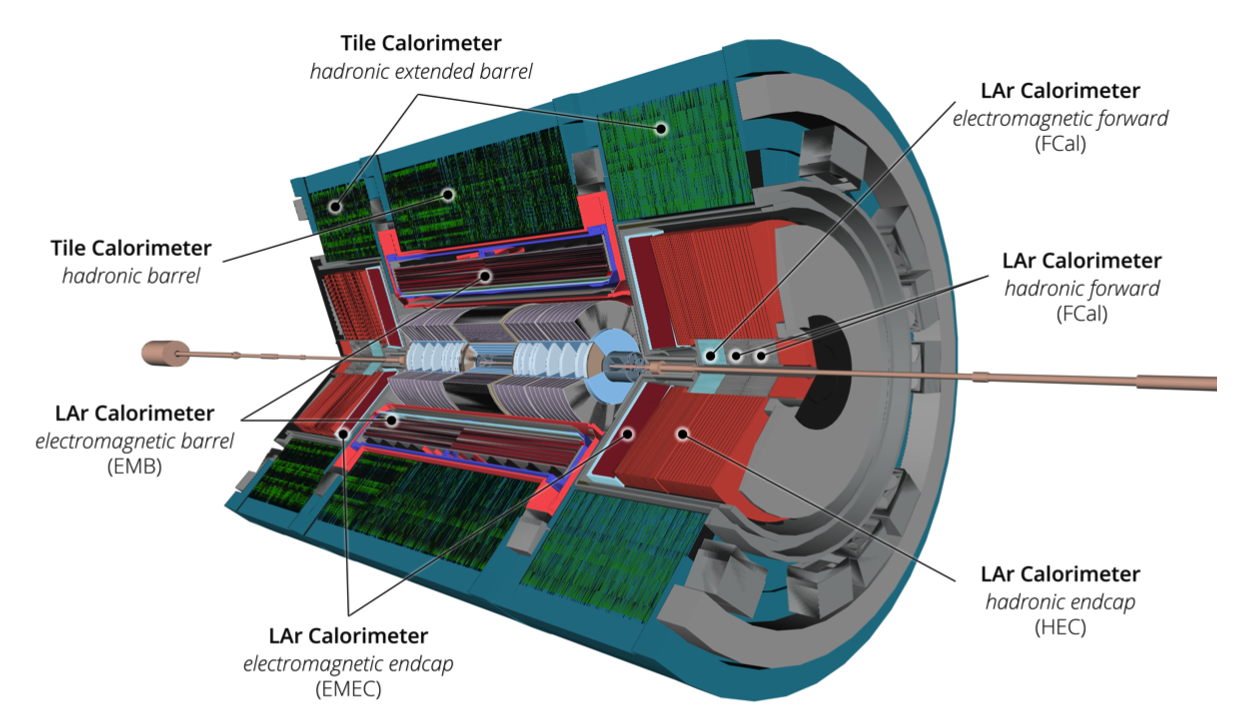
\includegraphics[width=.85\textwidth,keepaspectratio=true]{chapters/chapter3_experiment/images/ATLAS_Calorimeters_Run3.png}
		\includegraphics[width=.85\textwidth,keepaspectratio=true]{chapters/chapter3_experiment/images/ATLAS_Calorimeters_Run2.jpg}
		\caption{ Cut-out view of the \gls{ATLAS} detector's calorimeters. \cite{atlas-schematics}}
		\label{fig:calo-layout}
		\end{figure}

		\subsubsection{Liquid Argon Calorimeters}\label{sssec:LAr}
			The \gls{LAr} calorimeters are based on a similar principle to the straw tubes of the \gls{TRT} described in section \ref{sssec:TRT}. In this case, the \gls{LAr} is the active medium that is ionized by the incoming particle. The free electron then drifts to an electrode, copper-tungsten in the case of the barrel \gls{LAr} calorimeter. The drifting electrons are then readout as an electrical signal; there are approximately 180,000 \gls{LAr} readout channels in the \gls{ATLAS} detector. \gls{LAr} was chosen as the active medium due to it's intrinsic radiation hardness, stability over time, and linear response. The \gls{LAr} must be kept at very cold temperatures, around 85 K. To achieve this, the \gls{LAr} calorimeters are kept in cryostats, the barrel calorimeter shares the cryostat and vacuum with the central solenoid.

			There are four \gls{LAr} calorimeters within the \gls{ATLAS} detector. The \gls{EMB} is designed for electromagnetic calorimetry with a lead-stainless steel absorber and covers a pseudorapidity range of $|\eta|<2.5$. Next in $\eta$ is the \gls{EMEC} that also uses lead-stainless steel absorber and the \gls{LAr} Hadronic End-Cap (HEC) which has a copper plate absorber; both \gls{EMEC} and \gls{HEC} cover $1.5 < |\eta| < 3.2$. The final \gls{LAr} calorimeter is the aptly named \gls{FCAL} that covers $|\eta|<4.9$ and has three modules. The first is optimized for \gls{EM} calorimetry and uses a copper absorber. The other two \gls{FCAL} modules are used to measure hadronic showers and use tungsten absorbers.

			The \gls{EMB} and \gls{EMEC} both utilize an accordion geometry pictured in Figure \ref{fig:LAr-accordion} to ensure a full $\phi$ coverage. 
			\begin{figure}[!ht]{}
			\centering
			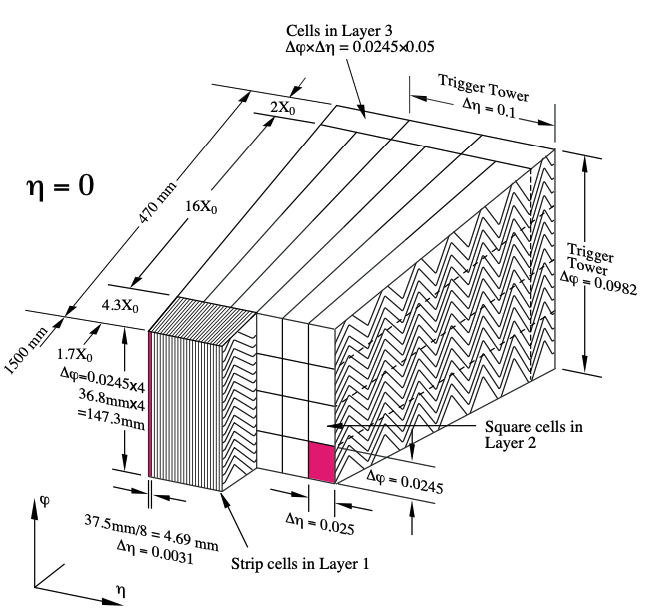
\includegraphics[width=.45\textwidth,keepaspectratio=true]{chapters/chapter3_experiment/images/LAr_Accordion_Geometry.png}
			\caption{An \gls{EMB} module showing the accordion geometry and granularity. \cite{LAr-TDR}} %\cite{atlas-experiment}}
			\label{fig:LAr-accordion}
			\end{figure}
			The \gls{EMB} consists of four layers, the first being a \gls{LAr} presampler of 1.1 cm thickness. The presampler is used to correct for energy losses due to material in front of the calorimeter. The first layer after the presampler is finely segmented to ensure good position measurements. The second layer is $16 \, \chi_0$ thick and collects most of the electromagnetic showers. Typically, only the tails of \gls{EM} showers make it to the third and final layer, so a coarser granularity is used. 

		\subsubsection{Tile Calorimeter}\label{sssec:Tile}
			\begin{figure}[!ht]
			\centering
			\subfloat[\label{fig:tile-modules_a}]{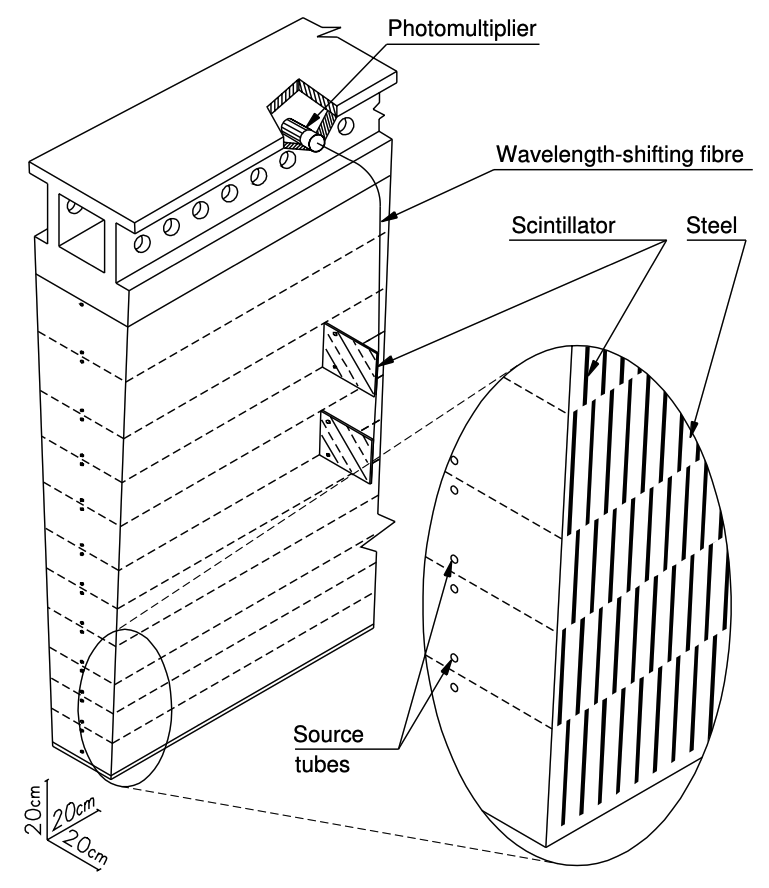
\includegraphics[width=.45\textwidth,keepaspectratio=true]{chapters/chapter3_experiment/images/TileModuleCrossSection.png}} \\
			\subfloat[\label{fig:tile-modules_b}]{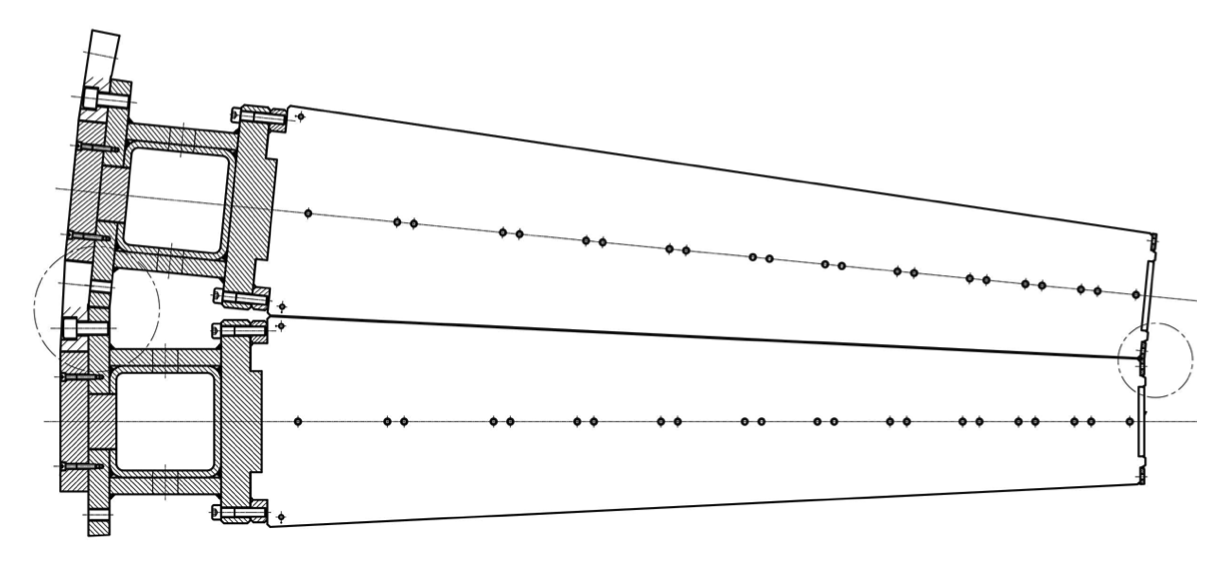
\includegraphics[width=.45\textwidth,keepaspectratio=true]{chapters/chapter3_experiment/images/Tile_Modules_Azimuth_View.png}}
			\caption{\label{fig:tile-modules} (a) Diagram of an individual \gls{TileCal} module. (b) Azimuthal view of two \gls{TileCal} modules with the \gls{IP} being to the right. \cite{ATLAS-tile}}
			\end{figure}
			The hadronic \gls{TileCal} is a sampling calorimeter that is designed to fully absorb hadronic showers covering a range of $|\eta|<1.7$ at a radial distance of $2.28 \, \mathrm{m} \leq R \leq 4.25 \, \mathrm{m}$ from the \gls{IP}. This radial distance translates to approximately $7.4\, \lambda$. A similar design of absorber and electrode is used in \gls{TileCal} to capture the full energy of hadronic showers. \gls{TileCal} uses a steel absorber. However, instead of a liquid or gas being ionized and the free electrons being collected as a signal, \gls{TileCal} takes advantage of a special material called scintillating plastic. When an ionizing particle interacts with the scintillating plastic, light is created; this light is absorbed in wavelength shifting fibers. It is then re-emitted and transmitted to \glspl{PMT}. The \gls{PMT} signal is then shaped, amplified at two gains with a ratio of 64:1, then digitized at 40 MHz with 10-bit analogue-to-digital converters. Each cell within \gls{TileCal} has 2 \glspl{PMT}, giving over 10,000 readout channels. There are 256 modules within \gls{TileCal}. A diagram of an individual module and the layout of two modules side-by-side can be seen in Figure \ref{fig:tile-modules}.
			

			A significant fraction of the author's time and effort during their PhD went to data quality monitoring and maintenance of \gls{TileCal}. These works are detailed in Appendix \ref{app:Tile-DQ}.

	\subsection{Muon Spectrometer}\label{ssec:muon-system}
		High momentum muons provide a vital signature at the LHC. Muons are minimally ionizing particles, meaning they leave a small amount of energy inside detectors and travel to the edge and beyond the volume of the \gls{ATLAS} detector. Instead of attempting to fully absorb muons, high precision position measurements are taken to track their trajectories. The toroid magnet system described in Section \ref{sssec:toroid} is an integral part of the \gls{MS}; it provides the bending force, changing the trajectories to the direction of the beamline. The barrel section of the \gls{MS} consists of three concentric cylindrical shells at $R=5 \, \mathrm{ m, }\, 7.5 \, \mathrm{ m, } \,  10 \, \mathrm{ m}$ made of \glspl{MDT} $(|\eta|<1)$. \cite{ATLAS-muon} These cylindrical shells sit in-between and on the air core toroid magnets. On the $2^{\mathrm{nd}}$ and $3^{\mathrm{rd}}$ shells are \glspl{RPC} that provide quick triggering. Complimenting the barrel section are the end-caps, referred to as wheels for the \gls{MS}. The wheels are placed at $|z|\approx 7.4 \, \mathrm{ m, } \, 10.8 \, \mathrm{ m, } \, 14 \, \mathrm{ m, and} \,21.5 \,\mathrm{ m }$ $(2.0 < |\eta| < 2.7)$. The innermost layer of these wheels experience the highest rates of incident particles. To cope with this, \glspl{CSC} with a finer granularity than the \glspl{MDT} that are used in the barrel. Similarly, \glspl{TGC} are used for triggering instead of \glspl{RPC}. These wheels provide spatial coordinates orthogonal to those of the precision-tracking \glspl{MDT} in the barrel. Figure \ref{fig:muon-spec} shows the positioning of the various \gls{MS} components.
		% \footnote{Figure \ref{fig:muon-spec} Shows the \gls{NSW}. The \gls{NSW} is an upgrade to the old Small Wheels that were used in the data taking period that concerns this dissertation.}

		% \begin{figure}[!h]
		% \centering
		% \subfloat[\label{fig:muon-spec_a}]{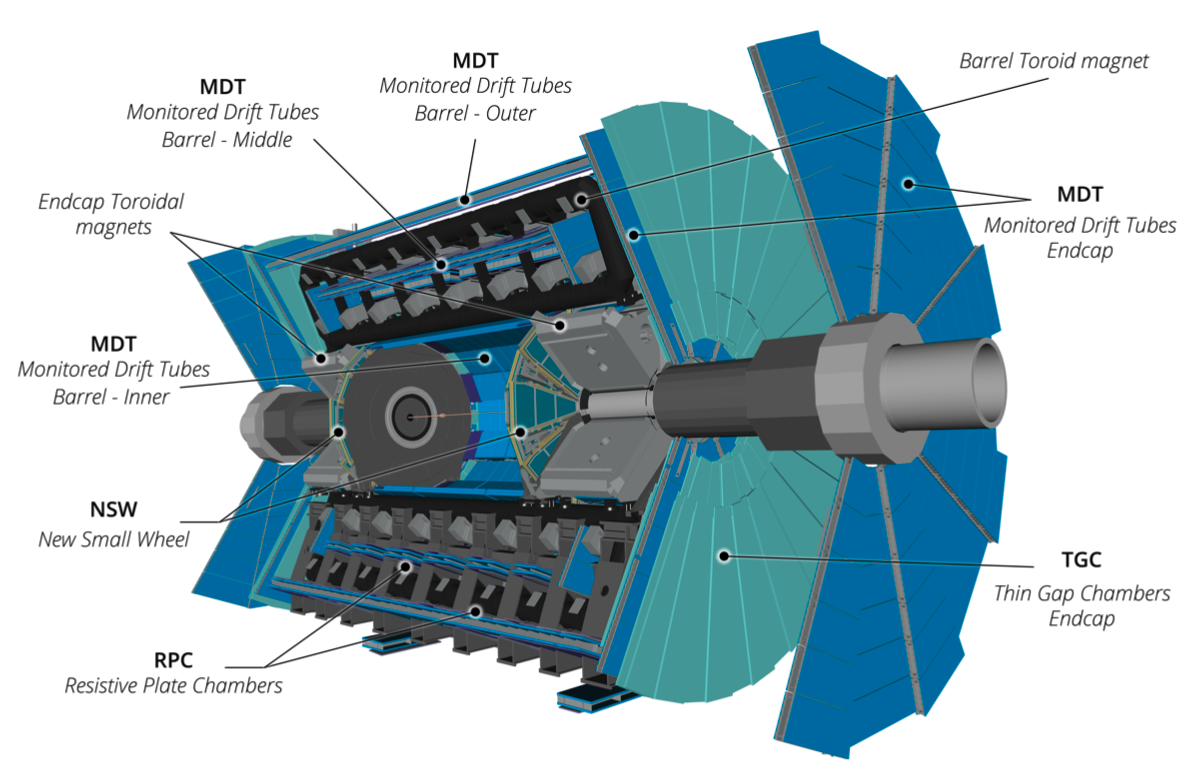
\includegraphics[width=.45\textwidth,keepaspectratio=true]{chapters/chapter3_experiment/images/ATLAS_Muon_System_Run3.png}}
		% \subfloat[\label{fig:muon-spec_b}]{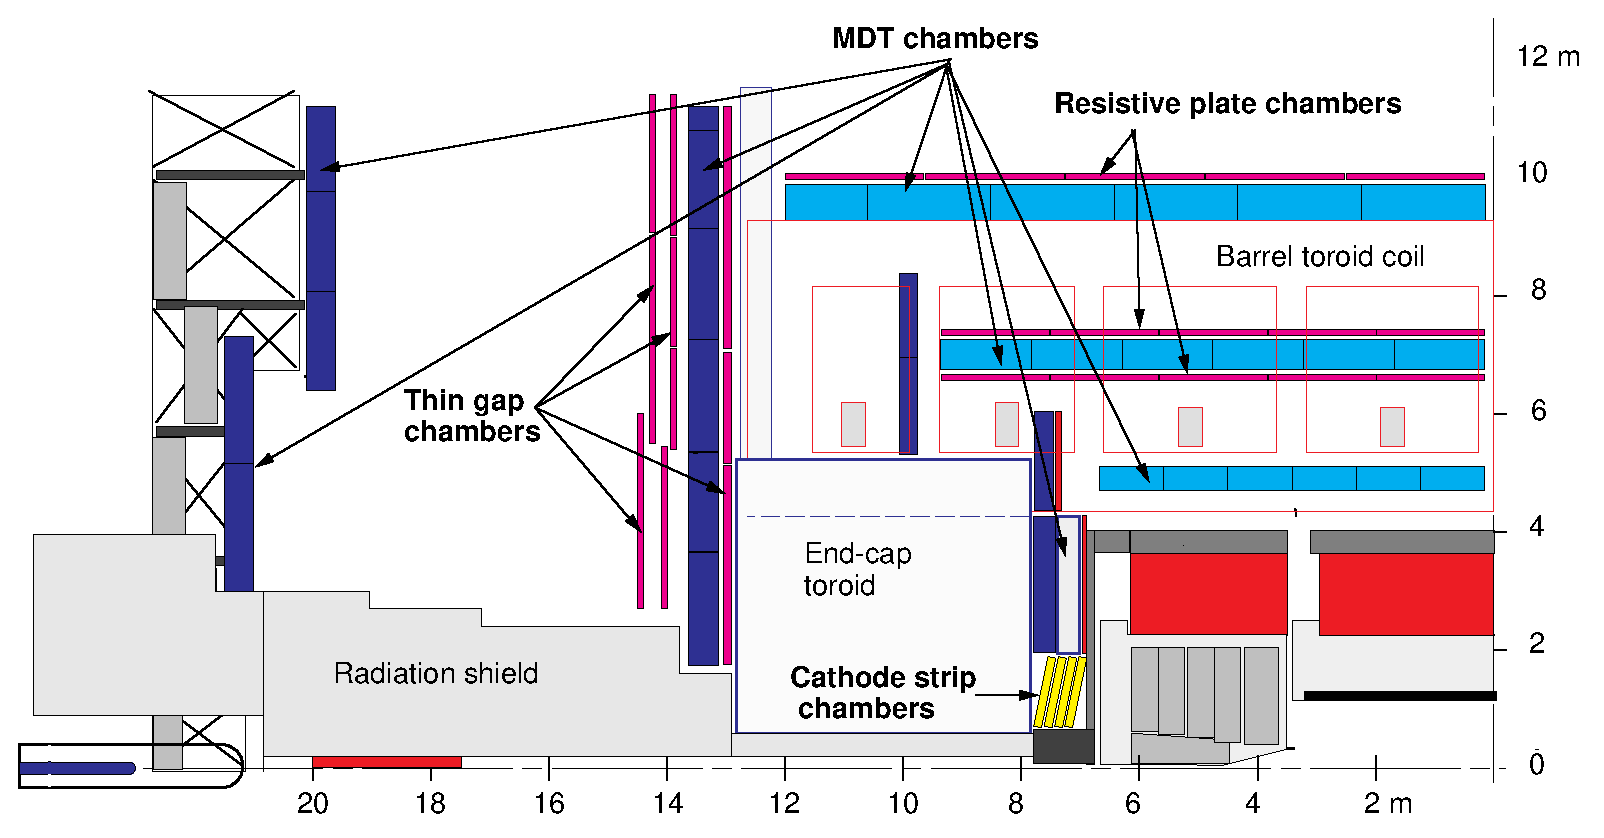
\includegraphics[width=.45\textwidth,keepaspectratio=true]{chapters/chapter3_experiment/images/ATLAS-muon-rz-tdr.eps}} \\
		% \subfloat[\label{fig:muon-spec_c}]{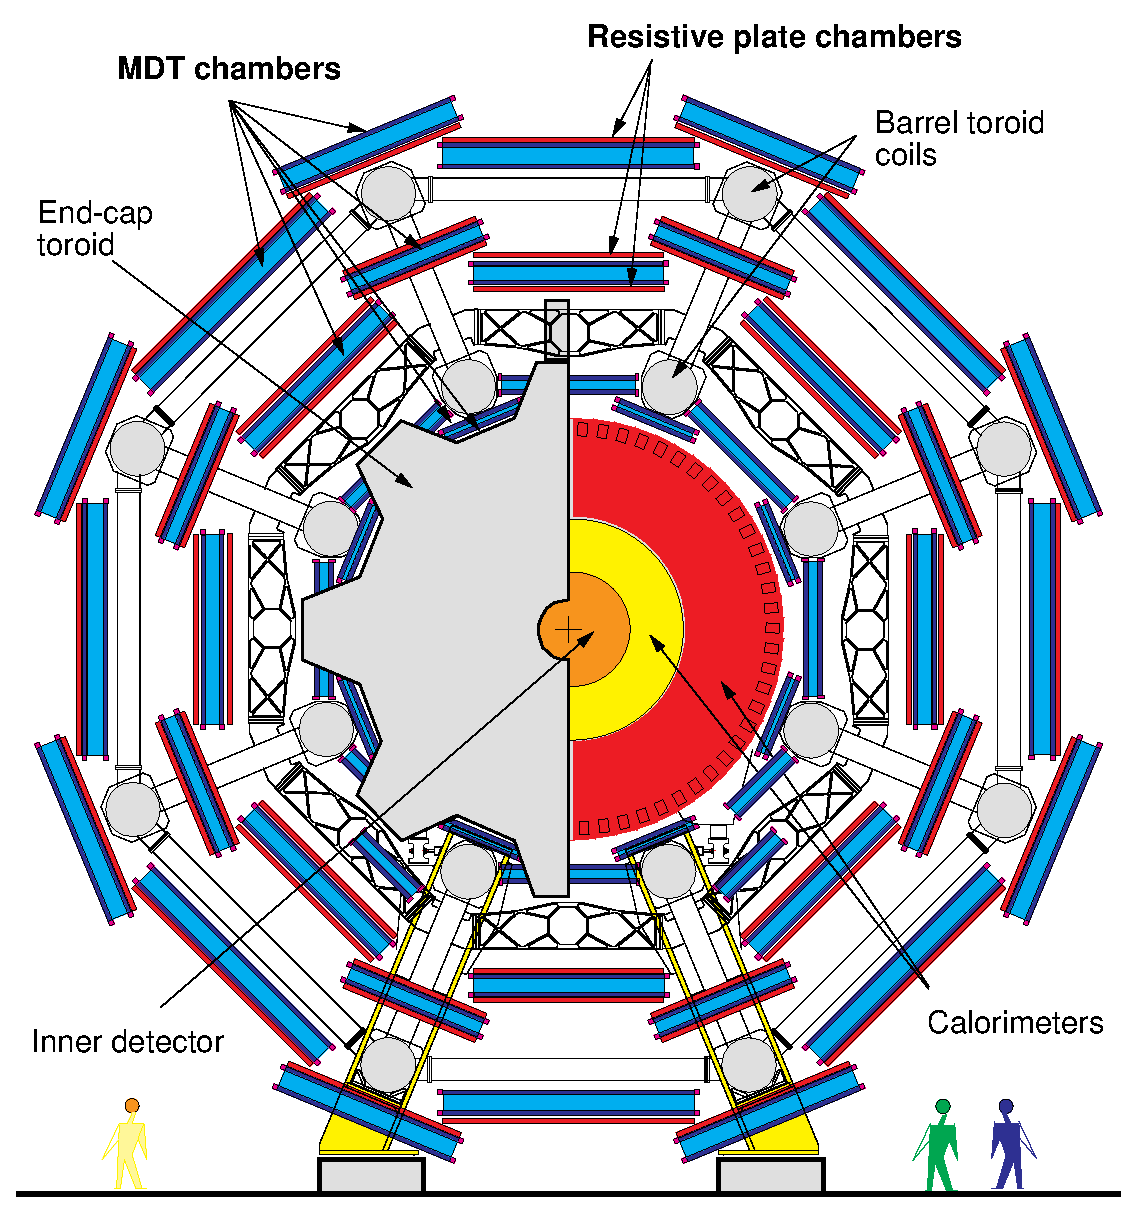
\includegraphics[width=.45\textwidth,keepaspectratio=true]{chapters/chapter3_experiment/images/ATLAS-muon-xy-tdr.eps}}
		% \caption{\label{fig:muon-spec} (a)   (b)}
		% \end{figure}

		\begin{figure}[!ht]
		\centering
		% 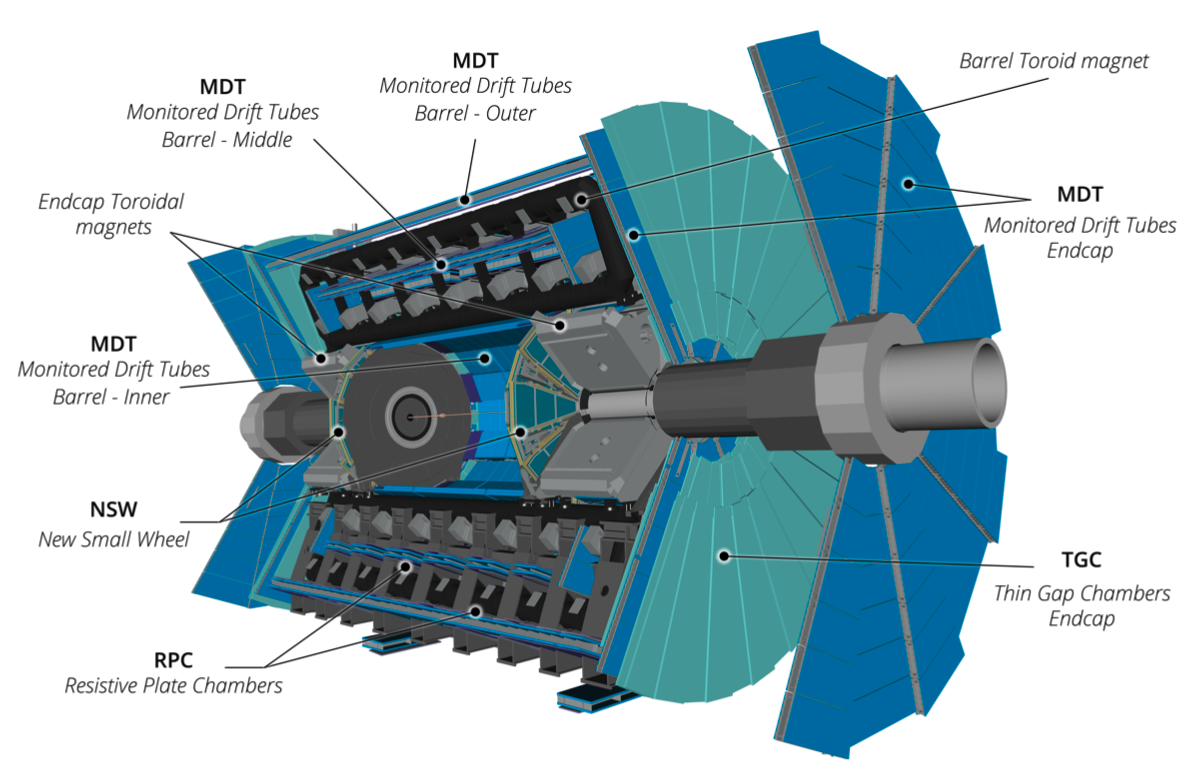
\includegraphics[width=\textwidth,keepaspectratio=true]{chapters/chapter3_experiment/images/ATLAS_Muon_System_Run3.png}
		\includegraphics[width=\textwidth,keepaspectratio=true]{chapters/chapter3_experiment/images/ATLAS_Muon_System_Run2.png}
		\caption{Cut-out view of the \gls{ATLAS} detector Muon Spectrometer. \cite{atlas-schematics}}
		\label{fig:muon-spec}
		\end{figure}

	\subsection{Trigger System}\label{ssec:trigger}
		The large luminosity provided by the \gls{LHC} is critical in collecting enough data to make detailed physics analyses. However, it also means that there is an incredibly large amount of data to sort through. So much that it is not possible to write out the data from every bunch crossing. As shown in Figure \ref{fig:high-pileup-event-display}, even one single event can contain an inordinate amount of data. Another issue arises due to the nature of hadron collisions; in that not all bunch crossing provide hard scatter inelastic collisions that are ``interesting'' enough to save data on. 

		To solve this issue, the data coming out of \gls{ATLAS} is combed through in real time at a variable rate of 1 kHz to 40 MHz. This is done with a \gls{TDAQ} system. The \gls{TDAQ} system used in Run-2 is described in detail Reference \cite{ATLAS-trigger-Run2}. The \gls{TDAQ} system reads in data from the \gls{ATLAS} detector, calculates relevant quantities, and makes a decision on if there was an event worth storing. A diagram showing the data flow into the \gls{TDAQ} system is show in \ref{fig:trigger-run2}.\footnote{Figure \ref{fig:trigger-run2} shows the Fast TracKer (FTK). During Run 2 FTK was undergoing commissioning and was not used in the active \gls{TDAQ} system.} 
		\begin{figure}[!ht]
		\centering
		% 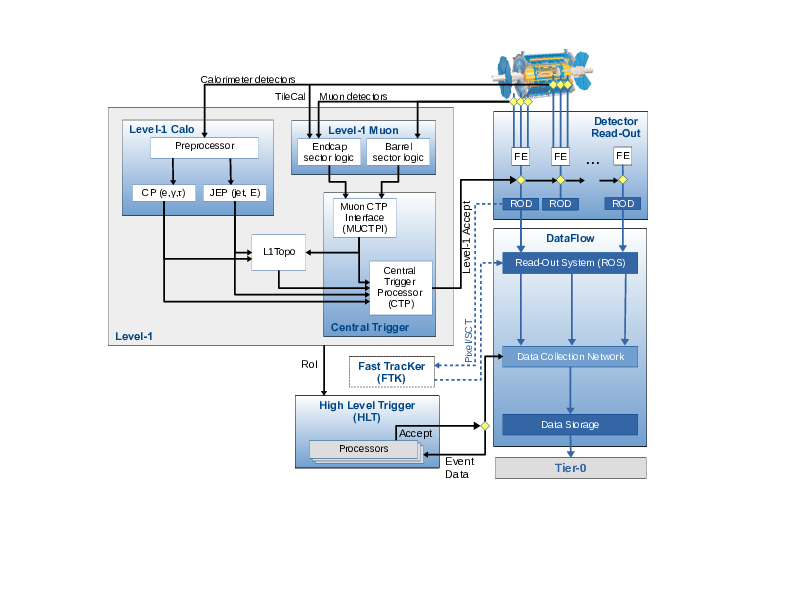
\includegraphics[width=\textwidth,keepaspectratio=true]{chapters/chapter3_experiment/images/Trigger_Run2.png}
		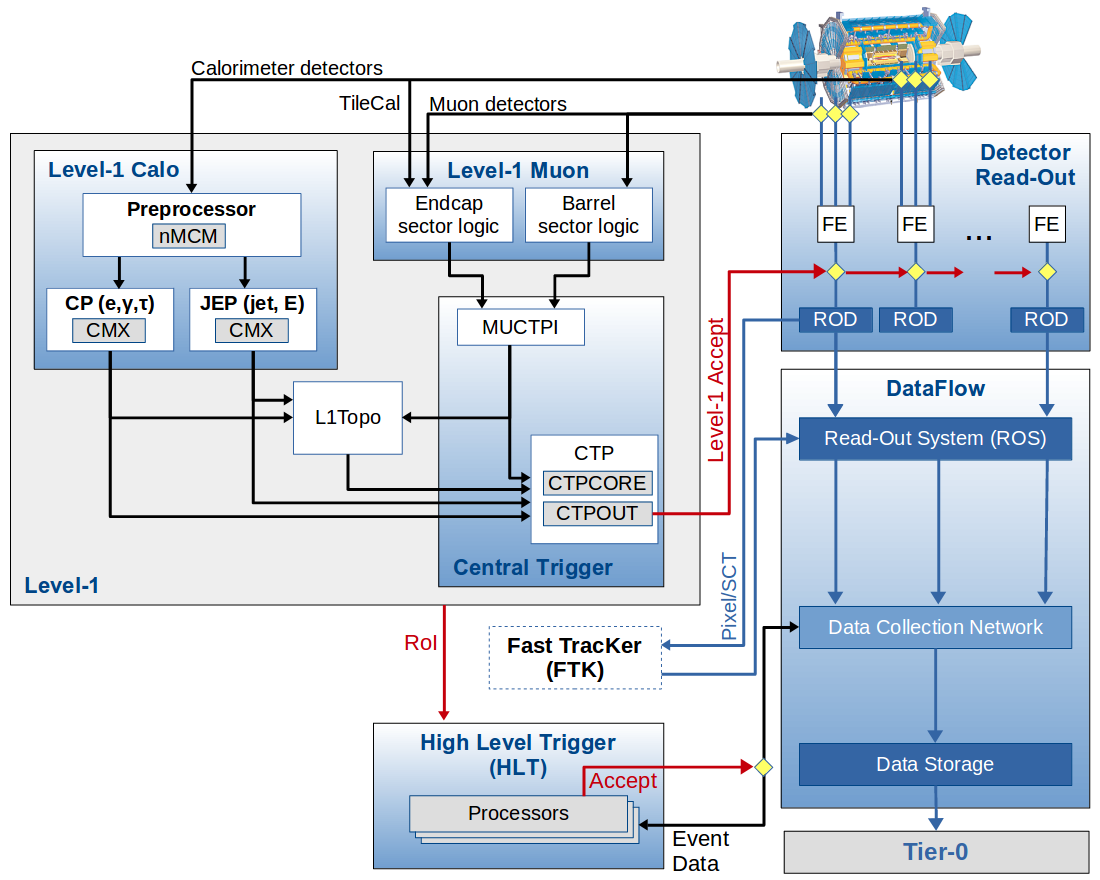
\includegraphics[width=\textwidth,keepaspectratio=true]{chapters/chapter3_experiment/images/tdaq-run2-schematic2017.png}
		\caption{The \gls{ATLAS} \gls{TDAQ} system in Run-2 showing the components relevant for triggering as well as the detector read-out and data flow. \cite{TDAQ_Diagram}}
		\label{fig:trigger-run2}
		\end{figure}
		The \gls{ATLAS} \gls{TDAQ} system consists of two main components, \gls{L1} and \gls{HLT}. The \gls{L1} is a hardware based trigger system that reads in data from the calorimeters and muon spectrometer. The \gls{L1} has a latency of $2.5 \, \mu \mathrm{s}$ and can read-out accepted events up to 100 kHz, the detector maximum readout rate. The \gls{HLT} is a software based trigger system based on the offline reconstruction software. During Run-2 the \gls{HLT} operated with an average output rate of 1.2 kHz, which translates to about 1.2 GB/s of data sent to permanent storage.	

		After the \gls{TDAQ} system accepts an event, the data is set to be stored on magnetic tape for long term storage. It is also processed at the local computing farm named Tier-0 with the full reconstruction software suite described in Chapter \ref{chap:reco}.


\chapter{Simulation}\label{chap:sim}
	The data collected by the \gls{ATLAS} experiment must be compared to a well understood dataset. This dataset is most often a dataset of simulation particle collisions that aim to mimic physics processes and particle interaction with detector material, as well as the detector's response. Figure \ref{fig:simulation} shows the chain of simulations by which these datasets are produced.
	\begin{figure}[!ht]
	\centering
	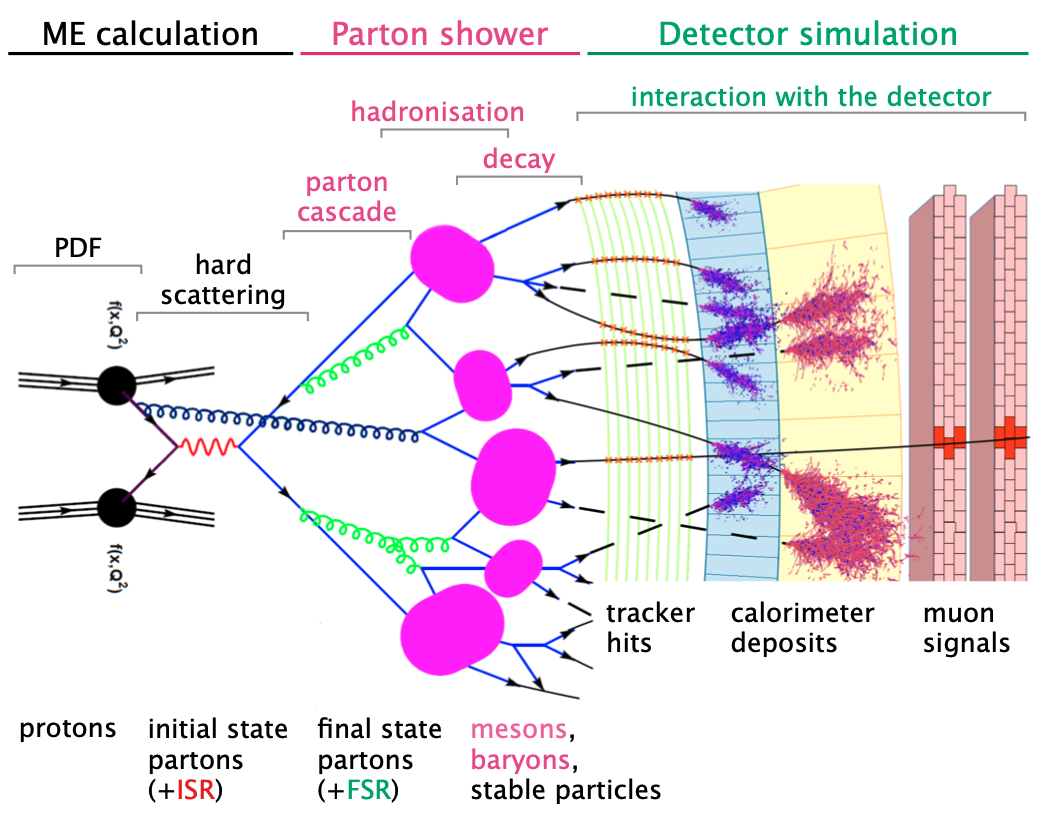
\includegraphics[width=.95\textwidth,keepaspectratio=true]{chapters/chapter4_simulation/images/Simulation_Chain.png}
	\caption{\label{fig:simulation} A pictorial representation of the simulation chain used in the \gls{ATLAS} experiment \cite{Wanotayaroj:2242196}.}
	\end{figure}
	
	Many particle physics experiments, \gls{ATLAS} included, use \gls{MC} simulation techniques to produce these datasets. Monte Carlo simulation techniques use repeated random sampling of underlying probability density functions to closely model various processes. 

	\section{Event Generation and Hadronization}\label{sec:event-gen}
		Since protons and other hadrons are not fundamental particles, it is impossible to know the exact constituents (partons) that interacted during a collision. To mimic this intrinsic probabilistic nature, \acrfullpl{PDF} are used. A \gls{PDF} models the probability of any parton within a proton (or hadron) to carry a fraction of the beam energy at a given hadron momentum. The \gls{PDF} and subsequent inelastic hard scattering of the interacting partons are modeled via a \gls{ME} calculation, which can be depicted through Feynman diagrams. This \gls{ME} calculation is done to fixed order in perturbation theory, \gls{LO}, \gls{NLO}, \gls{LL}, etc. This first level event generation can be done by a myriad of \gls{MC} event generators. Often specific choices are made based on individual generator performance for a given physics process.

		The next step in the simulation chain is the parton showering and hadronization. This can be done with a different set of \gls{MC} simulations. Parton showering and hadronization are complex, computationally expensive steps to simulate and are done iteratively. An example of a parton shower generator output can be seen in Figure \ref{fig:hadronization}.

		The \gls{MC} generators used in this dissertation for background simulations are Pythia \cite{pythia}, Powheg-Box \cites{powheg-1}{powheg-2}, and Sherpa \cite{sherpa}. For signal, MadGraph is used \cite{MadGraph}. For all processes, Pythia8 is used to simulate the parton shower, fragmentation, and underlying event. Table \ref{tab:bkg-generators} shows which \gls{MC} generator is used for each background process.

				\begin{table}[!thp]
			\begin{center}
			\small
			\resizebox{0.5\textwidth}{!}{
			\begin{tabular}{|c||c|}
			\hline
			Background process & Generator \& parton shower  \\
			\hline \hline
			\ttbar with at least one lepton $\ell$ 	& 	Powheg \& Pythia8 	\\ \hline
			Single top-quark 						& 	Powheg \& Pythia8 	\\ \hline
			W ($\ell \nu$) + jets 					& 	Sherpa 				\\ \hline
			Z/$\gamma^{*}(\ell \ell , \nu \nu)$ + jets &Sherpa 				\\ \hline
			$WW$ 									& 	Powheg \& Pythua8 	\\ \hline
			$WZ$ 									& 	Powheg \& Pythua8 	\\ \hline
			$ZZ$ 									& 	Powheg \& Pythua8 	\\ \hline

			\end{tabular}}
			\normalsize
			\caption{\label{tab:bkg-generators}
			\gls{MC} generators for the main \acrshort{SM} background samples at \sqs. 
			Here, $\ell$ refers to the three lepton families $e$, $\mu$ and 
			$\tau$.
			}
			\end{center}
		\end{table}

		\begin{figure}[!ht]
		\centering
		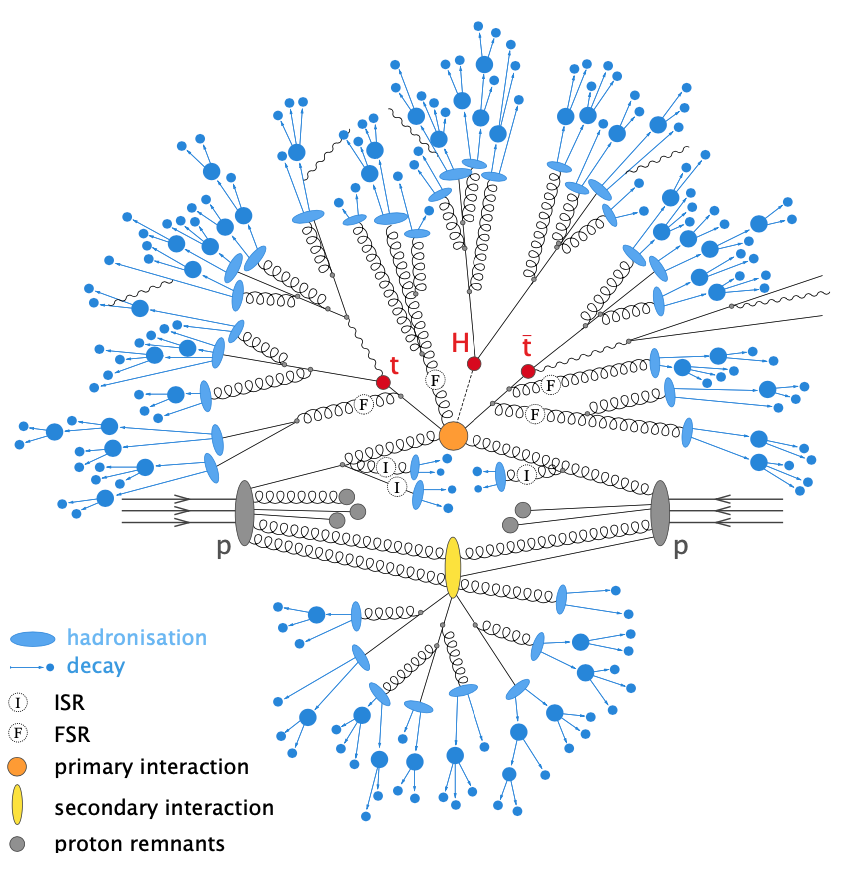
\includegraphics[width=\textwidth,keepaspectratio=true]{chapters/chapter4_simulation/images/tth_hadronization_gen.png}
		\caption{\label{fig:hadronization} A pictorial representation of a parton shower of a t$\bar{\mathrm{t}}$H event \cite{Wanotayaroj:2242196}.}
		\end{figure}	

	\section{Detector Simulation}\label{sec:detector-sim}
		The final step in the simulation chain is simulating the particle's interaction with the detector material and the detector's response. Up until this point, the \gls{MC} generators used are generic non-experiment dependent simulations. The \gls{ATLAS} collaboration uses a GEANT4 based generator suite to simulate these interactions \cite{GEANT4}. These detailed simulations include all support structure, material densities, readout electronics, and digitization in order to fully simulate the path of a real particle through the \gls{ATLAS} detector. These simulations are often too slow to produce enough statistics for physics analyses. In the full simulation, around $80\%$ of the simulation time is spent on particles traversing the calorimeters and $75\%$ is spent on electromagnetic particles alone \cite{ATLAS-simulation}. Instead, several methods were developed to speed up the simulation known as FAST simulations. A detailed description of the \gls{ATLAS} simulation chain and options can be seen in Reference \cite{ATLAS-simulation}. The final simulated dataset is output into a raw data format identical to real data coming off of the \gls{ATLAS} detector. 

		
\chapter{Event Reconstruction}\label{chap:reco}
	Before any physics analysis can be performed on the raw data from the ATLAS detector and MC simulations both raw datasets go through a reconstruction software suite called Athena. Various algorithms are employed to identify energy deposits as particles based on shower shapes, tracker hits, calculated charge to mass ratios, etc. Figure \ref{fig:ATLAS-XSec} shows the signatures of various particles within the ATLAS detector. 

	\begin{figure}[!ht]
	\centering
	\includegraphics[width=.65\textwidth,keepaspectratio=true]{chapters/chapter3_experiment/images/ATLASCrossSectionDiagram.png}
	\caption{ Cross section view of the ATLAS detector with subdetectors labeled. Various types of particles radial trajectories are shown.}
	\label{fig:ATLAS-XSec}
	\end{figure}

	The following sections detail the identification processes of muons, electrons, photons, jets, $\tau$ leptons, and a calculated quantity called missing transverse energy (\Etm). These reconstructed physics objects are the inputs to the majority of physics analyses.

	\section{Tracks}
	Tracks are fits connected three dimensional space-points in the ID. These space-points are created from clusters of hits in the ID. A set of three space-points are combined into one track seed, then fed into three methods in the ATLAS detector: inside-out,  outside-in, and TRT-standalone. The inside-out method creates tracks by starting with a seed hit in the pixel detector, then SCT hits are added, finally the track is extrapolated out into the TRT. This method creates tracks of particles that are mostly produced in the hard \pp interaction and has a requirement of $\pt>400$ MeV. On the other-hand the outside-in method starts with track segments in the TRT and extrapolates towards the beamline using silicon that were not used in the inside-out method. Outside-in tracking typically reconstructs secondary vertices from particles that have long enough lifetimes to decay while inside the ID, including b quarks and $\tau$ leptons. Lastly, TRT-standalone tracks are made only from seeds within the TRT and are not extrapolated to the silicon subdetectors  \cite{ATLAS-perf-run2}. The reconstructed tracks are used in the identification of various types of particles.

	% Reconstructed tracks are made at two working points (WPs) to give analyzers a variety of track fits to best fit the analysis' needs
	% \begin{multicols}{2}
	% \begin{itemize}
	% 	\item Loose
	% 	\begin{itemize}
	% 		\item $\pt > 400$ MeV
	% 		\item $|\eta|<2.5$
	% 		\item $\geq 7$ silicon hits
	% 		\item $\leq 1$ shared modules
	% 		\item $\leq 2$ silicon holes
	% 		\item $\leq 1$ pixel holes
	% 	\end{itemize}
	% 	\item Tight
	% 	\begin{itemize}
	% 		\item if $|\eta|<1.65$
	% 		\begin{itemize}
	% 			\item $\geq 9$ silicon hits
	% 		\end{itemize}
	% 		\item if $|\eta| > 1.65$
	% 		\begin{itemize}
	% 			\item $\geq 11$ silicon hits
	% 			\item 1 hit on 2 innermost pixel layers
	% 			\item 0 pixel holes
	% 		\end{itemize}
	% 	\end{itemize}
	% \end{itemize}	

	% \end{multicols}

	\section{Topological Clusters}
	A topocluster is defined as a cluster of topologically connected calorimeter cell signals. Topological clusters in the ATLAS detector's calorimeters are vital to the identification of hadronic final states, meaning jets (Section \ref{sec:reco-jets}), isolated hadrons, and hadronically decaying $\tau$ leptons (Section \ref{ssec:reco-tau}). Topoclusters are also included in the calculation of missing transverse energy discussed in Section \ref{sec:reco-etmiss}, as they represent the direction and energy of softer particles in a collision event. 

	A topocluster is created via a growing volume algorithm that operates based on a set of three thresholds. These thresholds are defined using the calorimeter cell significance $\xi_{cell}$ \cite{topocluster-perf}. 
	\begin{equation}
	\xi_{cell} = \frac{E_{cell}}{\sigma_{noise, cell}}
	\end{equation}
	Where $E_{cell}$ is the energy in the calorimeter cell and $\sigma_{noise, cell}$ is the average expected noise of a given calorimeter cell. An in-depth review of how the $\sigma_{noise, cell}$ value is calculated for TileCal is given in \ref{app:Tile-DQ}. A topocluster starts with a seed cell that has a significance greater than the seed threshold S. From the seed cell, all three-dimensionally neighboring cells with a significance greater than the growth threshold N are added to the topocluster. This is done repeatedly until there are no more neighboring cells that pass the requirement $|\xi_{cell}|>N$. If a neighboring cell also passes the $|\xi_{cell}|>S$ threshold, then the topocluster corresponding to the neighbor cell is merged into the original topocluster. Finally, a last layer of the topocluster is added from all neighboring cells passing a threshold of $|\xi_{cell}|>P$. In the ATLAS experiment, the threshold values are set at $(S,N,P) = (4,2,0)$.

	\section{Muon Identification}\label{sec:reco-muon}
	Muons are identified using a combination of information from the ID and the MS. Within the ID, muons leave tracks identical to any other charged particle; however, in the MS tracks are identified within the MDTs through a straight-line fit in a single layer and by doing a combinatorial search of CSC hits in the $\eta-\phi$ plane. \cite{muon-id} Muons are identified through five strategies, each using the information from the ID, MS, and calorimeter (in one case).
	\begin{itemize}
		\item Combined (CB): Match ID and MS tracks. Perform a combined track fit on ID and MS hits. Takes into account energy loss in calorimeters
		\item Inside-Out (IO): Extrapolate ID tracks, look for at least three loosely aligned MS hits. Calorimeter energy loss is accounted for.
		\item Muon Spectrometer Extrapolated (ME): Extrapolate MS tracks back to the beamline. No ID hits are taken into account.
		\item Segmented-Tagged (ST): Extrapolate ID tracks and match to MS segments with tight angular requirement. Muon parameters are taken directly from the ID.
		\item Calorimeter-Tagged (CT): Extrapolate ID tracks into the calorimeters. Look for energy deposits consistent with minimum ionizing particles. Tag as muon, take parameters from ID.
	\end{itemize}
	All muon identification strategies have a transverse momentum cut on ID tracks of $\pt^{track}> 2$ GeV, except for CT, which has a cut of $\pt^{track} > 5$ GeV.
	
	Reconstructed muons are divided into three WPs to allow analyzers a choice of purity, efficiency, and background rejection. 
	\begin{itemize}
		\item Loose: Optimized for reconstruction of $H\rightarrow4\mu$. Lowest purity and highest efficiency.
		\item Medium: Efficiency and purity are suitable for a wide range of analyses with small systematic uncertainties.
		\item Tight: High purity, slightly lower efficiency than medium WP. Significantly higher background rejection.
	\end{itemize}

	The analysis discussed in this dissertation uses the Loose WP for muons.


	\section{e $\gamma$ Identification}\label{sec:reco-egamma}
	Electrons and photons deposit the majority of their energy in the EM calorimeters in similar fashion. Electrons produce Bremsstrahlung photons as they interact with the EM calorimeter, the produced photons then convert into an electron-positron pair. This process repeats and produces a shower. A photon that is produced in the ID and travels to the EM calorimeters creates a very similar shower by converting into an electron-positron pair, thus creating a very similar shower. The discerning difference between an electron's signature and that of a photon is matching tracks. An electron carries an EM charge, thus leaving a track in the ID; whereas a photon does not carry an EM charge, therefore does not leave a track. The process of identifying an EM shower as either electron initiated or photon initiated is detailed in \cite{electron-perf}. A brief algorithm flow chart of this process can be seen in Figure \ref{fig:egamma-reco}. If tracks in the ID are found to match a topocluster in the EM calorimeter, then it is identified as an electron, re-clustered into so called superclusters to ensure the full shower is captured, calibrated, then lastly made into an analysis object for use in physics analyses. The same algorithm is used to identify photons with the exception of matching tracks to the ID. Instead, photons are matched to conversion vertices where the initial photon first converted into an electron-positron pair. Both electrons and photons are reconstructed at three WPs. As with muons, there are three WPs, Loose, Medium, and Tight; the stricter WPs being subsets of the looser WPs.

	To ensure that an electron or photon is indeed an initial particle and not part of another shower, whether it be from a converted photon in a hadron decay, electrons from heavy flavor hadrons or a light hadron mis-identified as an electron, an isolation variable is calculated. The isolation variable is based on track isolation and defined as the sum of transverse momenta of all tracks within a cone around the electron candidate of $\Delta R = 0.2$ or in the case of high energy photons, 10 GeV/$E_T$. Where $E_T$ is the transverse energy of the electron.

	\begin{figure}[!ht]
	\centering
	\includegraphics[width=.65\textwidth,keepaspectratio=true]{chapters/chapter5_eventreconnstruction/images/egamma_flow_01.png}
	\caption{\label{fig:egamma-reco} Algorithm flow diagram for the electron and photon reconstruction \cite{electron-perf}.}
	\end{figure}

	\section{Jets}\label{sec:reco-jets}
	A jet is a reconstructed object of calorimeter energy that is meant to capture the energy of a hadronic shower, typically initiated from hard scatter quarks or hadrons. There are several algorithms available to perform a clustering of calorimeter topoclusters to form jets. This dissertation uses jets created from particle flow objects. The particle flow algorithm is described in detail in \cite{pflow}, a flow chart of the algorithm is shown in Figure \ref{fig:pflow-flowchart} and an idealized example of the particle flow algorithm performing the reconstruction of hadrons is shown in Figure \ref{fig:pflow-example}. 

	\begin{figure}[!ht]
	\centering
	\includegraphics[width=\textwidth,keepaspectratio=true]{chapters/chapter5_eventreconnstruction/images/pflow_flow_chart.png}
	\caption{\label{fig:pflow-flowchart} A flow chart of how the particle flow algorithm proceeds, starting with track selection and continuing until the energy associated with the selected tracks has been removed from the calorimeter. At the end, charged particles, topoclusters which have not been modified by the algorithm, and remnants of topoclusters which have had part of their energy removed remain \cite{pflow}.}
	\end{figure}

	\begin{figure}[!ht]
	\centering
	\includegraphics[width=.75\textwidth,keepaspectratio=true]{chapters/chapter5_eventreconnstruction/images/pflow_example.png}
	\caption{\label{fig:pflow-example} Idealized examples of how the algorithm is designed to deal with several different cases. The red cells are those which have energy from the $\pi^{+}$, the green have cells energy from the photons in the $\pi^{0}$  decay, the dotted lines represent the original topocluster boundaries with those outlined in blue having been matched by the algorithm to the $\pi^{+}$, while those in black are yet to be selected. The different layers in the EM calorimeter (Presampler, EMB1, EMB2, EMB3) are indicated. In this sketch only the first two layers of the Tile calorimeter are shown (TileBar0 and TileBar1) \cite{pflow}.}
	\end{figure}

	The particle flow algorithm starts by matching selected tracks to a single topocluster. The expected energy of the initial particle in the calorimeter is calculated from the track momentum and the topocluster position. The probability of the track-topocluster system being deposited in multiple topoclusters is then calculated. The algorithm then adds in more topoclusters to the output object based on this probability. The expected energy of the initial particle is subtracted from the energy of the matched topoclusters cell by cell. If the energy of the output object is consistent with a single particle signal, then the remaining topocluster remnants are removed. The outputs of the particle flow algorithm are then fed into the anti-$k_t$ algorithm \cite{anti-kt} with a radius value of $R=0.4$. 

	The anti-$k_t$ algorithm is a jet finding algorithm that is collinear and infrared safe. Meaning the number of identified jets does not change due to splitting or merging of high transverse momentum particles, nor the presence of soft gluon emission between jets \cite{Cacciari_2008}. A jet is constructed in the anti-$k_t$ algorithm through an iterative process using a the distance parameter defined as 

	\begin{equation}\label{eqn:anti-kt-distance}
	d_{ij} = min(k_{t,i}^{-2} , k_{t,j}^{-2}) \frac{\Delta_{ij}^{2}}{R^2} 
	\end{equation}
	where $k_t$ is the transverse momentum, R is an input parameter defining the radius of the jet cone, and $\Delta_{ij}$ is the distance between objects $i$ and $j$ defined as
	\begin{equation}\label{eqn:anti-kt-delta}
	\Delta{ij} = (y_i - y_j)^2 + (\phi_i - \phi_j)^2
	\end{equation}
	The anti-kt algorithm first identifies the smallest $d_ij$ and clusters the particle flow objects if $d_{ij}>k_{t,i}^{-2}$. If $d_{ij}>k_{t,i}^{-2}$ then the particle flow object is discarded. This process continues iteratively until there are no more objects to consider. Objects with $\Delta>R$ are still considered, making the R input parameter an energy cut-off for clustering and not a direct radius value. Figure \ref{fig:anti-kt-comparison} shows the anti-$k_{t}$ algorithm's performance compared to other jet finding algorithms. The anti-$k_{t}$ algorithm results in a more conical shape than other jet finding algorithms; better encapsulating the shower profile of jets.

	\begin{figure}[!ht]
	\centering
	\includegraphics[width=.5\textwidth,keepaspectratio=true]{chapters/chapter5_eventreconnstruction/images/anti-kt-comparison.png}
	\caption{\label{fig:anti-kt-comparison} Comparison between several jet finding algorithms \cite{anti-kt}.}
	\end{figure}

		\subsection{\bjet Tagging}\label{ssec:flavor-tagging}
		Jets originating from hard scatter b quarks are an important signature in high energy physics colliders, especially so in the analysis discussed in this dissertation. An initial state b quark hadronizes into B-hadrons which have a relatively long lifetime. Due to the relativistic speeds and long lifetime of the B-hadrons they travel a distance away from the IP before decaying and creating a hadronic shower. This leads to a secondary vertex that can be measured. A pictorial representation is shown in Figure \ref{fig:bjet}. The impact parameter $d_0$ shown is the minimum distance between the tracks from the secondary vertex and IP. 

			\begin{figure}[!ht]
			\centering
			\includegraphics[width=.5\textwidth,keepaspectratio=true]{chapters/chapter5_eventreconnstruction/images/b-jet-schetch.png}
			\caption{\label{fig:bjet} Schematic view of the tracks in a \bjet \cite{bjet-trigger}.}
			\end{figure}

		There are several methods used to tag a jet as coming from a b quark; this analysis uses the DL1 high level tagger \cite{b-tagging} that is based on an Artificial Deep Neural Network. Neural networks are discussed in detail in Section \ref{ssec:mva}. DL1 not only tags \bjets, but also output the probability for a jet to be initiated from a charm or light flavor quark. The DL1 tagger has over 20 input variables, including the $\pt$ and $\eta$ of jets \cite{b-tagging-input-variables}. The analysis discussed in this dissertation uses a fixed cut working point that corresponds to an average efficiency of 70\% for \bjets in \ttbar events.


	\section{$\tau$ Identification}\label{ssec:reco-tau}
	One of the most important particles in the final state of the search discussed in this dissertation is the $\tau$ lepton. The decay channels of $\tau$ leptons make them difficult to reconstruct. A $\tau$ lepton can decay to hadrons, an electron, or a muon; in each decay mode, at least one neutrino is also present. The analysis discussed in this dissertation only considers $\tau$ leptons that have decayed hadronically. The hadronic decay mode consists of 1 or 3 charged hadrons ($\pi^{\pm}$), a neutrino, and possible neutral hadrons ($\pi^0$). A $\tau$ lepton decaying in this manner within the ATLAS detector leaves 1 or 3 tracks in the ID and collimated showers of energy in the calorimeters; the neutrino does not interact with the ATLAS detector, therefore no direct signature is left behind. Reconstruction is done on the visible part of the hadronically decaying $\tau$ lepton, further referred to as \tauhad in the rest of this dissertation. 

	The \tauhad candidates start with an anti-$k_t$ jet seed with $E_T>10$ GeV in the calorimeter, tracks and topoclusters within $\Delta R = 0.2$ are added to the \tauhad candidate. The axis of the original jet seed is redefined in the direction of the \tauhad candidate and calibration is done at the \tauhad scale. An overlap removal is done to ensure the \tauhad is isolated from electrons and muons. Tracks are required to have $E_{T}>30$ GeV, $|\eta|<2.3$ and strictly either 1 or 3 tracks. A \tauhad candidate is referred to as 1-prong or 3-prong based on the associated number of tracks. To discern \tauhad objects from quark and gluon initiated jets a recurrent neural network (RNN) is used. The search described in this analysis uses a medium WP that corresponds to 75\% identification efficiency for 1-prong and 60\% for 3-prong in $\gamma \rightarrow \tau \tau$ collision events. Only the highest \pt \tauhad candidate in an event is considered in this analysis.

	\section{\Etm}\label{sec:reco-etmiss}
	The final SM particle in the reconstruction scheme is the neutrino\footnote{The W, Z and gluon do not have long enough lifetimes to leave signatures within the ATLAS detector volume. Instead, their presence is inferred through their decay products}. The presence of a neutrino, or another minimally interacting particle, can be inferred through the calculation of \Etm\footnote{The choice of \Etm to represent missing transverse momentum is a common nomenclature. Other choices include $\pt^{miss}$, MET, and et miss.}; which takes advantage of the initial collision having a small momentum in the transverse plane ($\pt \simeq 0$). The initial momentum in the z direction (along the beamline) cannot be known due to the composite nature of the colliding protons and the associated PDFs of their components.

	The calculation of \Etm in the ATLAS detector is defined as
	\begin{equation}\label{eqn:etmiss}
	E_{T}^{miss} = - \sum E_{T} = \sum \pt^{\mu} + \sum \pt^{e} + \sum \pt^{\gamma} + \sum \pt^{\tau} + \sum \pt^{jets} + \sum \pt^{soft}
	\end{equation}
	where the $\pt^{soft}$ term comes from soft tracks that are not associated with any physics objects \cite{met-perf}. The analysis discussed in this dissertation uses \Etm triggers in one of the subchannels to select events and is described in chapter \ref{chap:hpana}.
\chapter{Search for Charged Higgs Bosons}\label{chap:hpana}
	This chapter details a search for a charged Higgs boson decaying to a hadronically decaying tau lepton and a neutrino; the phenomenology is discussed in Section \ref{sec:Hpm}. This search contains two subchannels, \taujets and \taulep based on the decay of the  associated top quark in the collision event. The \taujets subchannel ($t\rightarrow Wb, \, W \rightarrow q\bar{q}$)  has a higher branching fraction, leading to higher sensitivity at larger \mHpm values. The \taulep subchannel ($t\rightarrow Wb, \, W \rightarrow \ell \nu$)  has a much lower branching fraction, but takes advantage of single-lepton triggers which enhance background suppression of QCD $\mathrm{jet} \, \rightarrow \, \tau$ fakes. This leads to an increased sensitivity at lower \mHpm values. The extra neutrino in the \taulep decay mode creates extra difficulties in separating signal from background in this subchannel by adding a significant contribution to the \Etm calculation for the event. 

	This chapter discusses in detail the entire analysis, including the signal signatures, event selections, analyzed datasets, modelling of backgrounds, analysis strategy, studies of systematic uncertainties, and results.

	\section{Signature and Event Selection}\label{sec:signal}
		As shown in Figure \ref{fig:hpm-diagrams}, the production of the \Hpm is dependent on the mass \mHpm. Table \ref{tab:hplus-production} shows the production mechanisms for \mHpm values with respect to the top quark mass $m_t$ as well as the main decay mode (and theoretical constraints), as well as the main source of background. Three mass ranges are defined, low mass $80 \leq \mHpm \leq 130 $ GeV, intermediate mass $140 \leq \mHpm \leq 190$, and high mass $200 \leq \mHpm \leq 3000$ GeV.  The two subchannels have similar signal signatures with a hard scatter source of \Etm, one \tauhad, and at least 1 \bjet from the associated top decay. In the \taulep subchannel there is an extra requirement of a lepton (e or $\mu$). Due to the variable amount of energy available to the final state products based on \mHpm the event topology changes as a function of \mHpm. As described in Section \ref{ssec:mva}, classifiers are trained and evaluated in \mHpm bins to account for the varying event topology.

		\begin{table}
			\centering
			\resizebox{\textwidth}{!}{
			\begin{tabular}{| c | c | c | c |}
			\hline
			\textbf{\Hpm Mass} & \textbf{Production Mechanism} & \textbf{Decay}  & \textbf{Main Background}\\
			\hline \hline
			\multicolumn{1}{|c|}{\multirow{2}{*}{$\mHpm < m_{t}$}} 		& \begin{tabular}[c]{@{}c@{}} double-resonant $t \rightarrow H^\pm b$ (LO) \\ \includegraphics[width=.19\textwidth]{chapters/chapter6_HPlus/images/double_resonant_production_low_mass.png} \end{tabular} 											& \begin{tabular}[c]{@{}c@{}} \HpmLong \\ (low $\tanb \implies$ $\Hpm \rightarrow cs$ or $\Hpm \rightarrow cb$ ) \end{tabular} 																	& \ttbar, single-top \\ \hline

			\multicolumn{1}{|c|}{\multirow{3}{*}{$\mHpm \simeq m_{t}$}} & \begin{tabular}[c]{@{}c@{}} non-resonant $t \rightarrow \Hpm b$ (LO) \\ \includegraphics[width=.19\textwidth]{chapters/chapter6_HPlus/images/non_resonant_production_intermediate_mass.png} \\ interferences taken into account \end{tabular} 	& $\Hpm \rightarrow \tau \nu$  																																									& \ttbar, single-top \\ \hline

			\multicolumn{1}{|c|}{\multirow{3}{*}{$\mHpm > m_{t}$}}		& \begin{tabular}[c]{@{}c@{}} single-resonant $gg \rightarrow tbH^\pm$ (NLO) \\ \includegraphics[width=.19\textwidth]{chapters/chapter6_HPlus/images/single_resonant_production_large_mass.png} \end{tabular} 										& \begin{tabular}[c]{@{}c@{}} $\Hpm \rightarrow tb$ \\ ($cos(\beta-\alpha) \simeq 0$ and large $tan(\beta) \implies \Hpm \rightarrow \tau \nu$ \\ $BR(\HpmLong) \simeq 10-15\%$ ) \end{tabular} & multi-jet \\ \hline

			\end{tabular}}
			\caption{\Hpm production mechanisms based on \mHpm, dominant \Hpm decay mode, and the main background associated with the diagram.}
			\label{tab:hplus-production}
		\end{table}

		\subsection{Object Definitions}\label{ssec:object-def}
		Table \ref{tab:object-defs} shows the identification requirements on all objects used in the analysis. In both subchannels \tauhad candidates are required to fit the medium working point described in Section \ref{ssec:reco-tau} that corresponds to a 75\% efficiency for 1-prong and 60\% efficiency for 3-prong \tauhad identification, an $\abs{\eta}$ cut of $< 2.3$ that also excludes the gap and crack region of the ATLAS calorimeters at $1.37 < \abs{\eta} < 1.52$, an overlap removal with electrons is also performed. For the \taujets subchannel, the \tauhad \pt is required to be greater than 40 GeV and greater than 30 GeV for the \taulep subchannel. Although muons and electrons are not part of the \taujets signal final state, a loose identification and isolation requirement is used to veto events; while the \taulep subchannel requires there to be either an electron or a muon that passes the tight identification and isolation requirements as well as a \pt above 30 GeV. The jets in candidate events are required to have greater than 25 GeV in \pt and are made with the anti-$k_t$ algorithm with R=0.4. Jets tagged as \bjets are done so at a 70\% efficient working point using the DL1r tagger described in Section \ref{ssec:flavor-tagging}.

		\begin{table}
			\centering
			\resizebox{\textwidth}{!}{
			\begin{tabular}{| c | l | l |}
			\hline
			Object & \textbf{\taujets} & \textbf{\taulep} \\
			\hline \hline
			\multicolumn{1}{|c|}{\multirow{3}{*}{\tauhad}} & \begin{tabular}[c]{@{}c@{}}Leading reconstructed $\tau$ (regardless of its ID), \\ mediumID$^{*}$, $p_{T} > 40$ GeV, $\abs{\eta}^{***} < 2.3$, $e$ OLR \end{tabular} & \begin{tabular}[c]{@{}c@{}} Leading reconstructed $\tau$ (regardless of its ID), \\ mediumID$^{*}$, $p_{T} > 30$ GeV, $\abs{\eta}^{***} < 2.3$, $e$ OLR \end{tabular} \\[4ex] \hline
			\multicolumn{1}{|c|}{\multirow{3}{*}{$e$}} & \begin{tabular}[c]{@{}c@{}} LoseLLH, $p_{T} > 20$ GeV, $\abs{\eta}^{***} < 2.47$, \\ Loose isolation, IP cuts \end{tabular} &  \begin{tabular}[c]{@{}c@{}} TightLLH, $p_{T} > 30$ GeV, $\abs{\eta}^{***} < 2.47$, \\ Tight isolation, IP cuts \end{tabular} \\[4ex] \hline
			\multicolumn{1}{|c|}{\multirow{3}{*}{$\mu$}} & \begin{tabular}[c]{@{}c@{}} LooseID, $p_{T} > 20$ GeV, $\abs{\eta} < 2.5$, \\Loose isolation, IP cuts \end{tabular} & \begin{tabular}[c]{@{}c@{}} TightID, $p_{T} > 30$ GeV, $\abs{\eta} < 2.5$,\\ Tight isolation, IP cuts \end{tabular} \\[4ex] \hline 
			\multicolumn{1}{|c|}{\multirow{3}{*}{jet}} & \begin{tabular}[c]{@{}c@{}} AntiKt4EMPFlow, $p_{T} > 25$, GeV $\abs{\eta} < 2.5$,\\ JVT$^{**}$  $> 0.59$, Btag=70\%, DL1r \end{tabular} & \begin{tabular}[c]{@{}c@{}} AntiKt4EMPFlow, $p_{T} > 25$ GeV, $\abs{\eta} <2.5$, \\ JVT$^{**}$  $ > 0.59$ , Btag=70\%, DL1r \end{tabular} \\[4ex] \hline
			\end{tabular}}
			\caption{Definitions of physics objects used in this analysis.}
			\label{tab:object-defs}
		\end{table}

		% \begin{columns}
		% \column{.3\textwidth}
		% \begin{itemize}
		%   \footnotesize
		%   \item $\tau$ mediumID$^{*}$
		%   \begin{itemize}
		%     \tiny
		%     \item 1-prong: 75\% ID eff 
		%     \item 3-prong: 60\% ID eff
		%   \end{itemize}
		% \end{itemize}
		% \column{.3\textwidth}
		% \begin{itemize}
		%   \footnotesize
		%   \item JVT$^{**}$
		%     \begin{itemize}
		%       \tiny
		%       \item $p_{T} < 60$ GeV
		%       \item $\abs{\eta}<2.4$
		%   \end{itemize}
		% \end{itemize}
		% \column{.3\textwidth}
		% \begin{itemize}
		%   \footnotesize
		%   \item $\abs{\eta}^{***}$
		%     \begin{itemize}
		%       \tiny
		%       \item $1.37 < \abs{eta} < 1.52 $ excluded
		%   \end{itemize}
		% \end{itemize}
		% \end{columns}

		\subsection{Event Selections}\label{ssec:event-selection}
			Each subchannel signal region has stricter requirements than those described in Section \ref{tab:object-defs}. Table \ref{tab:signal-regions} details these selections. The channels differ in the triggers used; the \taujets subchannel relies on \Etm triggers while the \taulep subchannel relies on single lepton triggers. Due to the difficulty of separating signal from background the \taujets subchannel has a higher \pt cut on the \tauhad of 40 GeV as opposed to the \taulep value of 30 GeV. In addition, a higher value of \Etm of 150 GeV is required for the \taujets subchannel. A value of 50 GeV is also required of the transverse mass $m_{T}$ defined as 
			\begin{equation}\label{eqn:transverse-mass}
			m_{T} = \sqrt{ 2 \pt^{\tau} \Etm (1 - cos \Delta \phi_{\tau,\Etm}) }
			\end{equation}
			The \taulep has no such requirement, but does require the \tauhad and lepton to have opposite electromagnetic charge. A set of orthogonal control regions are defined for each subchannel to verify proper background modelling and are described in Section \ref{sec:bkg-modeling}. The acceptance of signal in the signal regions defined in \ref{tab:signal-regions} is shown in Figure \ref{fig:signal-acceptance}.


			\begin{table}
				\centering
				\resizebox{.75\textwidth}{!}{
				\begin{tabular}{| c | c |}
				\hline
				\textbf{$\tau + jets$ SR } & \textbf{$\tau + \ell$ SR} \\
				\hline \hline
				$E^{miss}_{T}$ Trigger (mostly HLT\_xe110) & Single lepton trigger (e or $\mu$) \\[1.2ex] \hline
				1 hadronic $\tau$ ; $p_{T}^{\tau} > 40$ GeV & 1 hadronic $\tau$ ; $p_{T}^{\tau} > 30$ GeV\\[1.2ex] \hline
				% $p_{T}^{\tau} > 40$ GeV & $p_{T}^{\tau} > 30$ GeV \\ \hline
				0 $\ell$ (e or $\mu$) ; $p_{T}^{\ell} > 20$ GeV  & 1 $\ell$ (e or $\mu$) ; $p_{T}^{\ell} > 30$ GeV \\[1.2ex] \hline
				% $p_{T}^{\ell} > 20$ GeV & $p_{T}^{\ell} > 30$ GeV \\ \hline
				$\geq$ 3 jets ; $p_{T}^{j} > 25$ GeV  & $\geq$ 1 jet ; $p_{T}^{j} > 25$ GeV \\[1.2ex] \hline
				% $p_{T}^{j} > 25$ GeV & $p_{T}^{j} > 25$ GeV \\ \hline
				$\geq$ 1 b-jets ; $p_{T}^{b-jet} > 25$ GeV & $\geq$ 1 b-jets ; $p_{T}^{b-jet} > 25$ GeV \\[1.2ex] \hline
				% $p_{T}^{b-jet} > 25$ GeV & $p_{T}^{b-jet} > 25$ GeV \\ \hline
				\Etm$ > 150$ GeV & \Etm$ > 50$ GeV \\[1.2ex] \hline
				$m_{T}(\tau,E^{miss}_{T}) > 50$ GeV & Opposite sign $\tau$ and $\ell$ \\[1.2ex] 
				\hline
				\end{tabular}}
				\caption{\taujets and \taulep signal region definitions.}
				\label{tab:signal-regions}
			\end{table}

			\begin{figure}[!ht]
				\centering
				\subfloat[\label{fig:signal-acceptance_a}]{\includegraphics[width=0.5\textwidth]{chapters/chapter6_HPlus/images/Signal_Acceptance_Efficiency_SR_TAUJET.pdf}}
				\subfloat[\label{fig:signal-acceptance_b}]{\includegraphics[width=0.5\textwidth]{chapters/chapter6_HPlus/images/Signal_Acceptance_Efficiency_SR_TAULEP.pdf}}
				\caption{\label{fig:signal-acceptance} Signal acceptance as a function of the charged Higgs boson mass for both the \taujets (a) and \taulep subchannels (b).}
			\end{figure}

	\section{Datasets}\label{sec:datasets}
		This analysis uses the full Run-2 ATLAS dataset collected between 2015 and 2018 corresponding to $139.0 \pm 2.4$ \ifb \cite{lumi-run2}. The datasets used are required to be included in the ATLAS ``Good Run Lists'' (GRLs), meaning they have passed nominal data quality checks with all detector subsystems operating within normal conditions. Further event cleaning is applied that removes events in which a reconstructed jet originated from detector noise or non-collision backgrounds. The collection of data throughout Run-2 can be seen in Figure \ref{fig:lhc-lumi}.

		\subsection{Signal Modeling}\label{ssec:sig-modeling}
		Monte Carlo (MC) simulations of \Hpm signal events are generated at varying orders dependent on \mHpm. In all cases, the 2HDM Type II model described in Section \ref{ssec:2HDM} is assumed. The lower mass range corresponding to $\mHpm < 140$ GeV where a \Hpm takes the place of a $W^{\pm}$ in a top decay is generated at LO. The intermediate mass range of $140 \leq \mHpm < 200 $ GeV is generated at LO, taking into account the non-resonant, single-top resonant and double-resonant diagrams and their interferences. In this mass range, the final state contains one \Hpm, one $W^{\pm}$, and two b quark. For charged Higgs masses of 200 GeV and above, the \Hpm is produced in association with a top quark and is generated at NLO. In all cases, the parton generator is interfaced with Pythia 8 using the A14 underlying event tuning parameters \cite{Pythia8-tunes}. Table \ref{tab:signal-generated} shows the cross section and raw number of events generated for each \mHpm point for both subchannels.

		\begin{table}
			\centering
			\resizebox{\textwidth}{!}{
			\begin{tabular}{| l | l | l | l |}
			\hline
			\mHpm [GeV] 	& $\sigma$ [pb] 	& \taulep Generated Events 	& \taujets Generated Events 	\\ \hline
			80 				& 61.639 			& 220k 						& 110k							\\
			90 				& 52.823 			& 220k 						& 110k							\\
			100 			& 43.777 			& 220k 						& 110k							\\
			110				& 34.770 			& 220k 						& 110k							\\
			120 			& 26.092 			& 220k 						& 110k							\\
			130 			& 18.069 			& 220k 						& 110k							\\ \hline
			140 			& 15.023 			& 220k 						& 220k							\\
			150 			& 7.681 			& 220k 						& 220k							\\
			160 			& 2.665 			& 220k 						& 220k							\\
			170 			& 0.63748 			& 220k 						& 220k							\\
			180 			& 0.52979 			& 220k 						& 220k							\\
			190 			& 0.47201 			& 220k 						& 220k							\\ \hline
			200 			& 0.55632 			& 110k 						& 220k							\\
			225 			& 0.44081 			& 110k 						& 220k							\\
			250 			& 0.3573 			& 110k 						& 220k							\\
			275 			& 0.28592 			& 110k 						& 220k							\\
			300 			& 0.23373 			& 110k 						& 220k							\\
			350 			& 0.15774 			& 110k 						& 220k							\\
			400 			& 0.10818 			& 110k 						& 220k							\\
			500 			& 0.054139 			& 110k 						& 220k							\\
			600 			& 0.02847 			& 110k 						& 220k							\\
			700 			& 0.015764 			& 110k 						& 220k							\\
			800 			& 0.009067 			& 110k 						& 220k							\\
			900 			& 0.005324 			& 110k 						& 220k							\\
			1000 			& 0.003271 			& 110k 						& 220k							\\
			1200 			& 0.001311 			& 110k 						& 220k							\\
			1400 			& 0.000558 			& 110k 						& 220k							\\
			1600 			& 0.000252 			& 110k 						& 220k							\\
			1800 			& 0.000120 			& 110k 						& 220k							\\
			2000 			& 0.0000587 		& 110k 						& 220k							\\
			2500 			& 0.0000111			& 110k 						& 220k							\\
			3000 			& 0.00000234		& 110k 						& 220k							\\ \hline
			\end{tabular}}
			\caption{For each \Hpm mass the generator xcross-section $(\sigma \times BR(\HpmLong))$ is given, as well as the number of generated events for both \taulep and \taujets subchannels.}
			\label{tab:signal-generated}
		\end{table}
		\pagebreak

	\section{Background Modeling}\label{sec:bkg-modeling}
		The main sources of backgrounds are shown in Table \ref{tab:backgrounds}, separated between backgrounds with a prompt \tauhad in the hard scatter process and those that arise from the misidentification of other physics objects as a \tauhad.

    \begin{table}
      \centering
      \resizebox{\textwidth}{!}{
      \begin{tabular}{| l | l |}
      \hline
      Backgrounds w/ prompt hadronic $\tau$ & Backgrounds w/ fake $\tau$ \\
      \hline \hline
      $t\bar{t}$ estimated with MC       & Fake $j \rightarrow \tau$ estimated with data driven fake factor method \\ \hline
      $V+jets$ estimated with MC         & Fake $\ell \rightarrow \tau$ estimated with MC, validated on $Z \rightarrow ee$\\ \hline
      VV estimated with MC & \\
      \hline
      \end{tabular}}
      \caption{Dominant backgrounds from prompt \tauhad and fake \tauhad candidates.}
      \label{tab:backgrounds}
    \end{table}

		\begin{table}
			\begin{center}
			\small
			\begin{tabular}{|c||c|c|}
			\hline
			Background process & Generator \& & Cross section \\
			  & parton shower & number(s) [pb] \\
			\hline \hline
			$\begin{array}{c}
			$\ttbar$~\mbox{with at least one lepton $\ell$} \\ 
			\end{array}$ &
			$\begin{array}{c}
			\mbox{{\textsc Powheg}}~\& \\
			\mbox{{\textsc Pythia8}}
			\end{array}$
			& 729.77* \\
			\hline
			$\begin{array}{c}
			\mbox{Single top-quark}\\ 
			\mbox{$t$-channel}
			\end{array}$ & & 59.17* \\
			$\begin{array}{c}
			\mbox{Single top-quark}\\ 
			\mbox{$s$-channel}
			\end{array}$ &
			$\begin{array}{c}
			\mbox{{\textsc Powheg}}~\& \\
			\mbox{{\textsc Pythia8}}
			\end{array}$ & 3.29* \\
			$\begin{array}{c}
			\mbox{Single top-quark}\\ 
			\mbox{$Wt$-channel}
			\end{array}$  & & 83.83  \\
			\hline
			$\begin{array}{c}
			~ \\
			W(\ell\nu) + \mbox{jets} \\ 
			~ \\
			\end{array}$ &
			$\begin{array}{c}
			~ \\
			\mbox{Sherpa 2.2.1} \\ 
			~ \\
			\end{array}$ &
			$\begin{array}{c}
			2.0\times 10^4 \\
			2.0\times 10^4 \\ 
			2.0\times 10^4 \\
			\end{array}$ \\
			\hline
			$\begin{array}{c}
			Z/\gamma^{\ast}(\ell\ell,\nu\nu) + \mbox{jets} \\
			\end{array}$ & 
			$\begin{array}{c}
			~ \\
			\mbox{Sherpa 2.2.1} \\ 
			~ \\
			\end{array}$  &
			$\begin{array}{c}
			2.1 \times 10^3  \\
			2.1 \times 10^3  \\ 
			2.1 \times 10^3  \\
			\end{array}$ \\

			\hline
			$WW$  &  & 54.81 \\
			$WZ$  &  $\begin{array}{c}
			\mbox{{\textsc Powheg}}~\& \\
			\mbox{{\textsc Pythia8}}
			\end{array}$ & 16.34 \\
			$ZZ$  &  & 8.94 \\
			\hline
			\end{tabular}
			\normalsize
			\caption{\label{tab:xs}
			Cross sections for the main SM 
			background samples at \sqs. 
			Here, $\ell$ refers to the three lepton families $e$, $\mu$ and 
			$\tau$. All background cross sections are normalised to NNLO predictions, 
			except for diboson events, where the NLO prediction is used. A '*' indicates
			that the quoted cross section for the sample is neglecting leptonic/hadronic
			branching ratios.
			}
			\end{center}
		\end{table}






	\section{Analysis Strategy}\label{sec:ana-strat}

		\subsection{Multivariate Analysis Techniques}\label{ssec:mva}

		\subsection{Training}\label{ssec:training}

		\subsection{Feature Selection}\label{ssec:features}

		\subsection{Hyperparameter Optimization}\label{ssec:hpo}

	\section{Systematic Uncertainties}\label{sec:systs}

	\section{Results}\label{sec:results}


\chapter{Conclusion}\label{chap:conclusions}
	The \acrlong{SM} is an incredibly accurate model of fundamental particle physics, but is ultimately incomplete. There are many possible extensions to the \acrlong{SM}; this dissertation covers a search for a charged Higgs boson in the \HpmLong final state within the \acrfull{2HDM} theory. 

	The search consists of two subchannels based on the decay of the associated top quark; \taulep for the leptonic decay channel and \taujets for the hadronic decay channel. \acrlongpl{PNN} were investigated and optimized to separate signal from background in the \acrlongpl{SR}. Assuming a result consistent with the \gls{SM} expected results are shown compared to previously observed results showing an improvement of $\gtrsim 3\times$. At the time of writing, the final unblinding procedure within the \gls{ATLAS} collaboration is underway.

%%%%%%%%%%%%%%%%%%%%%%%%%%%%%%%%%%%%%%%%%%%%%%%%%%%%%%%%%%%%%%%%%%%
%%  Appendices

\appendix
\appendixpage
% \addappheadtotoc
% 
\chapter{Multivariate Analysis and Machine Learning}
\quoteAuthor{It's tough to make predictions, especially about the future.}{Danish Proverb}
\label{app:MVA}

\glsfirst{ML} can be separated into two broad categories: supervised and unsupervised learning. Supervised learning aims to learn a mapping from inputs to outputs, utilizing labeled data for training. This can be employed in both classification and regression problems. Unsupervised learning works from unlabeled data in order to infer information and patterns about the dataset. The \gls{ML} methods used in this thesis all fall under the former label. Through the simulation methods (outlined in Section \ref{sec:simulation}), the physics process present in any given \gls{MC} sample are known, and this truth information is leveraged as the ``label'' of the data, making the problem suitable for supervised \gls{ML}.

More specifically, the tasks presented in this thesis fall under the problem known as classification, where a model is trained to map inputs to outputs $y \in \{1,...,C\}$ for $C$ classes. Commonly $C=2$, known as binary classification, trying to isolate signal from background.

The ``learning'' process in \gls{ML} is an updating of internal weights and biases in order to minimize of some \textit{loss function}. Table \ref{tab:loss-functions} lists loss functions typically used with various tasks commonly approached by \gls{ML} methods (this list is certainly not exhaustive).

\begin{table}[!ht]
    \centering
    \caption[A list of common tasks in which \gls{ML} is employed, and loss functions typically used.]{A list of common tasks in which \gls{ML} is employed, and loss functions typically minimized in setting biases and weights for \gls{ML} models.}
    \begin{tabular}{c|c}
        Task                  & Common Loss Function \\
        \cline{1-2}
        Binary Classification     & Binary Cross-Entropy\\
        Multiclass Classification & Categorical Cross-Entropy\\
        Regression                & Mean Squared Error
    \end{tabular}  
    \label{tab:loss-functions}
\end{table}

\section{General Principles and Terminology}

This section will overview some general concepts relevant to \gls{ML} methods and referenced within this thesis.

\noindent\textbf{Hyperparameters}\\
\indent When developing \gls{ML} algorithms, tuning is generally done by manipulating the ``hyperparameters'' of the algorithm. Algorithms are defined as a generic set of rules (functions, cuts, weights, etc. ) which adapt as they ``learn'' from data. The properties that define the parameters, or rules, of the algorithm itself (its topology, learning rate, etc.) are known as hyperparameters. Hyperparameters are fixed before the learning process begins. For most hyperparameters, there is no a priori assumption of the best values, and optimization through successive model trainings with differing values is required.

\noindent\textbf{Training and Testing Sets}\\
\indent A major concern when developing a fitting model is known as \textit{overfitting}, in which a model is overconstrained to model the particular data it is trained on, and thus not generalizable and not useful for inference. To avoid overfitting, before training data is often split into subsamples. The training sample is used to fit the model, setting the weights and biases. Once fit, the model is applied to the testing set to evaluate performance\footnote{In some cases, a third set of data known as a ``validation'' set is used. In this case, the training data is used for initial fitting and the validation set is used for hyperparameter optimization.}. Significant differences in performance between the training and testing sample is an indication of overfitting, while a similar performance suggests a model is generalizable to new data.


\section{Algorithms}

While there are many \gls{ML} algorithms, in the work presented in this thesis, two are used: Boosted Decision Trees and Neural Networks. These are outlined in Sections \ref{ssec:bdt} and \ref{ssec:bdt}. As a baseline, a simple approach to classification, rectangular cuts, is often used and is checked as a baseline. This method is described in Section \ref{ssec:rect-cuts}.

\subsection{Rectangular Cuts}\label{ssec:rect-cuts}

Although not \gls{ML}, one classical univariate method for signal selection is known as rectangular cuts. In this, a feature of the data set is cut at a single point, and values either above or below that are taken as the signal. Performing this procedure along many different input variables yields a signal region that mathematically appears like a N-dimensional hypercube, where N is the number of variables cut upon. 

Optimization of a rectangular cuts method usually involves calculating a \gls{FOM} (such as categorical accuracy or Asimov significance) at each possible cut along the N-dimensional space. As a result, cut selection can be dependent on the granularity of the scan; an appropriately wide binning is important to not overtrain the model on fluctuations.

\subsection{Boosted Decision Tree}\label{ssec:bdt}

The fundamental idea of a decision tree is a familiar one. Input data is split based on discriminating features, each level of the tree creating a new split (called node) motivated by best separating data from the target class from background data. This procedure is repeated until a stopping condition is met, typically either minimum number of samples in a node or a maximum tree depth is achieved (both hyperparameters). Once final splits have been made, the predominant sample type present in a node is assigned to all of the data in that node. A pictorial diagram of this logic can be found in figure \ref{fig:bdt}.

\begin{figure}[!ht] 
    \centering
    \includegraphics[width=.7\textwidth]{appendices/images/bdt.png}
    \caption[A diagram of a single decision tree]{A diagram of a single decision tree, where data is split on properties $x_N$. The presented tree has a maximum depth of 3, and is classified into either signal (S) or background (B) in stopping nodes \cite{data-analysis}.}
    \label{fig:bdt}
\end{figure}

Single decision trees do not typically do a good job at classification tasks, so the principle of \textit{boosting} is used in order to improve the classification accuracy. Boosting is a type of ensemble method, which are a class of methods that combine the output of many weak learners (classifier with small correlation to truth) to form one strong learner (classifier well-correlated to truth). In boosting, single decision trees are trained, then misclassifications within that tree are identified and up-weighted in the next iteration. All of the trees are ultimately combined to create the final strong learner, called a \glsfirst{BDT}. Via this construction, cutting on a \gls{BDT} score gives a more flexible solution space than that of a rectangular cuts method or a single decision tree. There are various different boosting methods, notably ``Adaboost'' \cite{adaboost} and ``Gradient Boosting'' \cite{gradBoost}, which differ by the definition of their loss function.

The \glspl{BDT} in this thesis are implemented through several different frameworks. \texttt{ROOT} \cite{ROOT} has a native toolkit called \texttt{TMVA} \cite{TMVA} that includes a \gls{BDT} implementation with flexible options for boosting types and hyperparameters. \texttt{XGBoost} \cite{XGBoost} is an open-source library that performs gradient boosting, and is highly optimized for fast training and good performance.


\subsection{Neural Networks}\label{ssec:nn}

An artificial \glsfirst{NN}\footnote{Historically, these have been abbreviated ANN for ``Artifical Neural Network,'' however to avoid ambiguity with modern ``Adversarial Neural Networks,'' the abbreviation NN is used.} is a nonlinear machine learning algorithm that attempts to perform a task via a combination of adaptive nonlinear basis functions ($h(x)$) where parameter values and weights ($w$) are learned in the training procedure\footnote{The name ``Neural Network'' comes from such models being inspired by neurological structures. At each neuron, signals are received by dendrites, passed along an axon to produce some output, which is passed along through axon terminals. Many of these neurons come together to process sophisticated information. This loosely mirrors the topology of an \gls{NN}, where basis functions parallel neurons.}. The resulting function is:

\begin{equation}
    y(x) = w_0^2 + \sum_{m=1}^{M} \big [w_m^2 \cdot h \big (w_{0m}^1 + \sum_{k=1}^{D} w_{km}^1 x_k) ]
\end{equation}

Where $D$ is the number of inputs and $M$ is the number of basis functions. An illustration of a \gls{NN} with $D=4$ and $M=5$ is shown in Figure \ref{fig:nn}. Here $h$ is known as an \textit{activation function}, and given a summation over enough of these activation functions, any possible function can be approximated \cite{nn-basis}. The choice of activation function is motivated by both the task as well as the type of data. A few common activation function choices are:
\begin{itemize}
    \item The sigmoid function, given by $h(t) = 1/(1+e^{-t})$. The range of this function is $[0,1]$, so it is typically used to map predicted values to probabilities, thus used on output layers.
    \item The hyperbolic tangent function, given by $h(t) = (e^t - e^{-t}/(e^t + e^{-t}))$. This function is also used to map to outputs, but unlike the sigmoid is centered at zero, and has a monotonically increasing derivative.
    \item The rectified linear unit (ReLU), given by $h(t)=max(0,x)$, in other words, returning 0 below $x=0$ and $y=x$ otherwise. This converges quickly and is typically used in layers other than the output.
    \item The softmax function, given by $h(t) = e^{t_i} / \sum\limits_{j} e^{t_j}$, for class $i$ in a multiclassification problem with $j$ outputs.
    \item The linear function, given by $h(t) = t$, commonly used on outputs for regression problems.
\end{itemize}

\begin{figure}[!ht] 
    \centering
    \includegraphics[width=.7\textwidth]{appendices/images/neural_network.png}
    \caption[A sample \gls{NN} with $D=4$ and $M=5$]{A sample \gls{NN} with $D=4$ and $M=5$ \cite{data-analysis}.}
    \label{fig:nn}
\end{figure}

In modern research, various advanced \gls{NN} topologies are being leveraged for domain specific tasks\footnote{E.g. Convolutional \glspl{NN} used for spatially dependent data and leveraged in computer vision problems, Recurrent \glspl{NN} are used for sequential data and leveraged in text-prediction problems, Generative Adversarial Networks are leveraged for generative modeling, amongst others.}, but the domain of problems in this thesis are classification problems, so the topology used is a simple \textit{feed-forward} network, also commonly known as a \textit{multilayer perceptron}. Feed forward means that data proceeds from strictly from input to output (left to right in Figure \ref{fig:nn}), with no closed internal cycles.

In the training of feed-forward \glspl{NN}, weights are adjusted to minimize the loss function through a backpropagation \cite{backprop}. Since the error at any layer is dependent on the subsequent layer, errors flow backward in the network. Thus, backpropagation works backward through the network, from the output layer of the network to the input layer, computing the gradient of the loss function with respect to each weight. Networks are then trained via iterative steps of calculating an output (forward phase) and evaluating the error terms (backward phase). Specifically in each \textit{epoch} of the network's training, it calculates an output on a \textit{batch} of data, and then updates weights and biases through backpropagation (where number of epochs and batch size are hyperparameters of the network).

The concept of dropout \cite{dropout} is also employed in the neural networks built in this thesis. In backpropagation, each parameter is updated in order to minimize the loss function, dependent on the behavior of the whole network. This can cause units to compensate for one another, leading to cross-correlations between nodes. These correlations, known as co-adaptations, reduce the ability of a model to generalize. Dropout, a regularization technique, attempts avoid this through randomly removing a percentage of nodes on each update cycle. By making the presence of other nodes unreliable, this reduces the likelihood for co-adaptations, and leads to better model generizability. 

The \glspl{NN} in this thesis are constructed using the \texttt{Keras} \gls{API}, an open-source library that provides a modular interface to construct \glspl{NN}, through high-level bindings to a backend software. In the cases of the \glspl{NN} used in this thesis, the \texttt{Tensorflow} \cite{Tensorflow} backend was used.			% file with Appendix A contents
\chapter{TileCal Data Quality}\label{app:Tile-DQ}
	This appendix gives an overview of the \gls{TileCal} and \gls{ATLAS} \gls{DQM} systems. The author served as \gls{DQ} Co-Coordinator for a significant portion of their time in the Ph.D. program. During their tenure, it was their responsibility to verify the integrity and sign off on all physics data coming out of \gls{TileCal}. 

	\section{ATLAS Data Quality}
		The process of data collection with the \gls{ATLAS} detector begins with an \gls{LHC} fill. Each fill corresponds to injections of protons into the \gls{LHC} in preparation for data taking. When the beams are collimated and focused, the \gls{LHC} team declares a period of ``stable beams''. At this point, the \gls{ATLAS} team begins to ramp up the high voltage in the tracker and muon systems. Once the pixel preamplifiers are turned on, \gls{ATLAS} declares ``ready for physics''. Data collected by \gls{ATLAS} is recorded against a six digit number referred to as a run number. Each run is subdivided into \glspl{LB}, with each \gls{LB} corresponding to 60 seconds of data taking. \glspl{LB} provide a granularity for checking quality of data and sorting of data based on its quality. 


	\section{Calibration Systems}
		To ensure the data being collected by \gls{TileCal} is accurate and meets the required standards a series of calibration checks are performed with varying frequency. The systems used for calibration were designed to be built into the full detector; allowing calibration between physics data taking runs without requiring physical access to the detector. A diagram of the various calibration systems and where in the readout chain each calibration is done can be seen in Figure \ref{fig:tile-calib-chain}.

		\begin{figure}
			\centering
			\includegraphics[width=.75\textwidth,keepaspectratio=true]{appendices/images/Tile_Calibration_Diagram.png}
			\caption{\label{fig:tile-calib-chain} \gls{TileCal} calibration checks within the readout chain \cite{ATLAS-tile}.}
		\end{figure}

		The cesium calibration system within \gls{TileCal} is meant to calibrate the entire readout chain from scintillator to final digital signal readout. Several sources of $\mathrm{CS}_{137}$ are hydraulically moved throughout the detector. The cesium calibration was designed to be run once a month.\footnote{Due to historical issues with leaking hydraulic fluid, the frequency of cesium scans was drastically reduced during Run-2.} The laser calibration system measures the response of the \glspl{PMT} with respect to the last cesium scan. Laser calibration can be done during empty bunches within the \gls{LHC} fill and with dedicated calibration runs as well. The \gls{CIS} measures the response of digitizers and readout electronics by injecting controlled charges into the electronics. \gls{CIS} calibration is done with dedicated calibration runs. The last calibration system is the minimum bias system, where physics signal is integrated over $\sim 10 - 20 $ ms. Minimum bias calibration is used to fill in the gaps between cesium calibration scans. The average response variation for one cell from the laser, cesium, and minimum bias systems can be seen in Figure \ref{fig:tile-calib-a13}.

		\begin{figure}
			\centering
			\includegraphics[width=.75\textwidth,keepaspectratio=true]{appendices/images/A13_run2.png}
			\caption{\label{fig:tile-calib-a13} Average response variation from the beginning of Run-2 of \gls{TileCal} cell A13 is shown \cite{Tile-Run2-perf}. }
		\end{figure}

		
		\subsection{Charge Injection System}

	\section{ATLAS Conditions Database}
\chapter{Fake Factors}\label{app:fake-factors}
	This appendix contains supplementary material for the fake factor extraction procedure outlined in \ref{sec:bkg-modeling}. Figures \ref{fig:bkg-FF-CR} shows the fake factors for both multijet and W+jets \glspl{CR}. Figure \ref{fig:rQCD} shows the extracted and corrected $\alpha$ values in the \glspl{SR} and \glspl{CR}. Figures \ref{fig:mm:Fits:region3_1} through \ref{fig:mm:Fits:region7_4} show the process of extracting the $\alpha$ values, including the fits.

	\begin{figure}[!thp]
	\begin{center}
	\includegraphics[width=0.45\textwidth]{chapters/chapter6_HPlus/images/FFs/FFs_inclusive_tracks_pT_FFsCR.png}
	\end{center}
	\caption{ Fake factors parameterized as a function of $\pt^{\tau}$ and the number of charged $\tau$ decay products (1-prong and 3-prong) obtained in the multi-jet and W+jets CRs. The errors shown represent the statistical uncertainty. 
	}
	\label{fig:bkg-FF-CR}
	\end{figure}

	\begin{figure}[h!]
	\begin{center}
	\includegraphics[width=0.45\textwidth]{chapters/chapter6_HPlus/images/FFs/ALPHA_inclusive__taujet.png} \qquad
	\includegraphics[width=0.45\textwidth]{chapters/chapter6_HPlus/images/FFs/ALPHA_inclusive__taulep.png} 
	\end{center}
	\caption{
	Corrected $\alpha_\mathrm{MJ}$ values for the \tauhad+jets b-veto $\mathrm{m_{T}}>$100 control region, \tauhad+jets signal region, \tauhad+electron(muon) with same-sign control region and the \tauhad+lepton signal region. Error bars represent uncertainties due to $\alpha_\mathrm{MJ}$ fitting using template-fit method. 
	}
	\label{fig:rQCD}
	\end{figure}

	\begin{figure}
	\begin{center}
	\includegraphics[width=1\textwidth]{chapters/chapter6_HPlus/images/FFs/FFs_FIT_SR_TAUJET_1_40_45.png}
	\includegraphics[width=1\textwidth]{chapters/chapter6_HPlus/images/FFs/FFs_FIT_SR_TAUJET_1_45_50.png}
	\includegraphics[width=1\textwidth]{chapters/chapter6_HPlus/images/FFs/FFs_FIT_SR_TAUJET_1_50_60.png}

	\end{center}
	\caption{
	Estimation of $\alpha_\mathrm{MJ}$ in the \tauhad+jets signal region for $\pt \leq 60$ GeV 
	1-prong \tauhad candidates. Left: templates of discriminating variables for different \tauhad $\pt$ 
	and n-prong slices. Middle: shape of the discriminating variable obtained in the signal region and fitted 
	shape using the templates measured in the control regions. Right: $\chi^2/\mathrm{ndf}$ of the fit as a 
	function of $\alpha_\mathrm{MJ}$, the error on $\alpha_\mathrm{MJ}$ is defined by the band at 
	$\chi^2_\mathrm{min}/\mathrm{ndf}+\sqrt{\frac{2}{\mathrm{ndf}}}$.
	}

	\label{fig:mm:Fits:region3_1}
	\end{figure}

	\begin{figure}
	\begin{center}
	\includegraphics[width=1\textwidth]{chapters/chapter6_HPlus/images/FFs/FFs_FIT_SR_TAUJET_1_60_80.png}
	\includegraphics[width=1\textwidth]{chapters/chapter6_HPlus/images/FFs/FFs_FIT_SR_TAUJET_1_80_3500.png}
	\end{center}
	\caption{
	Estimation of $\alpha_\mathrm{MJ}$ in the \tauhad+jets signal region for $\pt \geq 60$ GeV
	1-prong \tauhad\ candidates. Left: templates of discriminating variables for different \tauhad\ $\pt$
	and n-prong slices. Middle: shape of the discriminating variable obtained in the signal region and fitted
	shape using the templates measured in the control regions. Right: $\chi^2/\mathrm{ndf}$ of the fit as a
	function of $\alpha_\mathrm{MJ}$, the error on $\alpha_\mathrm{MJ}$ is defined by the band at
	$\chi^2_\mathrm{min}/\mathrm{ndf}+\sqrt{\frac{2}{\mathrm{ndf}}}$.
	}
	\label{fig:mm:Fits:region3_2}
	\end{figure}

	\begin{figure}
	\begin{center}
	\includegraphics[width=1\textwidth]{chapters/chapter6_HPlus/images/FFs/FFs_FIT_SR_TAUJET_3_40_60.png}
	\includegraphics[width=1\textwidth]{chapters/chapter6_HPlus/images/FFs/FFs_FIT_SR_TAUJET_3_60_80.png}
	\includegraphics[width=1\textwidth]{chapters/chapter6_HPlus/images/FFs/FFs_FIT_SR_TAUJET_3_80_3500.png}

	\end{center}
	\caption{
	Estimation of $\alpha_\mathrm{MJ}$ in the \tauhad+jets signal region for
	3-prong \tauhad\ candidates. Left: templates of discriminating variables for different \tauhad\ $\pt$
	and n-prong slices. Middle: shape of the discriminating variable obtained in the signal region and fitted
	shape using the templates measured in the control regions. Right: $\chi^2/\mathrm{ndf}$ of the fit as a
	function of $\alpha_\mathrm{MJ}$, the error on $\alpha_\mathrm{MJ}$ is defined by the band at
	$\chi^2_\mathrm{min}/\mathrm{ndf}+\sqrt{\frac{2}{\mathrm{ndf}}}$.
	}
	\label{fig:mm:Fits:region3_3}
	\end{figure}

	\begin{figure}
	\begin{center}
	\includegraphics[width=1\textwidth]{chapters/chapter6_HPlus/images/FFs/FFs_FIT_SR_TAULEP_1_30_35.png}
	\includegraphics[width=1\textwidth]{chapters/chapter6_HPlus/images/FFs/FFs_FIT_SR_TAULEP_1_35_40.png}
	\includegraphics[width=1\textwidth]{chapters/chapter6_HPlus/images/FFs/FFs_FIT_SR_TAULEP_1_40_45.png}
	\includegraphics[width=1\textwidth]{chapters/chapter6_HPlus/images/FFs/FFs_FIT_SR_TAULEP_1_45_50.png}
	\end{center}
	\caption{
	Estimation of $\alpha_\mathrm{MJ}$ in the \tauhad+lepton signal region for $\pt \leq 50 GeV$
	1-prong \tauhad\ candidates. Left: templates of discriminating variables for different \tauhad\ $\pt$
	and n-prong slices. Middle: shape of the discriminating variable obtained in the signal region and fitted
	shape using the templates measured in the control regions. Right: $\chi^2/\mathrm{ndf}$ of the fit as a
	function of $\alpha_\mathrm{MJ}$, the error on $\alpha_\mathrm{MJ}$ is defined by the band at
	$\chi^2_\mathrm{min}/\mathrm{ndf}+\sqrt{\frac{2}{\mathrm{ndf}}}$.
	}
	\label{fig:mm:Fits:region7_1}
	\end{figure}


	\begin{figure}
	\begin{center}
	\includegraphics[width=1\textwidth]{chapters/chapter6_HPlus/images/FFs/FFs_FIT_SR_TAULEP_1_50_60.png}
	\includegraphics[width=1\textwidth]{chapters/chapter6_HPlus/images/FFs/FFs_FIT_SR_TAULEP_1_60_80.png}
	\includegraphics[width=1\textwidth]{chapters/chapter6_HPlus/images/FFs/FFs_FIT_SR_TAULEP_1_80_3500.png}
	\end{center}
	\caption{
	Estimation of $\alpha_\mathrm{MJ}$ in the \tauhad+lepton signal region for $\pt \geq 50 GeV$
	1-prong \tauhad\ candidates. Left: templates of discriminating variables for different \tauhad\ $\pt$
	and n-prong slices. Middle: shape of the discriminating variable obtained in the signal region and fitted
	shape using the templates measured in the control regions. Right: $\chi^2/\mathrm{ndf}$ of the fit as a
	function of $\alpha_\mathrm{MJ}$, the error on $\alpha_\mathrm{MJ}$ is defined by the band at
	$\chi^2_\mathrm{min}/\mathrm{ndf}+\sqrt{\frac{2}{\mathrm{ndf}}}$.
	}
	\label{fig:mm:Fits:region7_2}
	\end{figure}



	\begin{figure}
	\begin{center}
	\includegraphics[width=1\textwidth]{chapters/chapter6_HPlus/images/FFs/FFs_FIT_SR_TAULEP_3_30_35.png}
	\includegraphics[width=1\textwidth]{chapters/chapter6_HPlus/images/FFs/FFs_FIT_SR_TAULEP_3_35_40.png}
	\includegraphics[width=1\textwidth]{chapters/chapter6_HPlus/images/FFs/FFs_FIT_SR_TAULEP_3_40_60.png}
	\end{center}
	\caption{
	Estimation of $\alpha_\mathrm{MJ}$ in the \tauhad+lepton signal region for $\pt \leq 60 GeV$
	3-prong \tauhad\ candidates. Left: templates of discriminating variables for different \tauhad\ $\pt$
	and n-prong slices. Middle: shape of the discriminating variable obtained in the signal region and fitted
	shape using the templates measured in the control regions. Right: $\chi^2/\mathrm{ndf}$ of the fit as a
	function of $\alpha_\mathrm{MJ}$, the error on $\alpha_\mathrm{MJ}$ is defined by the band at
	$\chi^2_\mathrm{min}/\mathrm{ndf}+\sqrt{\frac{2}{\mathrm{ndf}}}$.
	}
	\label{fig:mm:Fits:region7_3}
	\end{figure}

	\begin{figure}
	\begin{center}
	\includegraphics[width=1\textwidth]{chapters/chapter6_HPlus/images/FFs/FFs_FIT_SR_TAULEP_3_60_80.png}
	\includegraphics[width=1\textwidth]{chapters/chapter6_HPlus/images/FFs/FFs_FIT_SR_TAULEP_3_80_3500.png}
	\end{center}
	\caption{
	Estimation of $\alpha_\mathrm{MJ}$ in the \tauhad+lepton signal region for $\pt \geq 60 GeV$
	3-prong \tauhad\ candidates. Left: templates of discriminating variables for different \tauhad\ $\pt$
	and n-prong slices. Middle: shape of the discriminating variable obtained in the signal region and fitted
	shape using the templates measured in the control regions. Right: $\chi^2/\mathrm{ndf}$ of the fit as a
	function of $\alpha_\mathrm{MJ}$, the error on $\alpha_\mathrm{MJ}$ is defined by the band at
	$\chi^2_\mathrm{min}/\mathrm{ndf}+\sqrt{\frac{2}{\mathrm{ndf}}}$.
	}
	\label{fig:mm:Fits:region7_4}
	\end{figure}
\chapter{Additional Validation Plots}\label{app:valid-plots}

	\clearpage
	\section{\taujets Background Validation Plots}\label{sec:taujet-valid-plots}
		\clearpage

		\begin{figure}[!htp]
			\begin{center}    
			% \includegraphics[width=0.45\textwidth]{chapters/chapter6_HPlus/images/taujets/met_et_TAUJET_PRESEL.png} \\
			\includegraphics[width=0.45\textwidth]{chapters/chapter6_HPlus/images/taujets/tau_0_pt_TTBAR.png}
			\includegraphics[width=0.45\textwidth]{chapters/chapter6_HPlus/images/taujets/tau_0_pt_WJETS.png} \\
			\includegraphics[width=0.45\textwidth]{chapters/chapter6_HPlus/images/taujets/tau_0_pt_BVETO.png}
			\includegraphics[width=0.45\textwidth]{chapters/chapter6_HPlus/images/taujets/tau_0_pt_BVETO_MT100.png} \\
			\end{center}
			\caption{
			Comparison between the predicted and the measured $\pt^{\tau}$ distributions in various control regions defined for the \taujets channel. The uncertainty band includes both statistical and systematic uncertainties on the background prediction. 
			}
			\label{fig:bkg-tau-pt-taujets}
		\end{figure}

		\begin{figure}[!htp]
			\begin{center}    
			% \includegraphics[width=0.45\textwidth]{chapters/chapter6_HPlus/images/taujets/met_et_TAUJET_PRESEL.png} \\
			\includegraphics[width=0.45\textwidth]{chapters/chapter6_HPlus/images/taujets/bjet_0_pt_TTBAR.png}
			\includegraphics[width=0.45\textwidth]{chapters/chapter6_HPlus/images/taujets/bjet_0_pt_WJETS.png} \\
			\includegraphics[width=0.45\textwidth]{chapters/chapter6_HPlus/images/taujets/bjet_0_pt_BVETO.png}
			\includegraphics[width=0.45\textwidth]{chapters/chapter6_HPlus/images/taujets/bjet_0_pt_BVETO_MT100.png} \\
			\end{center}
			\caption{
			Comparison between the predicted and the measured $\pt^{\bjet}$ distributions in various control regions defined for the \taujets channel. The uncertainty band includes both statistical and systematic uncertainties on the background prediction. 
			}
			\label{fig:bkg-bjet-pt-taujets}
		\end{figure}

		\begin{figure}[!htp]
			\begin{center}    
			% \includegraphics[width=0.45\textwidth]{chapters/chapter6_HPlus/images/taujets/met_et_TAUJET_PRESEL.png} \\
			\includegraphics[width=0.45\textwidth]{chapters/chapter6_HPlus/images/taujets/tau_0_eta_TTBAR.png}
			\includegraphics[width=0.45\textwidth]{chapters/chapter6_HPlus/images/taujets/tau_0_eta_WJETS.png} \\
			\includegraphics[width=0.45\textwidth]{chapters/chapter6_HPlus/images/taujets/tau_0_eta_BVETO.png}
			\includegraphics[width=0.45\textwidth]{chapters/chapter6_HPlus/images/taujets/tau_0_eta_BVETO_MT100.png} \\
			\end{center}
			\caption{
			Comparison between the predicted and the measured $\eta^{\tau}$ distributions in various control regions defined for the \taujets channel. The uncertainty band includes both statistical and systematic uncertainties on the background prediction. 
			}
			\label{fig:bkg-tau-eta-taujets}
		\end{figure}

		\begin{figure}[!htp]
			\begin{center}    
			% \includegraphics[width=0.45\textwidth]{chapters/chapter6_HPlus/images/taujets/met_et_TAUJET_PRESEL.png} \\
			\includegraphics[width=0.45\textwidth]{chapters/chapter6_HPlus/images/taujets/bjet_0_eta_TTBAR.png}
			\includegraphics[width=0.45\textwidth]{chapters/chapter6_HPlus/images/taujets/bjet_0_eta_WJETS.png} \\
			\includegraphics[width=0.45\textwidth]{chapters/chapter6_HPlus/images/taujets/bjet_0_eta_BVETO.png}
			\includegraphics[width=0.45\textwidth]{chapters/chapter6_HPlus/images/taujets/bjet_0_eta_BVETO_MT100.png} \\
			\end{center}
			\caption{
			Comparison between the predicted and the measured $\eta^{\bjet}$ distributions in various control regions defined for the \taujets channel. The uncertainty band includes both statistical and systematic uncertainties on the background prediction. 
			}
			\label{fig:bkg-bjet-eta-taujets}
		\end{figure}

		\begin{figure}[!htp]
			\begin{center}    
			% \includegraphics[width=0.45\textwidth]{chapters/chapter6_HPlus/images/taujets/met_et_TAUJET_PRESEL.png} \\
			\includegraphics[width=0.45\textwidth]{chapters/chapter6_HPlus/images/taujets/tau_0_phi_TTBAR.png}
			\includegraphics[width=0.45\textwidth]{chapters/chapter6_HPlus/images/taujets/tau_0_phi_WJETS.png} \\
			\includegraphics[width=0.45\textwidth]{chapters/chapter6_HPlus/images/taujets/tau_0_phi_BVETO.png}
			\includegraphics[width=0.45\textwidth]{chapters/chapter6_HPlus/images/taujets/tau_0_phi_BVETO_MT100.png} \\
			\end{center}
			\caption{
			Comparison between the predicted and the measured $\phi^{\tau}$ distributions in various control regions defined for the \taujets channel. The uncertainty band includes both statistical and systematic uncertainties on the background prediction. 
			}
			\label{fig:bkg-tau-phi-taujets}
		\end{figure}

		\begin{figure}[!htp]
			\begin{center}    
			% \includegraphics[width=0.45\textwidth]{chapters/chapter6_HPlus/images/taujets/met_et_TAUJET_PRESEL.png} \\
			\includegraphics[width=0.45\textwidth]{chapters/chapter6_HPlus/images/taujets/bjet_0_phi_TTBAR.png}
			\includegraphics[width=0.45\textwidth]{chapters/chapter6_HPlus/images/taujets/bjet_0_phi_WJETS.png} \\
			\includegraphics[width=0.45\textwidth]{chapters/chapter6_HPlus/images/taujets/bjet_0_phi_BVETO.png}
			\includegraphics[width=0.45\textwidth]{chapters/chapter6_HPlus/images/taujets/bjet_0_phi_BVETO_MT100.png} \\
			\end{center}
			\caption{
			Comparison between the predicted and the measured $\phi^{\bjet}$ distributions in various control regions defined for the \taujets channel. The uncertainty band includes both statistical and systematic uncertainties on the background prediction. 
			}
			\label{fig:bkg-bjet-phi-taujets}
		\end{figure}

		\begin{figure}[!htp]
			\begin{center}    
			% \includegraphics[width=0.45\textwidth]{chapters/chapter6_HPlus/images/taujets/met_et_TAUJET_PRESEL.png} \\
			\includegraphics[width=0.45\textwidth]{chapters/chapter6_HPlus/images/taujets/met_et_TTBAR.png}
			\includegraphics[width=0.45\textwidth]{chapters/chapter6_HPlus/images/taujets/met_et_WJETS.png} \\
			\includegraphics[width=0.45\textwidth]{chapters/chapter6_HPlus/images/taujets/met_et_BVETO.png}
			\includegraphics[width=0.45\textwidth]{chapters/chapter6_HPlus/images/taujets/met_et_BVETO_MT100.png} \\
			\end{center}
			\caption{
			Comparison between the predicted and the measured \Etm distributions in various control regions defined for the \taujets channel. The uncertainty band includes both statistical and systematic uncertainties on the background prediction. 
			}
			\label{fig:bkg-met-taujets}
		\end{figure}

		\begin{figure}[!htp]
			\begin{center}    
			% \includegraphics[width=0.45\textwidth]{chapters/chapter6_HPlus/images/taujets/met_et_TAUJET_PRESEL.png} \\
			\includegraphics[width=0.45\textwidth]{chapters/chapter6_HPlus/images/taujets/met_phi_TTBAR.png}
			\includegraphics[width=0.45\textwidth]{chapters/chapter6_HPlus/images/taujets/met_phi_WJETS.png} \\
			\includegraphics[width=0.45\textwidth]{chapters/chapter6_HPlus/images/taujets/met_phi_BVETO.png}
			\includegraphics[width=0.45\textwidth]{chapters/chapter6_HPlus/images/taujets/met_phi_BVETO_MT100.png} \\
			\end{center}
			\caption{
			Comparison between the predicted and the measured $\phi^{\Etm}$ distributions in various control regions defined for the \taujets channel. The uncertainty band includes both statistical and systematic uncertainties on the background prediction. 
			}
			\label{fig:bkg-met-phi-taujets}
		\end{figure}

		\begin{figure}[!htp]
			\begin{center}    
			% \includegraphics[width=0.45\textwidth]{chapters/chapter6_HPlus/images/taujets/met_et_TAUJET_PRESEL.png} \\
			\includegraphics[width=0.45\textwidth]{chapters/chapter6_HPlus/images/taujets/tau_0_upsilon_TTBAR.png}
			\includegraphics[width=0.45\textwidth]{chapters/chapter6_HPlus/images/taujets/tau_0_upsilon_WJETS.png} \\
			\includegraphics[width=0.45\textwidth]{chapters/chapter6_HPlus/images/taujets/tau_0_upsilon_BVETO.png}
			\includegraphics[width=0.45\textwidth]{chapters/chapter6_HPlus/images/taujets/tau_0_upsilon_BVETO_MT100.png} \\
			\end{center}
			\caption{
			Comparison between the predicted and the measured $\Upsilon_{\tau}$ distributions in various control regions defined for the \taujets channel. The uncertainty band includes both statistical and systematic uncertainties on the background prediction. 
			}
			\label{fig:bkg-met-phi-taujets}
		\end{figure}

		\clearpage
	\section{\taulep Background Validation Plots}\label{sec:taulep-valid-plots}
		\clearpage

		\begin{figure}[!htp]
			\begin{center}    
			\includegraphics[width=0.45\textwidth]{chapters/chapter6_HPlus/images/taulep/tau_0_pt_DILEP_BTAG.png}
			\includegraphics[width=0.45\textwidth]{chapters/chapter6_HPlus/images/taulep/tau_0_pt_ZEE.png} \\
			\includegraphics[width=0.45\textwidth]{chapters/chapter6_HPlus/images/taulep/tau_0_pt_TAUEL_BVETO.png} 
			\includegraphics[width=0.45\textwidth]{chapters/chapter6_HPlus/images/taulep/tau_0_pt_TAUMU_BVETO.png} \\
			\includegraphics[width=0.45\textwidth]{chapters/chapter6_HPlus/images/taulep/tau_0_pt_SS_TAUEL.png} 
			\includegraphics[width=0.45\textwidth]{chapters/chapter6_HPlus/images/taulep/tau_0_pt_SS_TAUMU.png} \\
			\end{center}
			\caption{
			Comparison between the predicted and the measured $\pt^{\tau}$ distributions in various control regions defined for the \taulep channel. The uncertainty band includes both statistical and systematic uncertainties on the background prediction. 
			}
			\label{fig:bkg-pt-tau-taulep}
		\end{figure}
		
		\begin{figure}[!htp]
			\begin{center}    
			\includegraphics[width=0.45\textwidth]{chapters/chapter6_HPlus/images/taulep/tau_0_eta_DILEP_BTAG.png}
			\includegraphics[width=0.45\textwidth]{chapters/chapter6_HPlus/images/taulep/tau_0_eta_ZEE.png} \\
			\includegraphics[width=0.45\textwidth]{chapters/chapter6_HPlus/images/taulep/tau_0_eta_TAUEL_BVETO.png} 
			\includegraphics[width=0.45\textwidth]{chapters/chapter6_HPlus/images/taulep/tau_0_eta_TAUMU_BVETO.png} \\
			\includegraphics[width=0.45\textwidth]{chapters/chapter6_HPlus/images/taulep/tau_0_eta_SS_TAUEL.png} 
			\includegraphics[width=0.45\textwidth]{chapters/chapter6_HPlus/images/taulep/tau_0_eta_SS_TAUMU.png} \\
			\end{center}
			\caption{
			Comparison between the predicted and the measured $\eta^{\tau}$ distributions in various control regions defined for the \taulep channel. The uncertainty band includes both statistical and systematic uncertainties on the background prediction. 
			}
			\label{fig:bkg-eta-tau-taulep}
		\end{figure}

		\begin{figure}[!htp]
			\begin{center}    
			\includegraphics[width=0.45\textwidth]{chapters/chapter6_HPlus/images/taulep/tau_0_phi_DILEP_BTAG.png}
			\includegraphics[width=0.45\textwidth]{chapters/chapter6_HPlus/images/taulep/tau_0_phi_ZEE.png} \\
			\includegraphics[width=0.45\textwidth]{chapters/chapter6_HPlus/images/taulep/tau_0_phi_TAUEL_BVETO.png} 
			\includegraphics[width=0.45\textwidth]{chapters/chapter6_HPlus/images/taulep/tau_0_phi_TAUMU_BVETO.png} \\
			\includegraphics[width=0.45\textwidth]{chapters/chapter6_HPlus/images/taulep/tau_0_phi_SS_TAUEL.png} 
			\includegraphics[width=0.45\textwidth]{chapters/chapter6_HPlus/images/taulep/tau_0_phi_SS_TAUMU.png} \\
			\end{center}
			\caption{
			Comparison between the predicted and the measured $\phi^{\tau}$ distributions in various control regions defined for the \taulep channel. The uncertainty band includes both statistical and systematic uncertainties on the background prediction. 
			}
			\label{fig:bkg-phi-tau-taulep}
		\end{figure}


		\begin{figure}[!htp]
			\begin{center}    
			\includegraphics[width=0.45\textwidth]{chapters/chapter6_HPlus/images/taulep/lep_0_pt_DILEP_BTAG.png}
			\includegraphics[width=0.45\textwidth]{chapters/chapter6_HPlus/images/taulep/lep_0_pt_ZEE.png} \\
			\includegraphics[width=0.45\textwidth]{chapters/chapter6_HPlus/images/taulep/lep_0_pt_TAUEL_BVETO.png} 
			\includegraphics[width=0.45\textwidth]{chapters/chapter6_HPlus/images/taulep/lep_0_pt_TAUMU_BVETO.png} \\
			\includegraphics[width=0.45\textwidth]{chapters/chapter6_HPlus/images/taulep/lep_0_pt_SS_TAUEL.png} 
			\includegraphics[width=0.45\textwidth]{chapters/chapter6_HPlus/images/taulep/lep_0_pt_SS_TAUMU.png} \\
			\end{center}
			\caption{
			Comparison between the predicted and the measured $\pt^{\ell}$ distributions in various control regions defined for the \taulep channel. The uncertainty band includes both statistical and systematic uncertainties on the background prediction. 
			}
			\label{fig:bkg-pt-lep-taulep}
		\end{figure}

		\begin{figure}[!htp]
			\begin{center}    
			\includegraphics[width=0.45\textwidth]{chapters/chapter6_HPlus/images/taulep/lep_0_eta_DILEP_BTAG.png}
			\includegraphics[width=0.45\textwidth]{chapters/chapter6_HPlus/images/taulep/lep_0_eta_ZEE.png} \\
			\includegraphics[width=0.45\textwidth]{chapters/chapter6_HPlus/images/taulep/lep_0_eta_TAUEL_BVETO.png} 
			\includegraphics[width=0.45\textwidth]{chapters/chapter6_HPlus/images/taulep/lep_0_eta_TAUMU_BVETO.png} \\
			\includegraphics[width=0.45\textwidth]{chapters/chapter6_HPlus/images/taulep/lep_0_eta_SS_TAUEL.png} 
			\includegraphics[width=0.45\textwidth]{chapters/chapter6_HPlus/images/taulep/lep_0_eta_SS_TAUMU.png} \\
			\end{center}
			\caption{
			Comparison between the predicted and the measured $\eta^{\ell}$ distributions in various control regions defined for the \taulep channel. The uncertainty band includes both statistical and systematic uncertainties on the background prediction. 
			}
			\label{fig:bkg-eta-lep-taulep}
		\end{figure}

		\begin{figure}[!htp]
			\begin{center}    
			\includegraphics[width=0.45\textwidth]{chapters/chapter6_HPlus/images/taulep/lep_0_phi_DILEP_BTAG.png}
			\includegraphics[width=0.45\textwidth]{chapters/chapter6_HPlus/images/taulep/lep_0_phi_ZEE.png} \\
			\includegraphics[width=0.45\textwidth]{chapters/chapter6_HPlus/images/taulep/lep_0_phi_TAUEL_BVETO.png} 
			\includegraphics[width=0.45\textwidth]{chapters/chapter6_HPlus/images/taulep/lep_0_phi_TAUMU_BVETO.png} \\
			\includegraphics[width=0.45\textwidth]{chapters/chapter6_HPlus/images/taulep/lep_0_phi_SS_TAUEL.png} 
			\includegraphics[width=0.45\textwidth]{chapters/chapter6_HPlus/images/taulep/lep_0_phi_SS_TAUMU.png} \\
			\end{center}
			\caption{
			Comparison between the predicted and the measured $\phi^{\ell}$ distributions in various control regions defined for the \taulep channel. The uncertainty band includes both statistical and systematic uncertainties on the background prediction. 
			}
			\label{fig:bkg-phi-lep-taulep}
		\end{figure}

		\begin{figure}[!htp]
			\begin{center}    
			\includegraphics[width=0.45\textwidth]{chapters/chapter6_HPlus/images/taulep/el_0_pt_DILEP_BTAG.png}
			\includegraphics[width=0.45\textwidth]{chapters/chapter6_HPlus/images/taulep/el_0_pt_ZEE.png} \\
			\includegraphics[width=0.45\textwidth]{chapters/chapter6_HPlus/images/taulep/el_0_pt_TAUEL_BVETO.png} 
			\includegraphics[width=0.45\textwidth]{chapters/chapter6_HPlus/images/taulep/el_0_pt_TAUMU_BVETO.png} \\
			\includegraphics[width=0.45\textwidth]{chapters/chapter6_HPlus/images/taulep/el_0_pt_SS_TAUEL.png} 
			\includegraphics[width=0.45\textwidth]{chapters/chapter6_HPlus/images/taulep/el_0_pt_SS_TAUMU.png} \\
			\end{center}
			\caption{
			Comparison between the predicted and the measured $\pt^{e}$ distributions in various control regions defined for the \taulep channel. The uncertainty band includes both statistical and systematic uncertainties on the background prediction. 
			}
			\label{fig:bkg-pt-el-taulep}
		\end{figure}

		\begin{figure}[!htp]
			\begin{center}    
			\includegraphics[width=0.45\textwidth]{chapters/chapter6_HPlus/images/taulep/el_0_eta_DILEP_BTAG.png}
			\includegraphics[width=0.45\textwidth]{chapters/chapter6_HPlus/images/taulep/el_0_eta_ZEE.png} \\
			\includegraphics[width=0.45\textwidth]{chapters/chapter6_HPlus/images/taulep/el_0_eta_TAUEL_BVETO.png} 
			\includegraphics[width=0.45\textwidth]{chapters/chapter6_HPlus/images/taulep/el_0_eta_TAUMU_BVETO.png} \\
			\includegraphics[width=0.45\textwidth]{chapters/chapter6_HPlus/images/taulep/el_0_eta_SS_TAUEL.png} 
			\includegraphics[width=0.45\textwidth]{chapters/chapter6_HPlus/images/taulep/el_0_eta_SS_TAUMU.png} \\
			\end{center}
			\caption{
			Comparison between the predicted and the measured $\eta^{e}$ distributions in various control regions defined for the \taulep channel. The uncertainty band includes both statistical and systematic uncertainties on the background prediction. 
			}
			\label{fig:bkg-eta-el-taulep}
		\end{figure}

		\begin{figure}[!htp]
			\begin{center}    
			\includegraphics[width=0.45\textwidth]{chapters/chapter6_HPlus/images/taulep/el_0_phi_DILEP_BTAG.png}
			\includegraphics[width=0.45\textwidth]{chapters/chapter6_HPlus/images/taulep/el_0_phi_ZEE.png} \\
			\includegraphics[width=0.45\textwidth]{chapters/chapter6_HPlus/images/taulep/el_0_phi_TAUEL_BVETO.png} 
			\includegraphics[width=0.45\textwidth]{chapters/chapter6_HPlus/images/taulep/el_0_phi_TAUMU_BVETO.png} \\
			\includegraphics[width=0.45\textwidth]{chapters/chapter6_HPlus/images/taulep/el_0_phi_SS_TAUEL.png} 
			\includegraphics[width=0.45\textwidth]{chapters/chapter6_HPlus/images/taulep/el_0_phi_SS_TAUMU.png} \\
			\end{center}
			\caption{
			Comparison between the predicted and the measured $\phi^{e}$ distributions in various control regions defined for the \taulep channel. The uncertainty band includes both statistical and systematic uncertainties on the background prediction. 
			}
			\label{fig:bkg-phi-el-taulep}
		\end{figure}

		\begin{figure}[!htp]
			\begin{center}    
			\includegraphics[width=0.45\textwidth]{chapters/chapter6_HPlus/images/taulep/mu_0_pt_DILEP_BTAG.png}
			\includegraphics[width=0.45\textwidth]{chapters/chapter6_HPlus/images/taulep/mu_0_pt_ZEE.png} \\
			\includegraphics[width=0.45\textwidth]{chapters/chapter6_HPlus/images/taulep/mu_0_pt_TAUEL_BVETO.png} 
			\includegraphics[width=0.45\textwidth]{chapters/chapter6_HPlus/images/taulep/mu_0_pt_TAUMU_BVETO.png} \\
			\includegraphics[width=0.45\textwidth]{chapters/chapter6_HPlus/images/taulep/mu_0_pt_SS_TAUEL.png} 
			\includegraphics[width=0.45\textwidth]{chapters/chapter6_HPlus/images/taulep/mu_0_pt_SS_TAUMU.png} \\
			\end{center}
			\caption{
			Comparison between the predicted and the measured $\pt^{\mu}$ distributions in various control regions defined for the \taulep channel. The uncertainty band includes both statistical and systematic uncertainties on the background prediction. 
			}
			\label{fig:bkg-pt-mu-taulep}
		\end{figure}

		\begin{figure}[!htp]
			\begin{center}    
			\includegraphics[width=0.45\textwidth]{chapters/chapter6_HPlus/images/taulep/mu_0_eta_DILEP_BTAG.png}
			\includegraphics[width=0.45\textwidth]{chapters/chapter6_HPlus/images/taulep/mu_0_eta_ZEE.png} \\
			\includegraphics[width=0.45\textwidth]{chapters/chapter6_HPlus/images/taulep/mu_0_eta_TAUEL_BVETO.png} 
			\includegraphics[width=0.45\textwidth]{chapters/chapter6_HPlus/images/taulep/mu_0_eta_TAUMU_BVETO.png} \\
			\includegraphics[width=0.45\textwidth]{chapters/chapter6_HPlus/images/taulep/mu_0_eta_SS_TAUEL.png} 
			\includegraphics[width=0.45\textwidth]{chapters/chapter6_HPlus/images/taulep/mu_0_eta_SS_TAUMU.png} \\
			\end{center}
			\caption{
			Comparison between the predicted and the measured $\eta^{\mu}$ distributions in various control regions defined for the \taulep channel. The uncertainty band includes both statistical and systematic uncertainties on the background prediction. 
			}
			\label{fig:bkg-eta-mu-taulep}
		\end{figure}

		\begin{figure}[!htp]
			\begin{center}    
			\includegraphics[width=0.45\textwidth]{chapters/chapter6_HPlus/images/taulep/mu_0_phi_DILEP_BTAG.png}
			\includegraphics[width=0.45\textwidth]{chapters/chapter6_HPlus/images/taulep/mu_0_phi_ZEE.png} \\
			\includegraphics[width=0.45\textwidth]{chapters/chapter6_HPlus/images/taulep/mu_0_phi_TAUEL_BVETO.png} 
			\includegraphics[width=0.45\textwidth]{chapters/chapter6_HPlus/images/taulep/mu_0_phi_TAUMU_BVETO.png} \\
			\includegraphics[width=0.45\textwidth]{chapters/chapter6_HPlus/images/taulep/mu_0_phi_SS_TAUEL.png} 
			\includegraphics[width=0.45\textwidth]{chapters/chapter6_HPlus/images/taulep/mu_0_phi_SS_TAUMU.png} \\
			\end{center}
			\caption{
			Comparison between the predicted and the measured $\phi^{\mu}$ distributions in various control regions defined for the \taulep channel. The uncertainty band includes both statistical and systematic uncertainties on the background prediction. 
			}
			\label{fig:bkg-phi-mu-taulep}
		\end{figure}

		\begin{figure}[!htp]
			\begin{center}    
			\includegraphics[width=0.45\textwidth]{chapters/chapter6_HPlus/images/taulep/bjet_0_pt_DILEP_BTAG.png}
			\includegraphics[width=0.45\textwidth]{chapters/chapter6_HPlus/images/taulep/bjet_0_pt_ZEE.png} \\
			\includegraphics[width=0.45\textwidth]{chapters/chapter6_HPlus/images/taulep/bjet_0_pt_TAUEL_BVETO.png} 
			\includegraphics[width=0.45\textwidth]{chapters/chapter6_HPlus/images/taulep/bjet_0_pt_TAUMU_BVETO.png} \\
			\includegraphics[width=0.45\textwidth]{chapters/chapter6_HPlus/images/taulep/bjet_0_pt_SS_TAUEL.png} 
			\includegraphics[width=0.45\textwidth]{chapters/chapter6_HPlus/images/taulep/bjet_0_pt_SS_TAUMU.png} \\
			\end{center}
			\caption{
			Comparison between the predicted and the measured $\pt^{\bjet}$ distributions in various control regions defined for the \taulep channel. The uncertainty band includes both statistical and systematic uncertainties on the background prediction. 
			}
			\label{fig:bkg-pt-bjet-taulep}
		\end{figure}

		\begin{figure}[!htp]
			\begin{center}    
			\includegraphics[width=0.45\textwidth]{chapters/chapter6_HPlus/images/taulep/bjet_0_eta_DILEP_BTAG.png}
			\includegraphics[width=0.45\textwidth]{chapters/chapter6_HPlus/images/taulep/bjet_0_eta_ZEE.png} \\
			\includegraphics[width=0.45\textwidth]{chapters/chapter6_HPlus/images/taulep/bjet_0_eta_TAUEL_BVETO.png} 
			\includegraphics[width=0.45\textwidth]{chapters/chapter6_HPlus/images/taulep/bjet_0_eta_TAUMU_BVETO.png} \\
			\includegraphics[width=0.45\textwidth]{chapters/chapter6_HPlus/images/taulep/bjet_0_eta_SS_TAUEL.png} 
			\includegraphics[width=0.45\textwidth]{chapters/chapter6_HPlus/images/taulep/bjet_0_eta_SS_TAUMU.png} \\
			\end{center}
			\caption{
			Comparison between the predicted and the measured $\eta^{\bjet}$ distributions in various control regions defined for the \taulep channel. The uncertainty band includes both statistical and systematic uncertainties on the background prediction. 
			}
			\label{fig:bkg-eta-bjet-taulep}
		\end{figure}

		\begin{figure}[!htp]
			\begin{center}    
			\includegraphics[width=0.45\textwidth]{chapters/chapter6_HPlus/images/taulep/bjet_0_phi_DILEP_BTAG.png}
			\includegraphics[width=0.45\textwidth]{chapters/chapter6_HPlus/images/taulep/bjet_0_phi_ZEE.png} \\
			\includegraphics[width=0.45\textwidth]{chapters/chapter6_HPlus/images/taulep/bjet_0_phi_TAUEL_BVETO.png} 
			\includegraphics[width=0.45\textwidth]{chapters/chapter6_HPlus/images/taulep/bjet_0_phi_TAUMU_BVETO.png} \\
			\includegraphics[width=0.45\textwidth]{chapters/chapter6_HPlus/images/taulep/bjet_0_phi_SS_TAUEL.png} 
			\includegraphics[width=0.45\textwidth]{chapters/chapter6_HPlus/images/taulep/bjet_0_phi_SS_TAUMU.png} \\
			\end{center}
			\caption{
			Comparison between the predicted and the measured $\phi^{\bjet}$ distributions in various control regions defined for the \taulep channel. The uncertainty band includes both statistical and systematic uncertainties on the background prediction. 
			}
			\label{fig:bkg-phi-bjet-taulep}
		\end{figure}

		\begin{figure}[!htp]
			\begin{center}    
			\includegraphics[width=0.45\textwidth]{chapters/chapter6_HPlus/images/taulep/met_et_DILEP_BTAG.png}
			\includegraphics[width=0.45\textwidth]{chapters/chapter6_HPlus/images/taulep/met_et_ZEE.png} \\
			\includegraphics[width=0.45\textwidth]{chapters/chapter6_HPlus/images/taulep/met_et_TAUEL_BVETO.png} 
			\includegraphics[width=0.45\textwidth]{chapters/chapter6_HPlus/images/taulep/met_et_TAUMU_BVETO.png} \\
			\includegraphics[width=0.45\textwidth]{chapters/chapter6_HPlus/images/taulep/met_et_SS_TAUEL.png} 
			\includegraphics[width=0.45\textwidth]{chapters/chapter6_HPlus/images/taulep/met_et_SS_TAUMU.png} \\
			\end{center}
			\caption{
			Comparison between the predicted and the measured \Etm distributions in various control regions defined for the \taulep channel. The uncertainty band includes both statistical and systematic uncertainties on the background prediction. 
			}
			\label{fig:bkg-met-taulep}
		\end{figure}

		\begin{figure}[!htp]
			\begin{center}    
			\includegraphics[width=0.45\textwidth]{chapters/chapter6_HPlus/images/taulep/met_phi_DILEP_BTAG.png}
			\includegraphics[width=0.45\textwidth]{chapters/chapter6_HPlus/images/taulep/met_phi_ZEE.png} \\
			\includegraphics[width=0.45\textwidth]{chapters/chapter6_HPlus/images/taulep/met_phi_TAUEL_BVETO.png} 
			\includegraphics[width=0.45\textwidth]{chapters/chapter6_HPlus/images/taulep/met_phi_TAUMU_BVETO.png} \\
			\includegraphics[width=0.45\textwidth]{chapters/chapter6_HPlus/images/taulep/met_phi_SS_TAUEL.png} 
			\includegraphics[width=0.45\textwidth]{chapters/chapter6_HPlus/images/taulep/met_phi_SS_TAUMU.png} \\
			\end{center}
			\caption{
			Comparison between the predicted and the measured $\phi^{\Etm}$ distributions in various control regions defined for the \taulep channel. The uncertainty band includes both statistical and systematic uncertainties on the background prediction. 
			}
			\label{fig:bkg-met-phi-taulep}
		\end{figure}


		\clearpage
	\section{\taujets Signal Region Plots}\label{sec:taujet-sr-plots}
		\clearpage
		\begin{figure}[!htp]
			\begin{center}    
			\includegraphics[width=0.45\textwidth]{chapters/chapter6_HPlus/images/taujets/tau_0_pt_SR_TAUJET.png}
			\includegraphics[width=0.45\textwidth]{chapters/chapter6_HPlus/images/taujets/tau_0_eta_SR_TAUJET.png} \\
			\includegraphics[width=0.45\textwidth]{chapters/chapter6_HPlus/images/taujets/tau_0_phi_SR_TAUJET.png}
			\includegraphics[width=0.45\textwidth]{chapters/chapter6_HPlus/images/taujets/met_et_SR_TAUJET.png} \\
			\includegraphics[width=0.45\textwidth]{chapters/chapter6_HPlus/images/taujets/met_phi_SR_TAUJET.png} 
			\end{center}
			\caption{
			PNN input variable distributions in \taujets signal region. The uncertainty band includes both statistical and systematic uncertainties on the background prediction. 
			}
			\label{fig:sr-taujets-1}
		\end{figure}

		\begin{figure}[!htp]
			\begin{center}    
			\includegraphics[width=0.45\textwidth]{chapters/chapter6_HPlus/images/taujets/bjet_0_pt_SR_TAUJET.png}
			\includegraphics[width=0.45\textwidth]{chapters/chapter6_HPlus/images/taujets/bjet_0_eta_SR_TAUJET.png} \\
			\includegraphics[width=0.45\textwidth]{chapters/chapter6_HPlus/images/taujets/bjet_0_phi_SR_TAUJET.png}
			\includegraphics[width=0.45\textwidth]{chapters/chapter6_HPlus/images/taujets/jet_0_pt_SR_TAUJET.png} \\
			\includegraphics[width=0.45\textwidth]{chapters/chapter6_HPlus/images/taujets/jet_0_eta_SR_TAUJET.png} 
			\end{center}
			\caption{
			PNN input variable distributions in \taujets signal region. The uncertainty band includes both statistical and systematic uncertainties on the background prediction. 
			}
			\label{fig:sr-taujets-2}
		\end{figure}

		\begin{figure}[!htp]
			\begin{center}    
			\includegraphics[width=0.45\textwidth]{chapters/chapter6_HPlus/images/taujets/jet_0_phi_SR_TAUJET.png}
			\includegraphics[width=0.45\textwidth]{chapters/chapter6_HPlus/images/taujets/jet_0_eta_SR_TAUJET.png} \\
			\includegraphics[width=0.45\textwidth]{chapters/chapter6_HPlus/images/taujets/jet_1_pt_SR_TAUJET.png}
			\includegraphics[width=0.45\textwidth]{chapters/chapter6_HPlus/images/taujets/tau_0_upsilon_SR_TAUJET.png} \\
			% \includegraphics[width=0.45\textwidth]{chapters/chapter6_HPlus/images/taujets/met_phi_SR_TAUJET.png} 
			\end{center}
			\caption{
			PNN input variable distributions in \taujets signal region. The uncertainty band includes both statistical and systematic uncertainties on the background prediction. 
			}
			\label{fig:sr-taujets-3}
		\end{figure}

		\clearpage
	\section{\taulep Signal Region Plots}\label{sec:taulep-sr-plots}
		\clearpage
		\begin{figure}[!htp]
			\begin{center}    
			\includegraphics[width=0.45\textwidth]{chapters/chapter6_HPlus/images/taulep/tau_0_pt_SR_TAULEP.png}
			\includegraphics[width=0.45\textwidth]{chapters/chapter6_HPlus/images/taulep/tau_0_eta_SR_TAULEP.png} \\
			\includegraphics[width=0.45\textwidth]{chapters/chapter6_HPlus/images/taulep/tau_0_phi_SR_TAULEP.png}
			\includegraphics[width=0.45\textwidth]{chapters/chapter6_HPlus/images/taulep/met_et_SR_TAULEP.png} \\
			\includegraphics[width=0.45\textwidth]{chapters/chapter6_HPlus/images/taulep/met_phi_SR_TAULEP.png} 
			\end{center}
			\caption{
			PNN input variable distributions in \taulep signal region. The uncertainty band includes both statistical and systematic uncertainties on the background prediction. 
			}
			\label{fig:sr-taulep-1}
		\end{figure}

		\begin{figure}[!htp]
			\begin{center}    
			\includegraphics[width=0.45\textwidth]{chapters/chapter6_HPlus/images/taulep/bjet_0_pt_SR_TAULEP.png}
			\includegraphics[width=0.45\textwidth]{chapters/chapter6_HPlus/images/taulep/bjet_0_eta_SR_TAULEP.png} \\
			\includegraphics[width=0.45\textwidth]{chapters/chapter6_HPlus/images/taulep/bjet_0_phi_SR_TAULEP.png}
			\includegraphics[width=0.45\textwidth]{chapters/chapter6_HPlus/images/taulep/jet_0_pt_SR_TAULEP.png} \\
			\includegraphics[width=0.45\textwidth]{chapters/chapter6_HPlus/images/taulep/jet_0_eta_SR_TAULEP.png} 
			\end{center}
			\caption{
			PNN input variable distributions in \taulep signal region. The uncertainty band includes both statistical and systematic uncertainties on the background prediction. 
			}
			\label{fig:sr-taulep-2}
		\end{figure}

		\begin{figure}[!htp]
			\begin{center}    
			\includegraphics[width=0.45\textwidth]{chapters/chapter6_HPlus/images/taulep/lep_0_pt_SR_TAULEP.png}
			\includegraphics[width=0.45\textwidth]{chapters/chapter6_HPlus/images/taulep/lep_0_eta_SR_TAULEP.png} \\
			\includegraphics[width=0.45\textwidth]{chapters/chapter6_HPlus/images/taulep/lep_0_phi_SR_TAULEP.png}
			\includegraphics[width=0.45\textwidth]{chapters/chapter6_HPlus/images/taulep/jet_0_pt_SR_TAULEP.png} \\
			\includegraphics[width=0.45\textwidth]{chapters/chapter6_HPlus/images/taulep/jet_0_eta_SR_TAULEP.png} 
			\end{center}
			\caption{
			PNN input variable distributions in \taulep signal region. The uncertainty band includes both statistical and systematic uncertainties on the background prediction. 
			}
			\label{fig:sr-taulep-3}
		\end{figure}

		\begin{figure}[!htp]
			\begin{center}    
			\includegraphics[width=0.45\textwidth]{chapters/chapter6_HPlus/images/taulep/jet_0_phi_SR_TAULEP.png}
			\includegraphics[width=0.45\textwidth]{chapters/chapter6_HPlus/images/taulep/jet_0_eta_SR_TAULEP.png} \\
			\includegraphics[width=0.45\textwidth]{chapters/chapter6_HPlus/images/taulep/jet_1_pt_SR_TAULEP.png}
			\includegraphics[width=0.45\textwidth]{chapters/chapter6_HPlus/images/taulep/tau_0_upsilon_SR_TAULEP.png} \\
			% \includegraphics[width=0.45\textwidth]{chapters/chapter6_HPlus/images/taulep/met_phi_SR_TAULEP.png} 
			\end{center}
			\caption{
			PNN input variable distributions in \taulep signal region. The uncertainty band includes both statistical and systematic uncertainties on the background prediction. 
			}
			\label{fig:sr-taulep-4}
		\end{figure}

\printnoidxglossaries
\addcontentsline{toc}{chapter}{Acronyms}
\printbibliography
\addcontentsline{toc}{chapter}{Bibliography}		% file with references


\end{document}
